\section{Dedicated MC Samples for the tt theoretical uncertainties}

% The size of the uncertainty resulting from the FSR variation is observed
% to be very large (up to 20\%) in the $\ell\tau$ categories.  This level
% of variation could be expected to be corrected for in the scale factors
% accounting for the difference in ID/misID efficiency for identified
% $\tau$ candidates, and that uncertainty in general would be much
% smaller, $<5\%$.  

% To account for this, scale factors between the different
% simulation scenarios are estimated.  Since these are corrections
% between MC, the scale factors are derived using generator truth
% information.  That is, while running over the nominal and FSR-scaled
% $\ttbar$ samples, $W\rightarrow\tau_{h}$ are identified.  The efficiency
% of these generator level, hadronic taus to be matched to a reconstructed
% $\tau_{h}$ passing all identification requirements is evaluated.  Based
% on this scale factors between the up and down variations can be
% calculated.  The resulting values are shown in figure~\ref{fig:appendix:reweighttt:sf_fsr}.
% Based on this, the morphing templates in the $\ell\tau$ categories are
% scaled according to the average scale factor for the
% $\tau\rightarrow\tau$ and $j \rightarrow \tau$ templates. The effect of
% including the corrections for the FSR-varied samples is shown in
% table~\ref{tab:fsr_correction}.  It is clear that there is a substantial
% reduction in the uncertainty attributable to the FSR variations.


Four dedicated MC samples are used for the \ttbar theoretical uncertainties,
including FSR, ISR, matrix element parton shower (MEPS), and underline events (UE).
Based on the four dedicated and the nominal \ttbar samples,
the shape analysis obtains four types of the template morphine,
while the counting analysis propagates the four deviations of signal efficiency.

However, it is noticed that variations of theoretical parameters in these
four dedicated MC samples could have a large influence on the $\tau_h$ identification efficiency
and the $j\to \tau$ misidentification rate. 
Since the uncertainty of the $\tau_h$ identification efficiency and the $j\to \tau$ misidentification rate
are accounted for separately, the changes related to the tau identification 
in the dedicated \ttbar samples should be removed to avoid double counting.
Thus a correction is needed for these dedicated samples.
Such that, the tau identification and misidentification in the dedicated samples 
are kept the same as the nominal \ttbar sample.

To derive the correction for these dedicated MC samples, we calculate the
probabilities of reconstructing taus in the nominal and dedicated \ttbar events.
The origins of the reconstructed taus are tagged based on the matching to the
gen-level particles. Both Tight and VTight WP of tau identification are
considered. The changes in the tau id and misid due to the FSR up and down 
variation are shown in Figure~\ref{fig:appendix:reweighttt:sf_fsr}. The changes
due to the ISR, MEPS, UE up and down variations are shown in Figure~\ref{fig:appendix:reweighttt:sf_isr_MEPS_UE}.
It is clear that the FSR has a considerable impact on the tau id and misid that 
needs removal, while the effect from the ISR, MEPS and UE are neglectable.


\begin{figure}
    \centering
    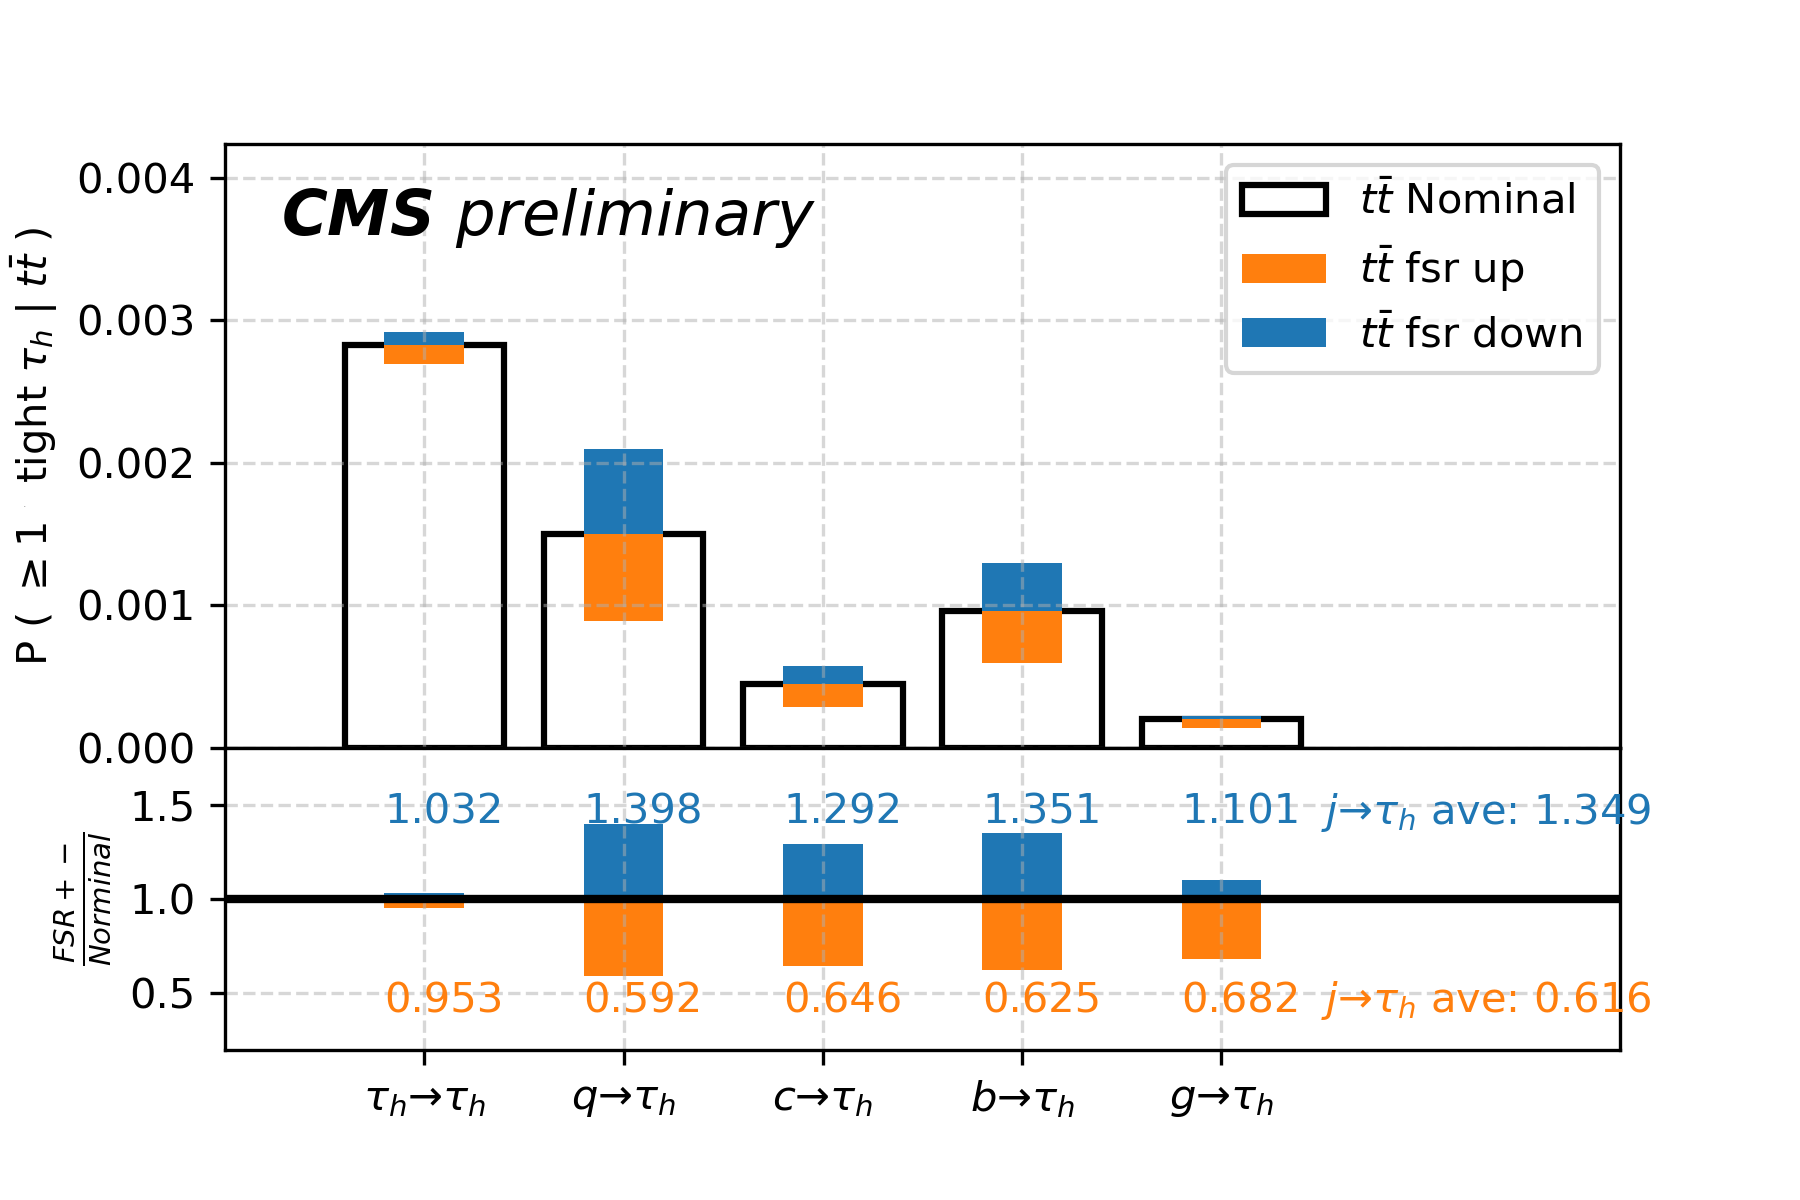
\includegraphics[width=0.49\textwidth]{chapters/Appendix/sectionTTSyst/figures/2020_MCRatio_fsr_tauGenFlavor_tauTight.png}
    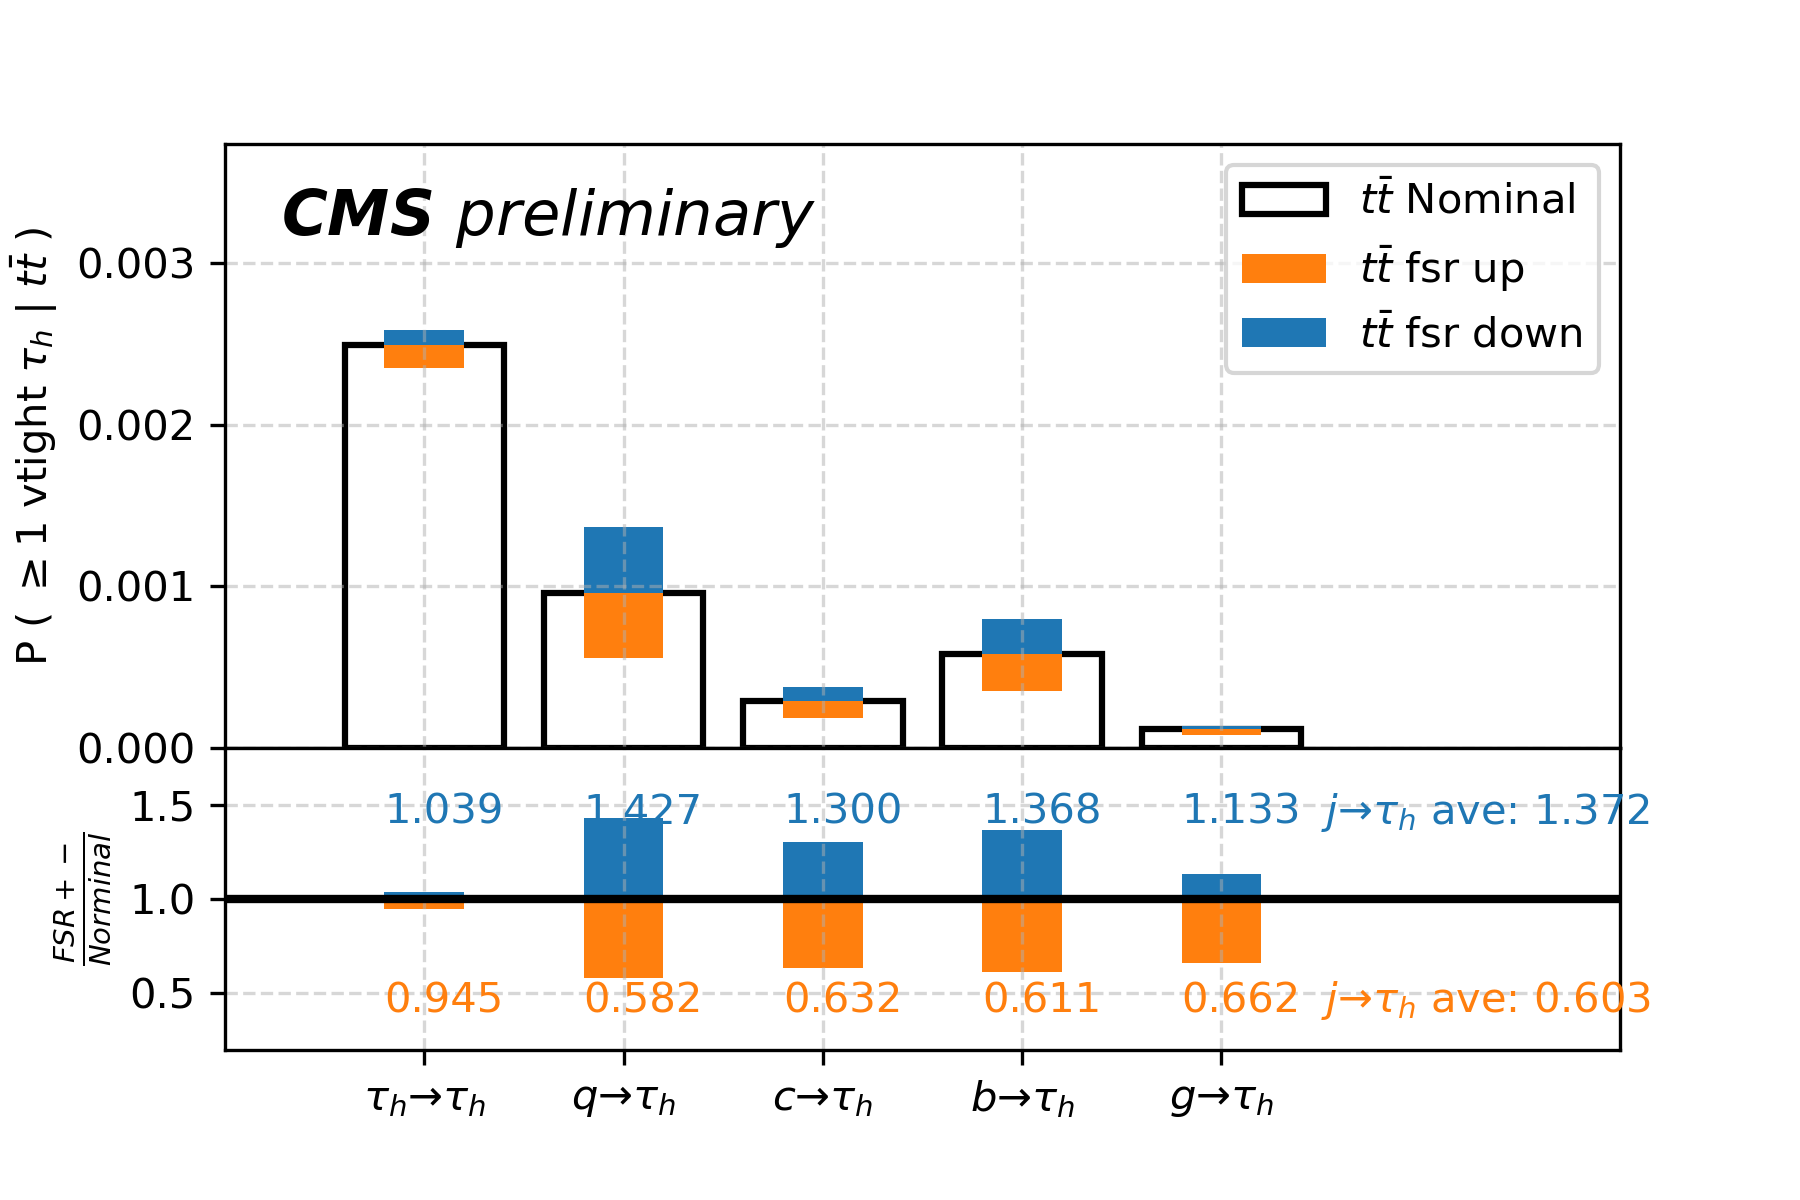
\includegraphics[width=0.49\textwidth]{chapters/Appendix/sectionTTSyst/figures/2020_MCRatio_fsr_tauGenFlavor_tauVTight.png}
    \caption{FSR effect on the $\tau_h$ identification and $j \to \tau_h$ misidentification obtained from the dedicated and the nominal \ttbar samples. 
    The Tight and VTight WP are shown on the left and right, respectively.
    }
    \label{fig:appendix:reweighttt:sf_fsr}
\end{figure}

\begin{figure}
    \centering
    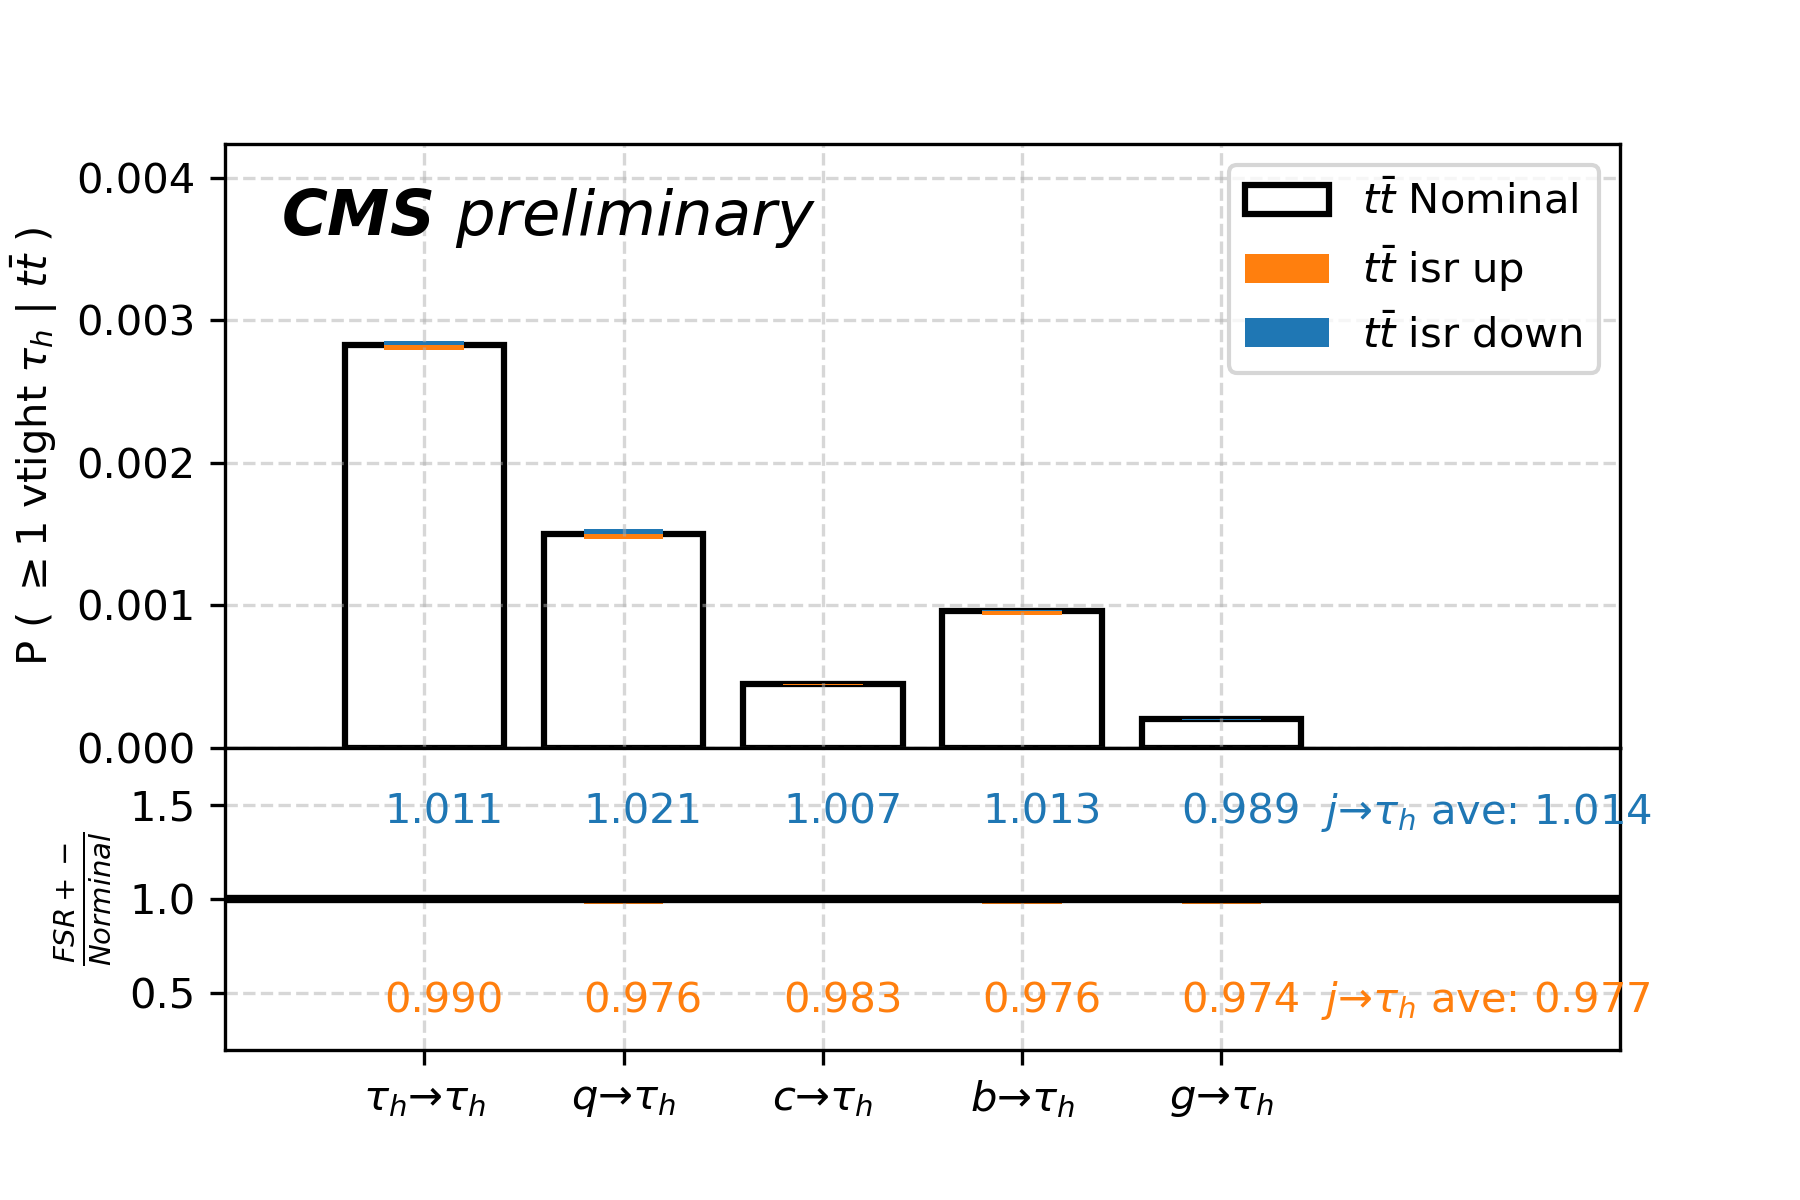
\includegraphics[width=0.49\textwidth]{chapters/Appendix/sectionTTSyst/figures/2020_MCRatio_isr_tauGenFlavor_tauTight.png}
    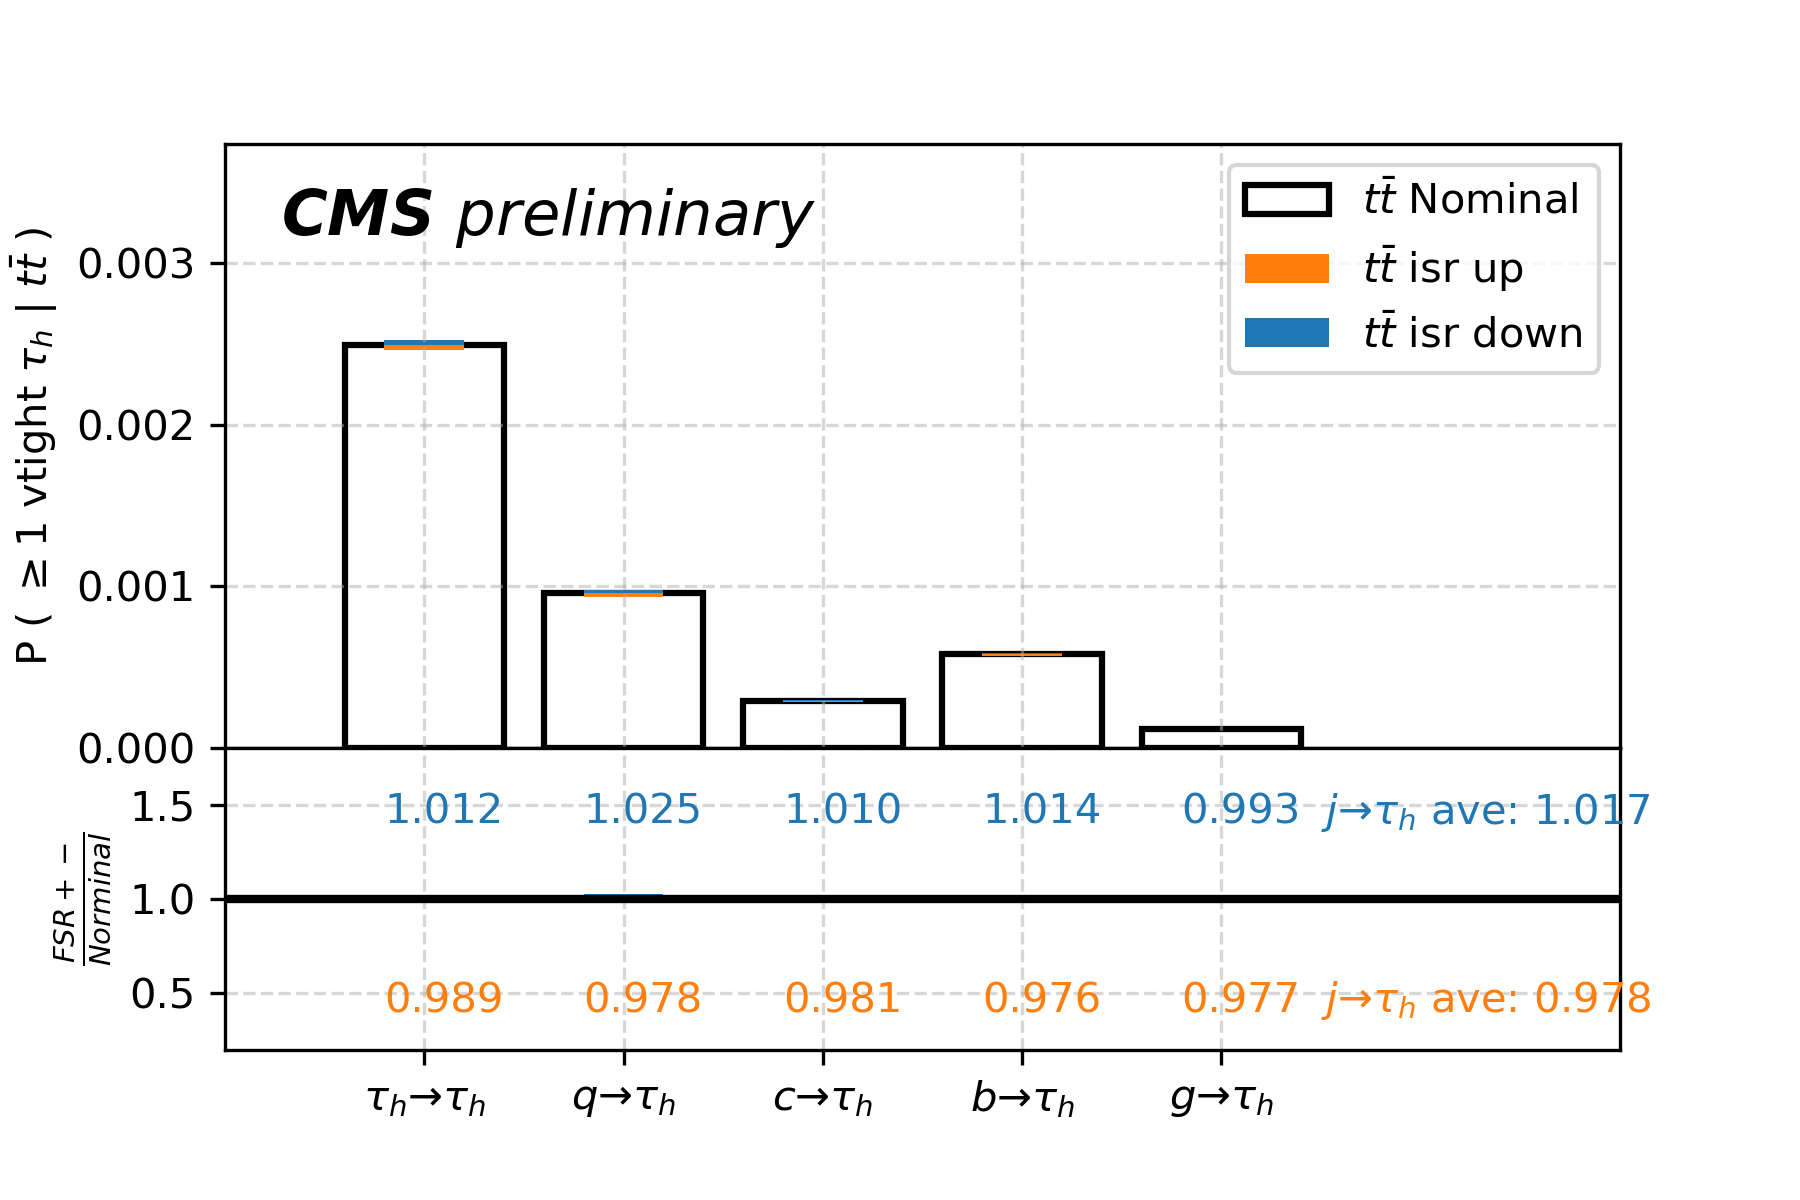
\includegraphics[width=0.49\textwidth]{chapters/Appendix/sectionTTSyst/figures/2020_MCRatio_isr_tauGenFlavor_tauVTight.png}
    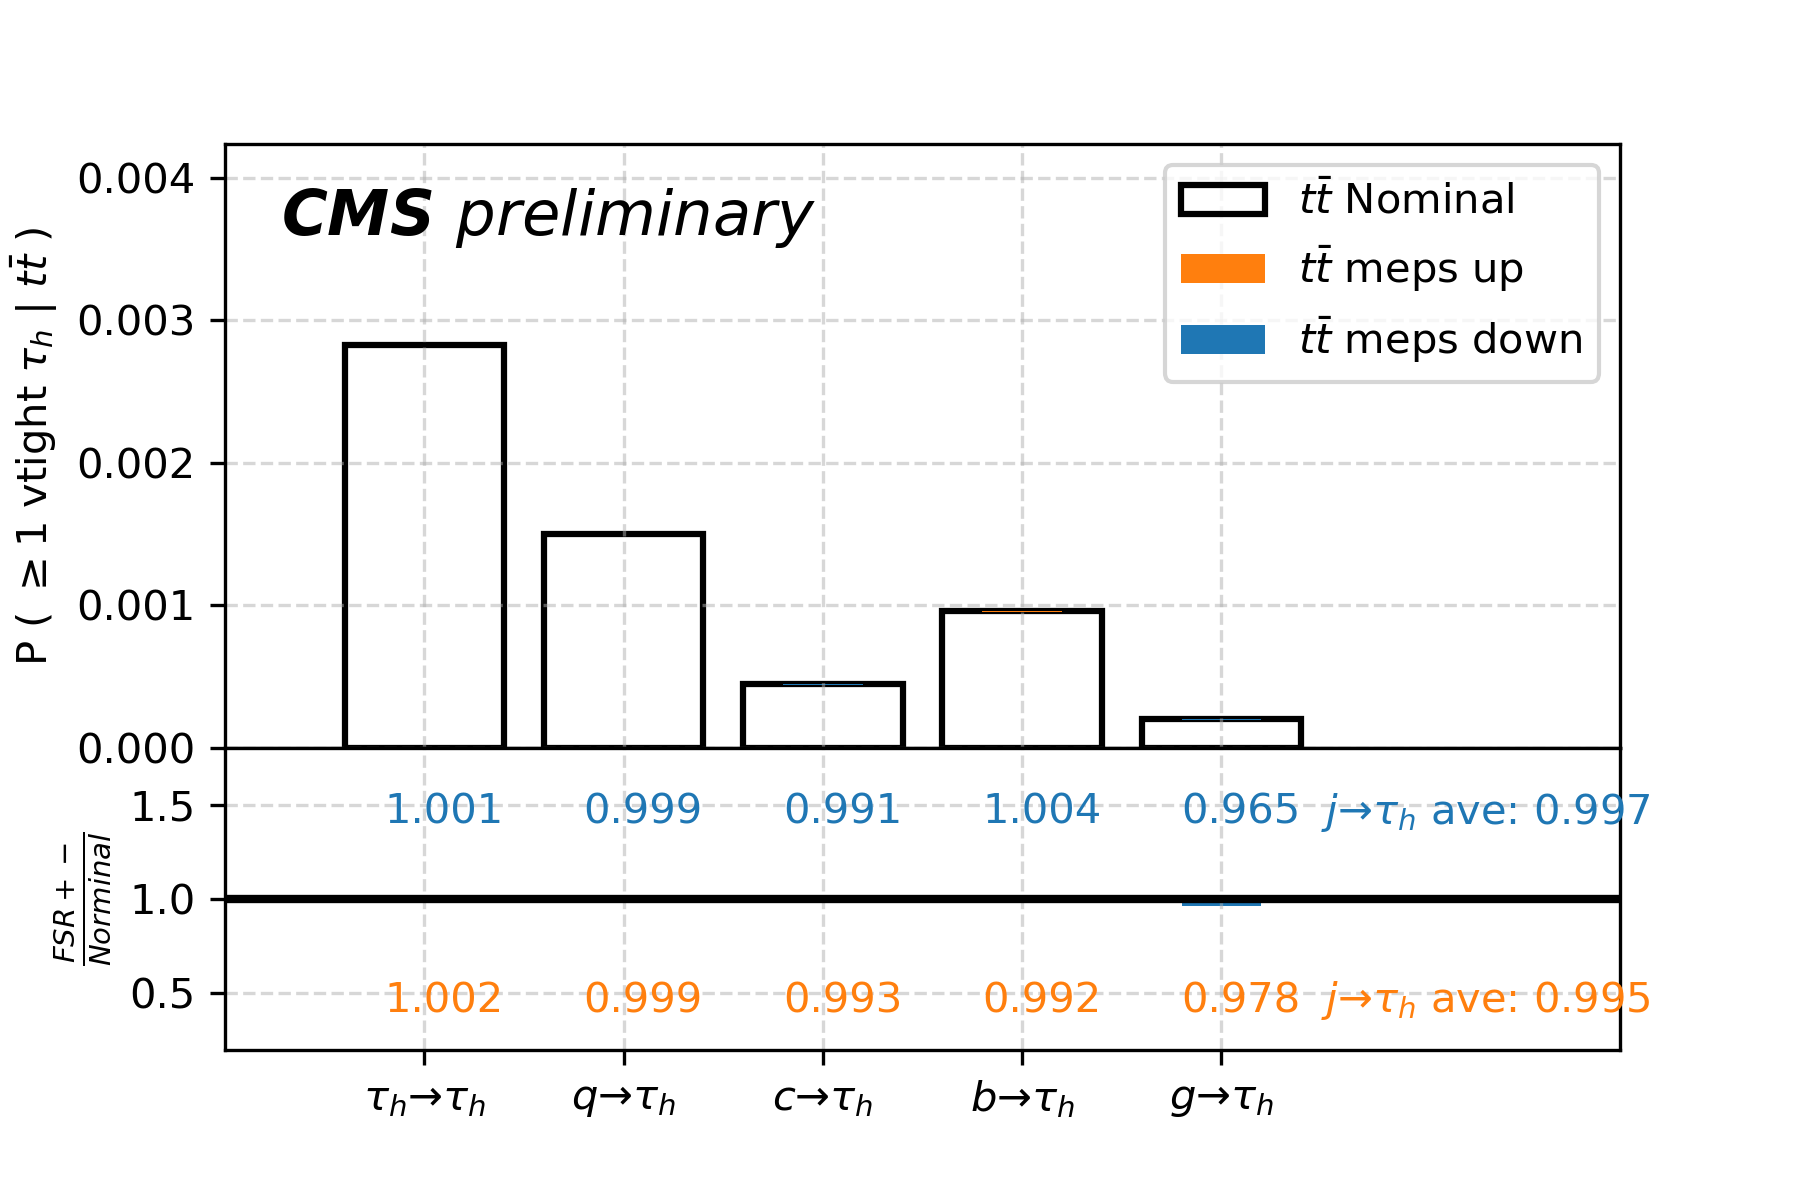
\includegraphics[width=0.49\textwidth]{chapters/Appendix/sectionTTSyst/figures/2020_MCRatio_meps_tauGenFlavor_tauTight.png}
    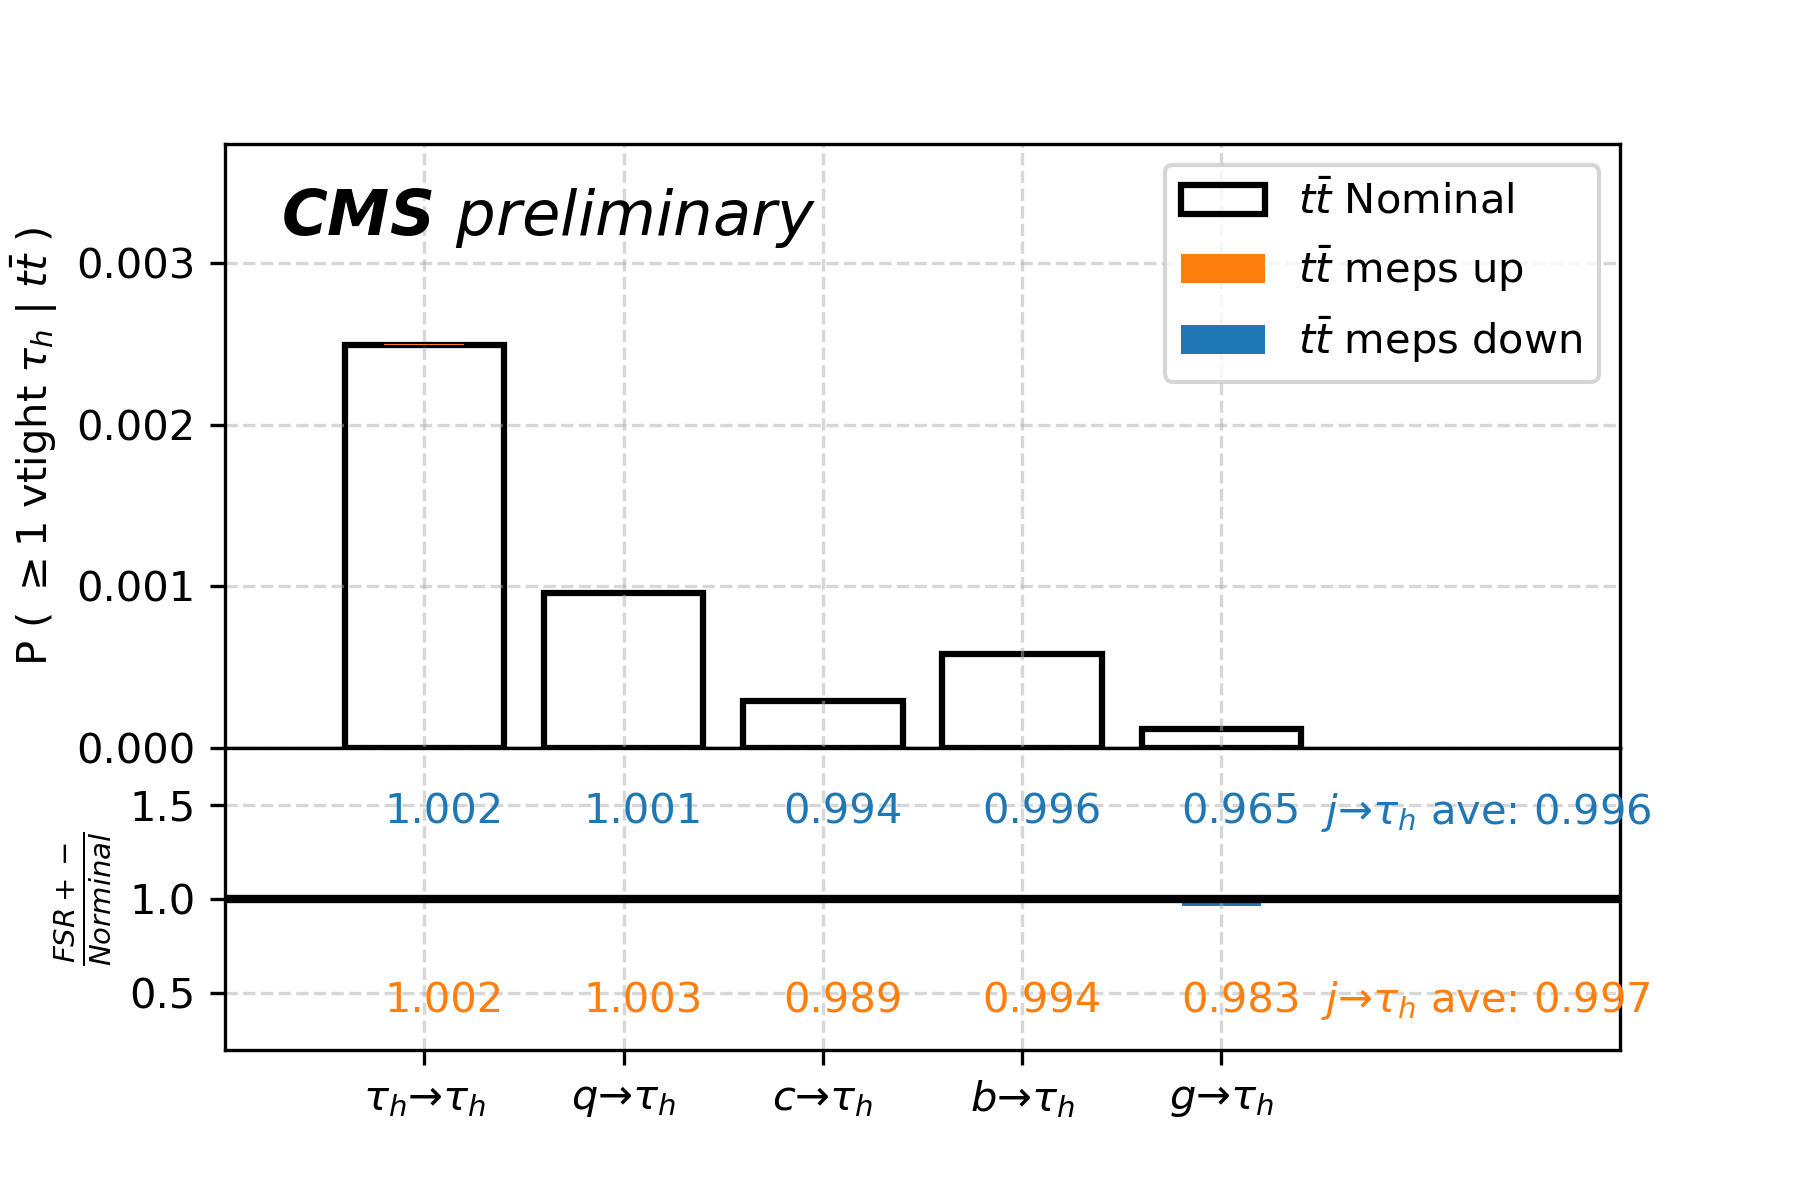
\includegraphics[width=0.49\textwidth]{chapters/Appendix/sectionTTSyst/figures/2020_MCRatio_meps_tauGenFlavor_tauVTight.png}
    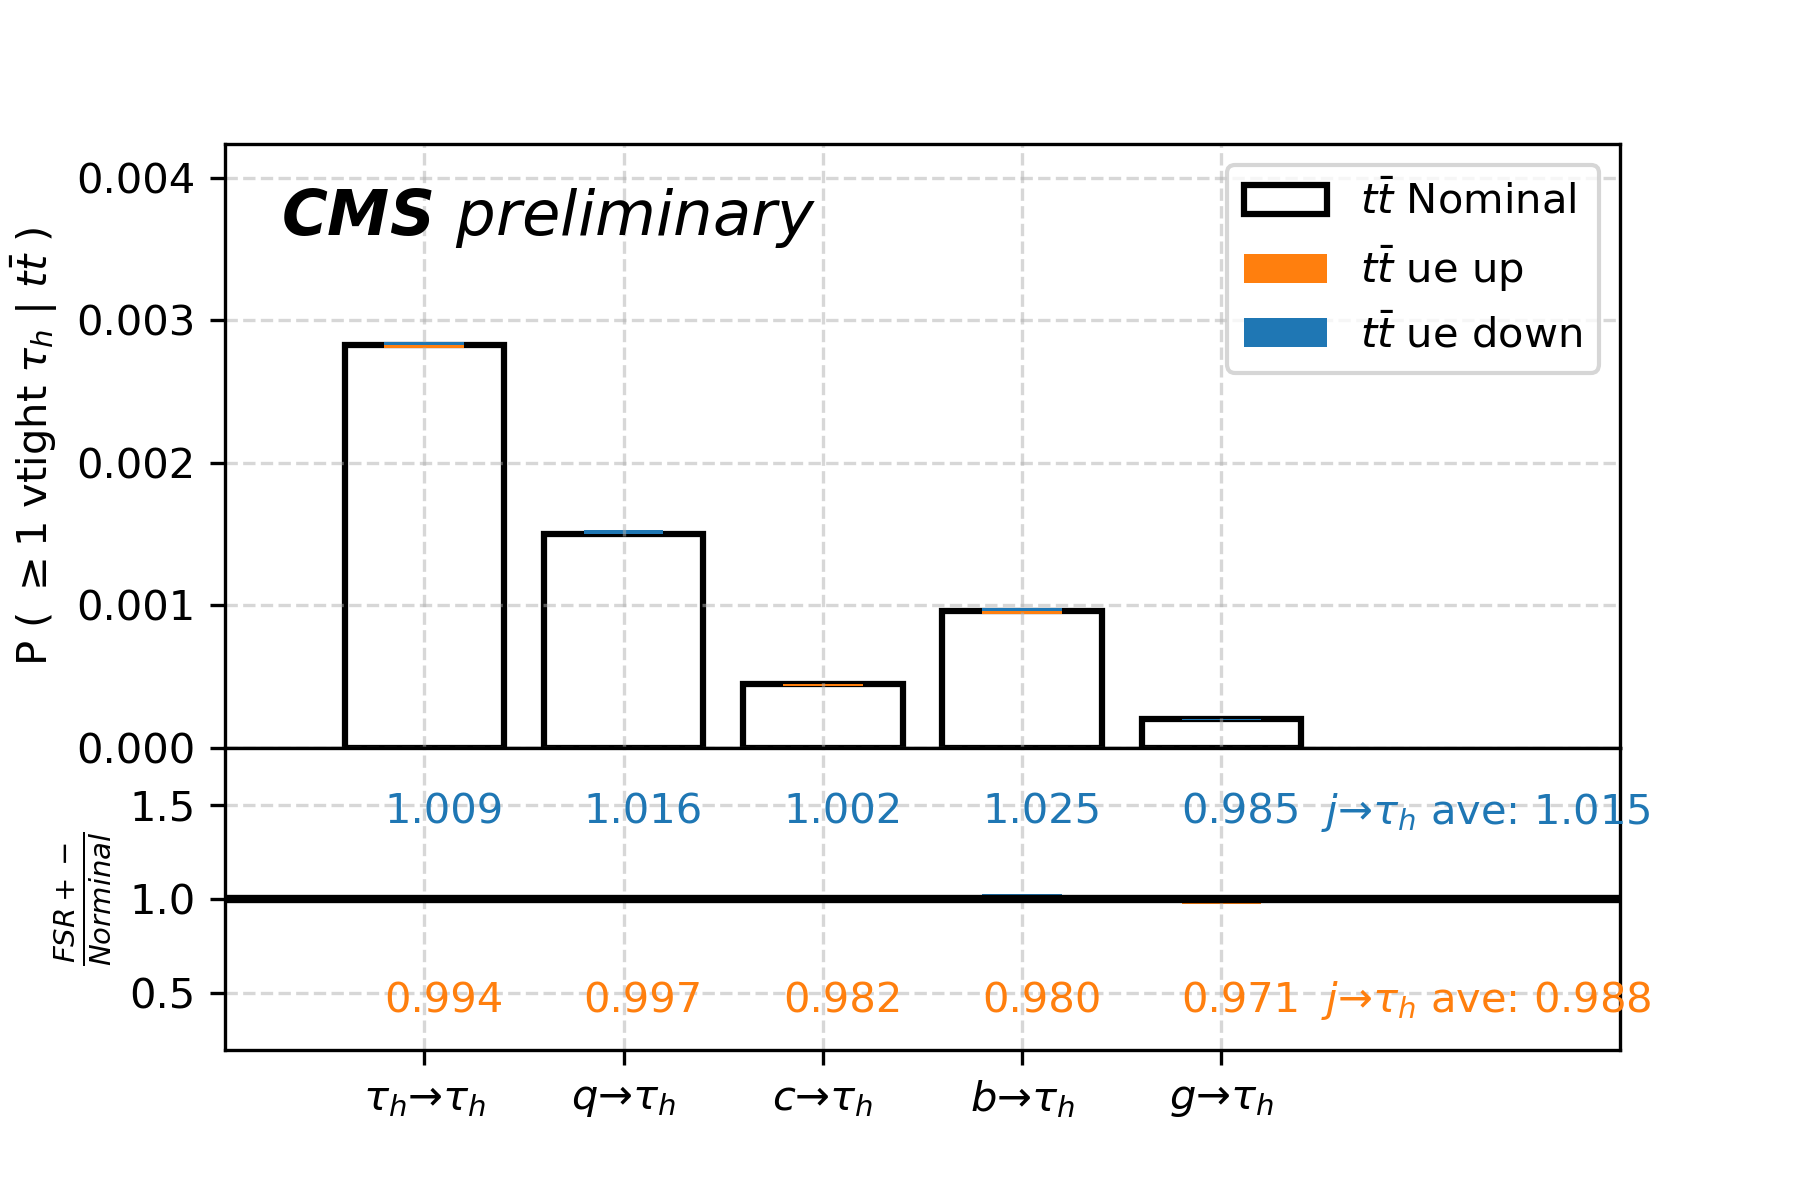
\includegraphics[width=0.49\textwidth]{chapters/Appendix/sectionTTSyst/figures/2020_MCRatio_ue_tauGenFlavor_tauTight.png}
    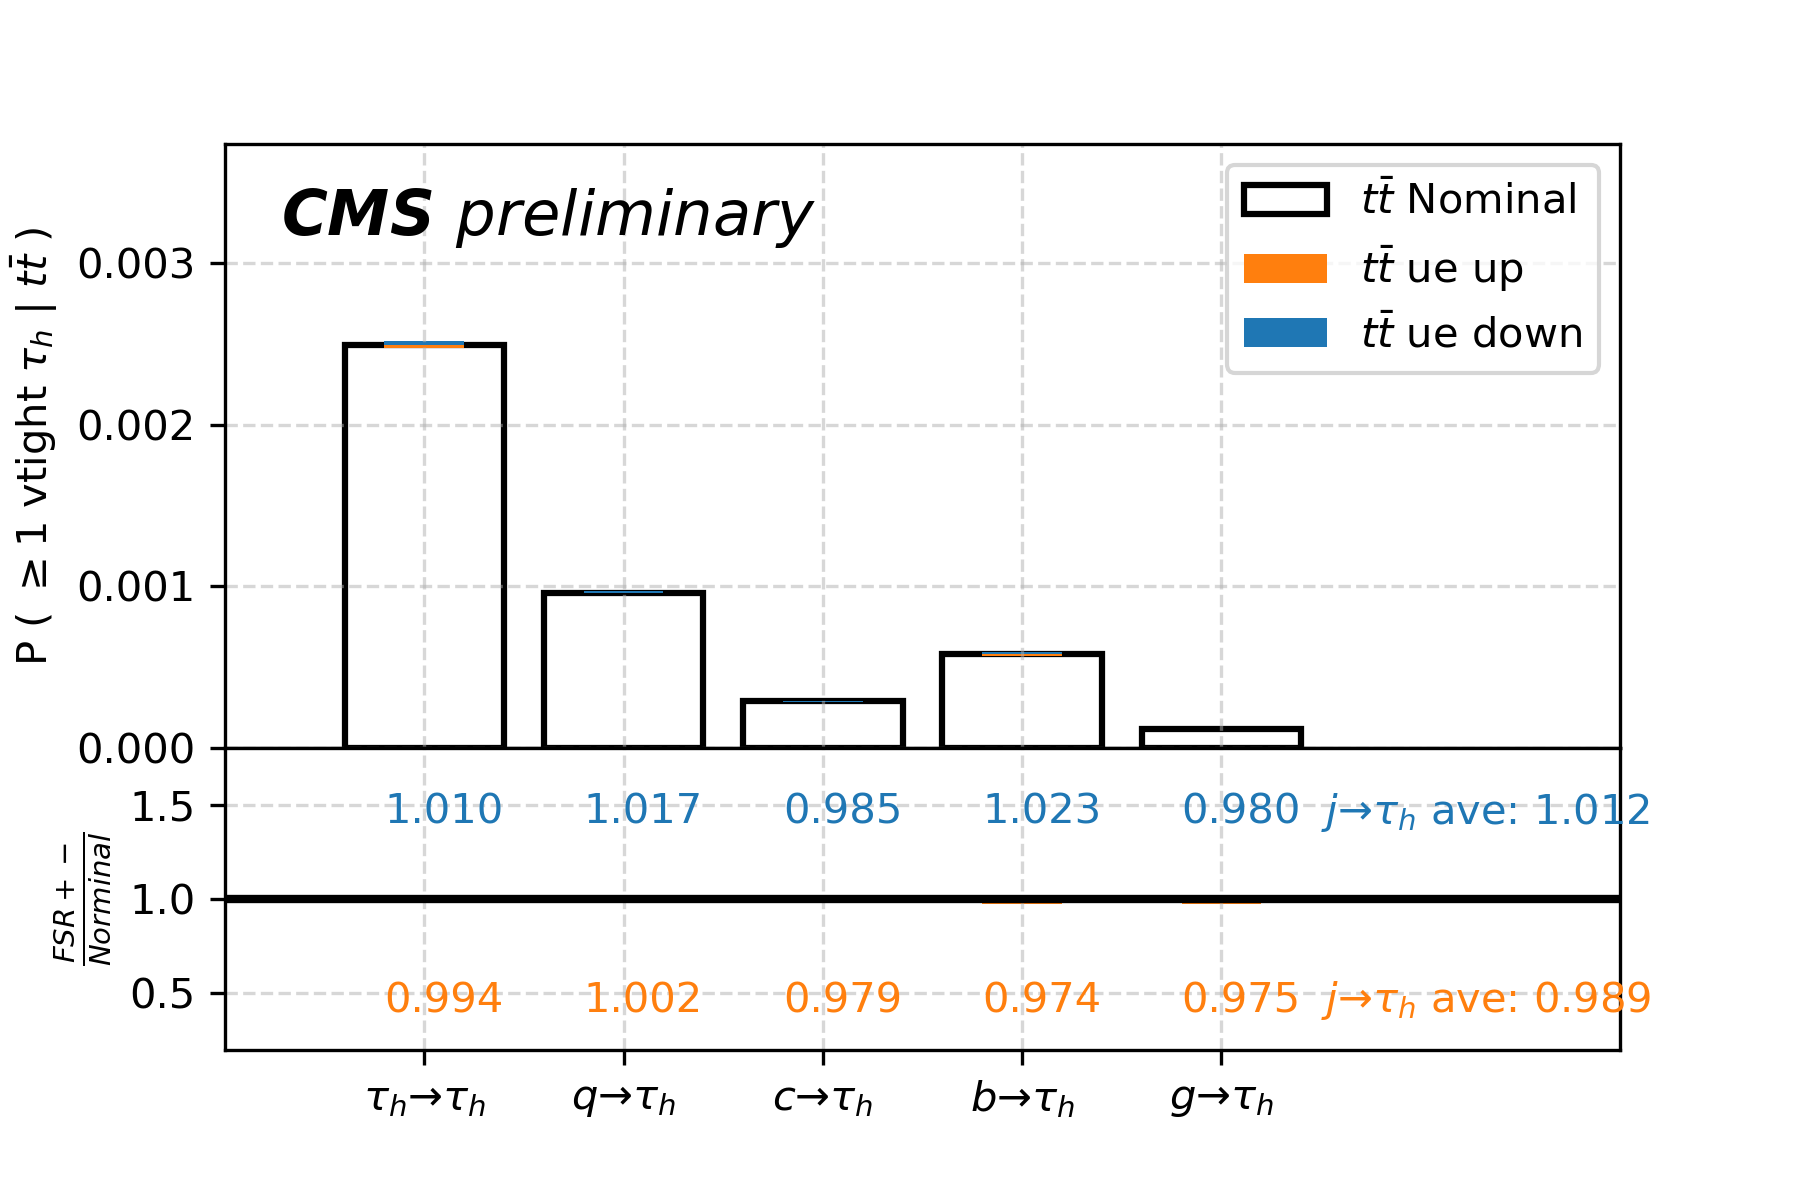
\includegraphics[width=0.49\textwidth]{chapters/Appendix/sectionTTSyst/figures/2020_MCRatio_ue_tauGenFlavor_tauVTight.png}
    \caption{ISR, MEPS, UE effect on the $\tau_h$ identification and $j \to \tau_h$ misidentification obtained from the dedicated and the nominal \ttbar samples.
    The Tight and VTight WP are shown on the left and right, respectively.
    }
    \label{fig:appendix:reweighttt:sf_isr_MEPS_UE}
\end{figure}




\begin{table}[h]
    \centering
    \caption{Comparison between nominal uncertainty (in a snapshot of
        the analysis) and the uncertainty after applying the corrections
        to the FSR variation.}
        
    \begin{tabular}{l|cccc}
                                  & $W\rightarrow e$ & $W\rightarrow \mu$ & $W\rightarrow \tau$ & $W\rightarrow h$ \\
        \hline
        nominal                   & 1.02             & 0.71               & 2.04                & 0.40             \\
        w/ $\tau$ FSR corrections & 1.01             & 0.69               & 1.69                & 0.36             \\
    \end{tabular}
    \label{fig:fsr_correction}
\end{table}


Table~\label{fig:fsr_correction} shows total uncertainties of $Br(W)$ due 
to FSR before and after the tau id and misid correction of the dedicated FSR sample.
Before the correction, the dedicated FSR sample leads to an artificially large
uncertainties which double counts the tau id and misid systematics.




The FSR dedicated \ttbar samples are corrected using the SF in Figure~\ref{fig:appendix:reweighttt:sf_fsr}.
The up and down variation given by the dedicated MC samples lead to envelops on the \ttbar event efficiencies.
As discussed in section~\ref{sec:analysis:method}, there are 21 \ttbar event efficiencies with 21 different
$WW$ decay scenarios. For VTight WP, the 21 envelops on efficiencies due to FSR, ISR, MEPS, and UE are shown in 
Figure~\ref{fig:appendix:reweighttt:effAfterCorrFSR}-\ref{fig:appendix:reweighttt:effAfterCorrUE}. 
Due to the finite statistics of the dedicated MC samples, the envelops edges are smear by the MC statistics, 
which are also shown in the Figure~\ref{fig:appendix:reweighttt:effAfterCorrFSR}-\ref{fig:appendix:reweighttt:effAfterCorrUE}.


\begin{figure}
    \centering
    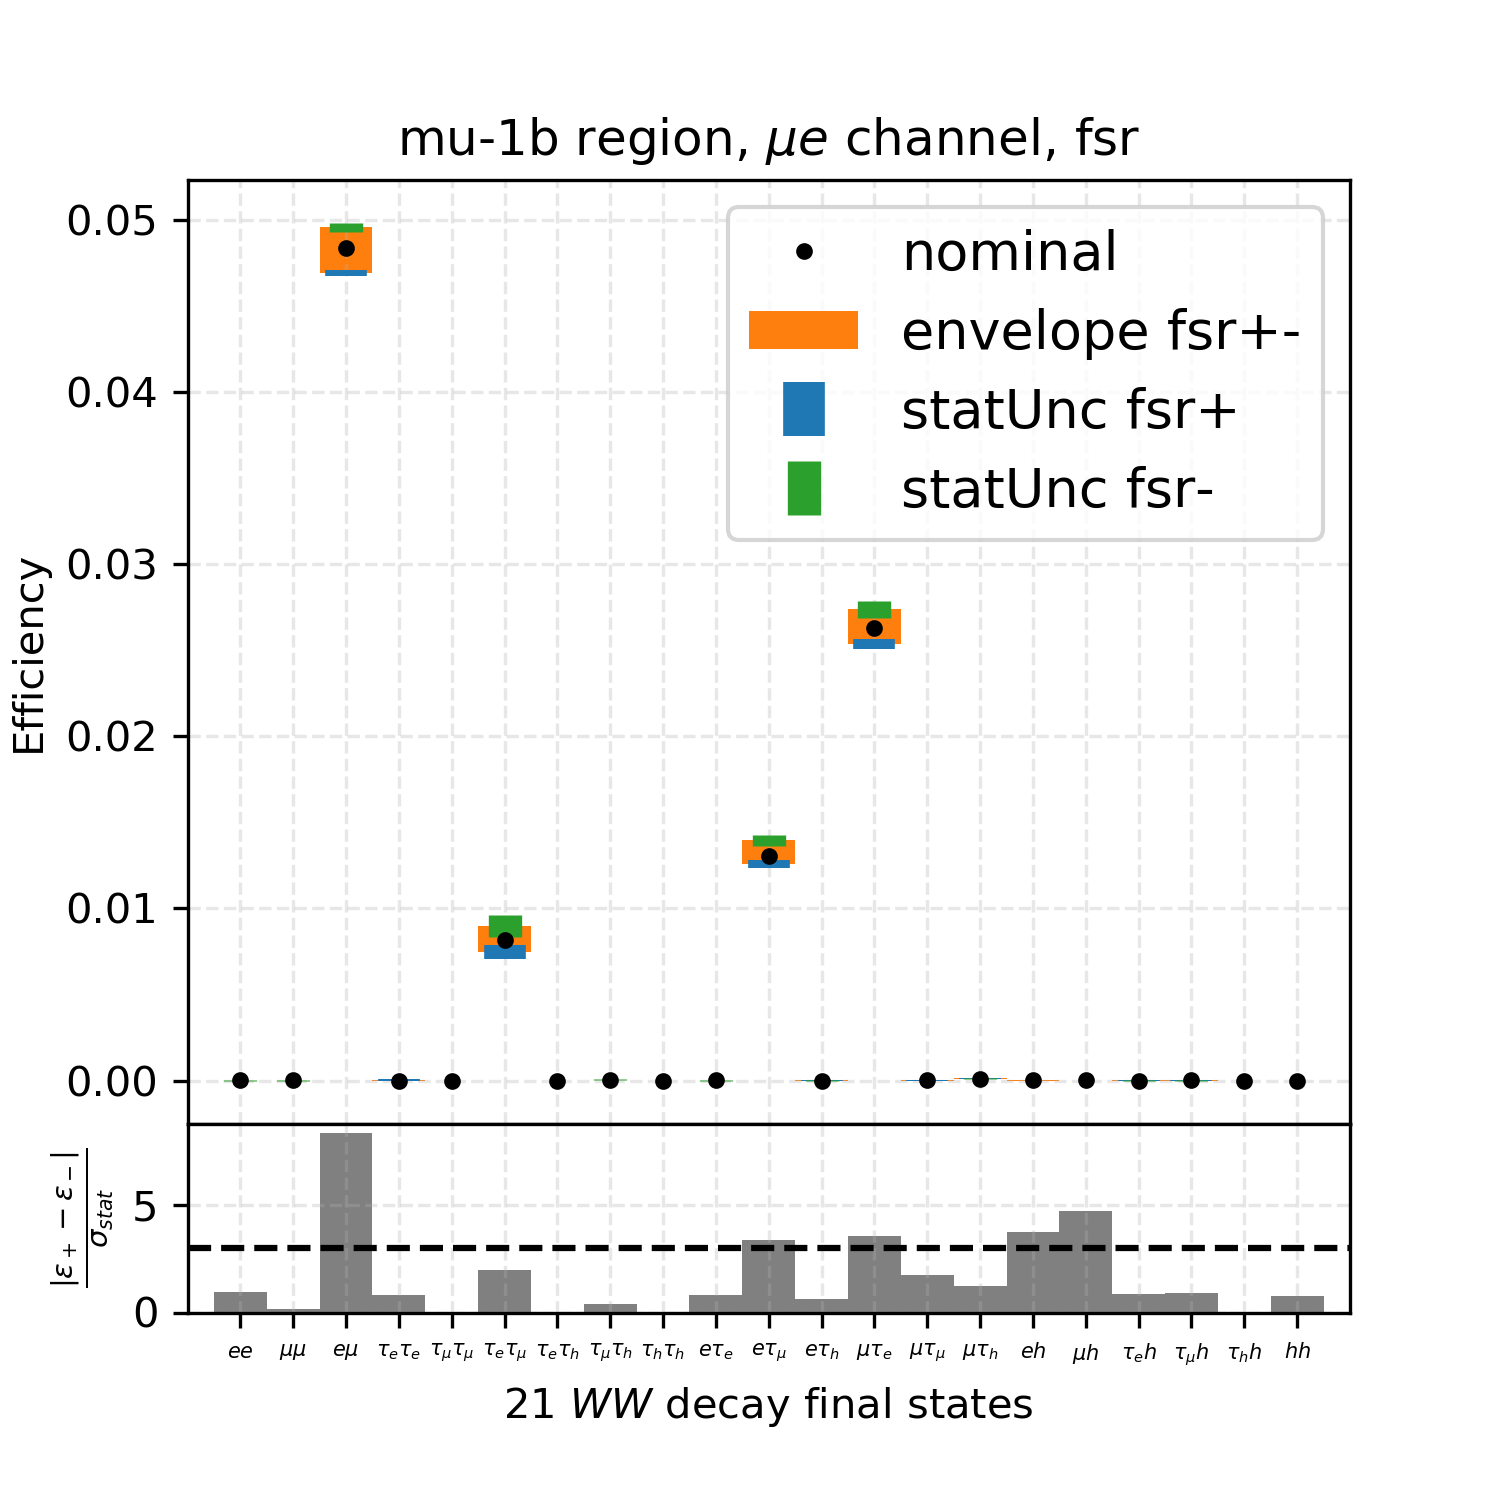
\includegraphics[width=0.24\textwidth]{chapters/Appendix/sectionTTSyst/figures/afterCorr/icata0_ch0_fsr.png}
    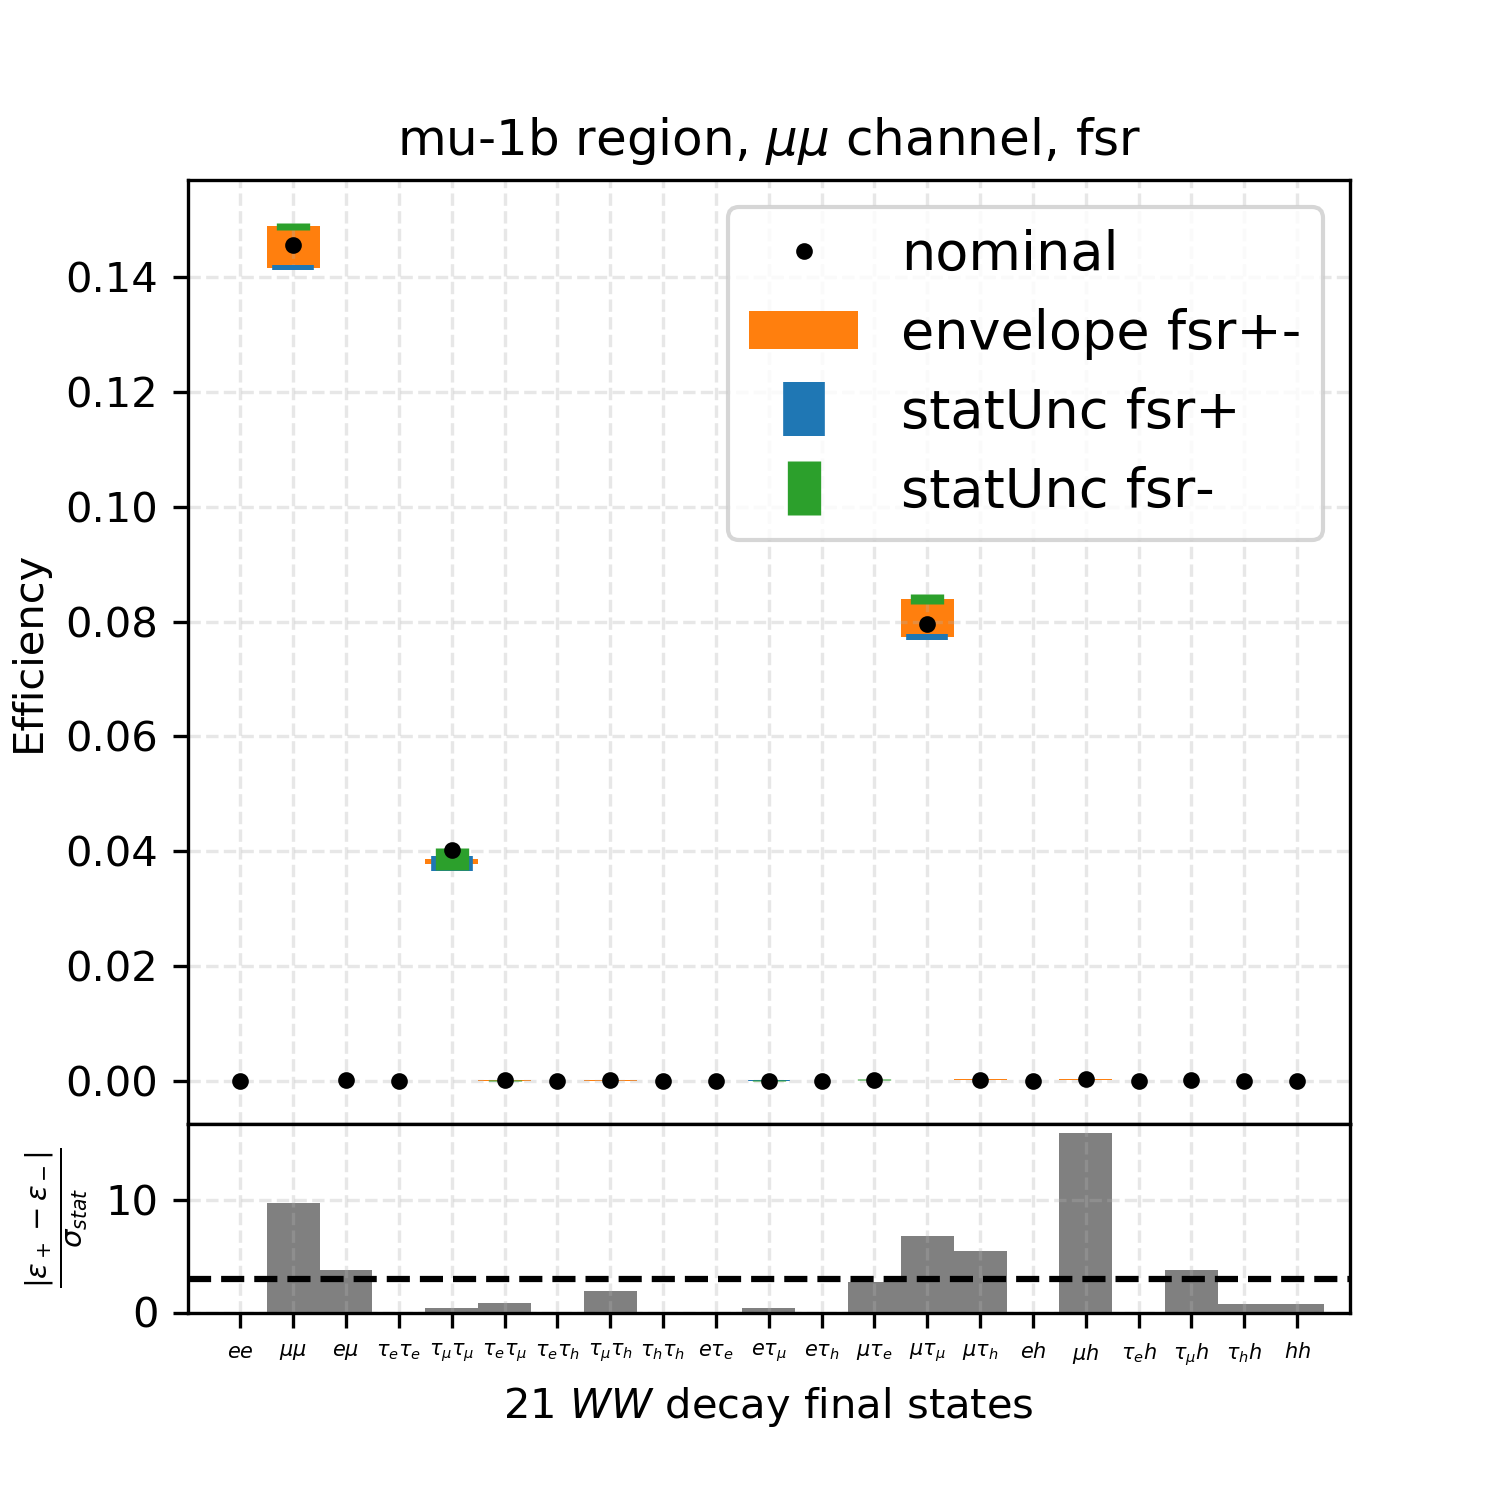
\includegraphics[width=0.24\textwidth]{chapters/Appendix/sectionTTSyst/figures/afterCorr/icata0_ch1_fsr.png}
    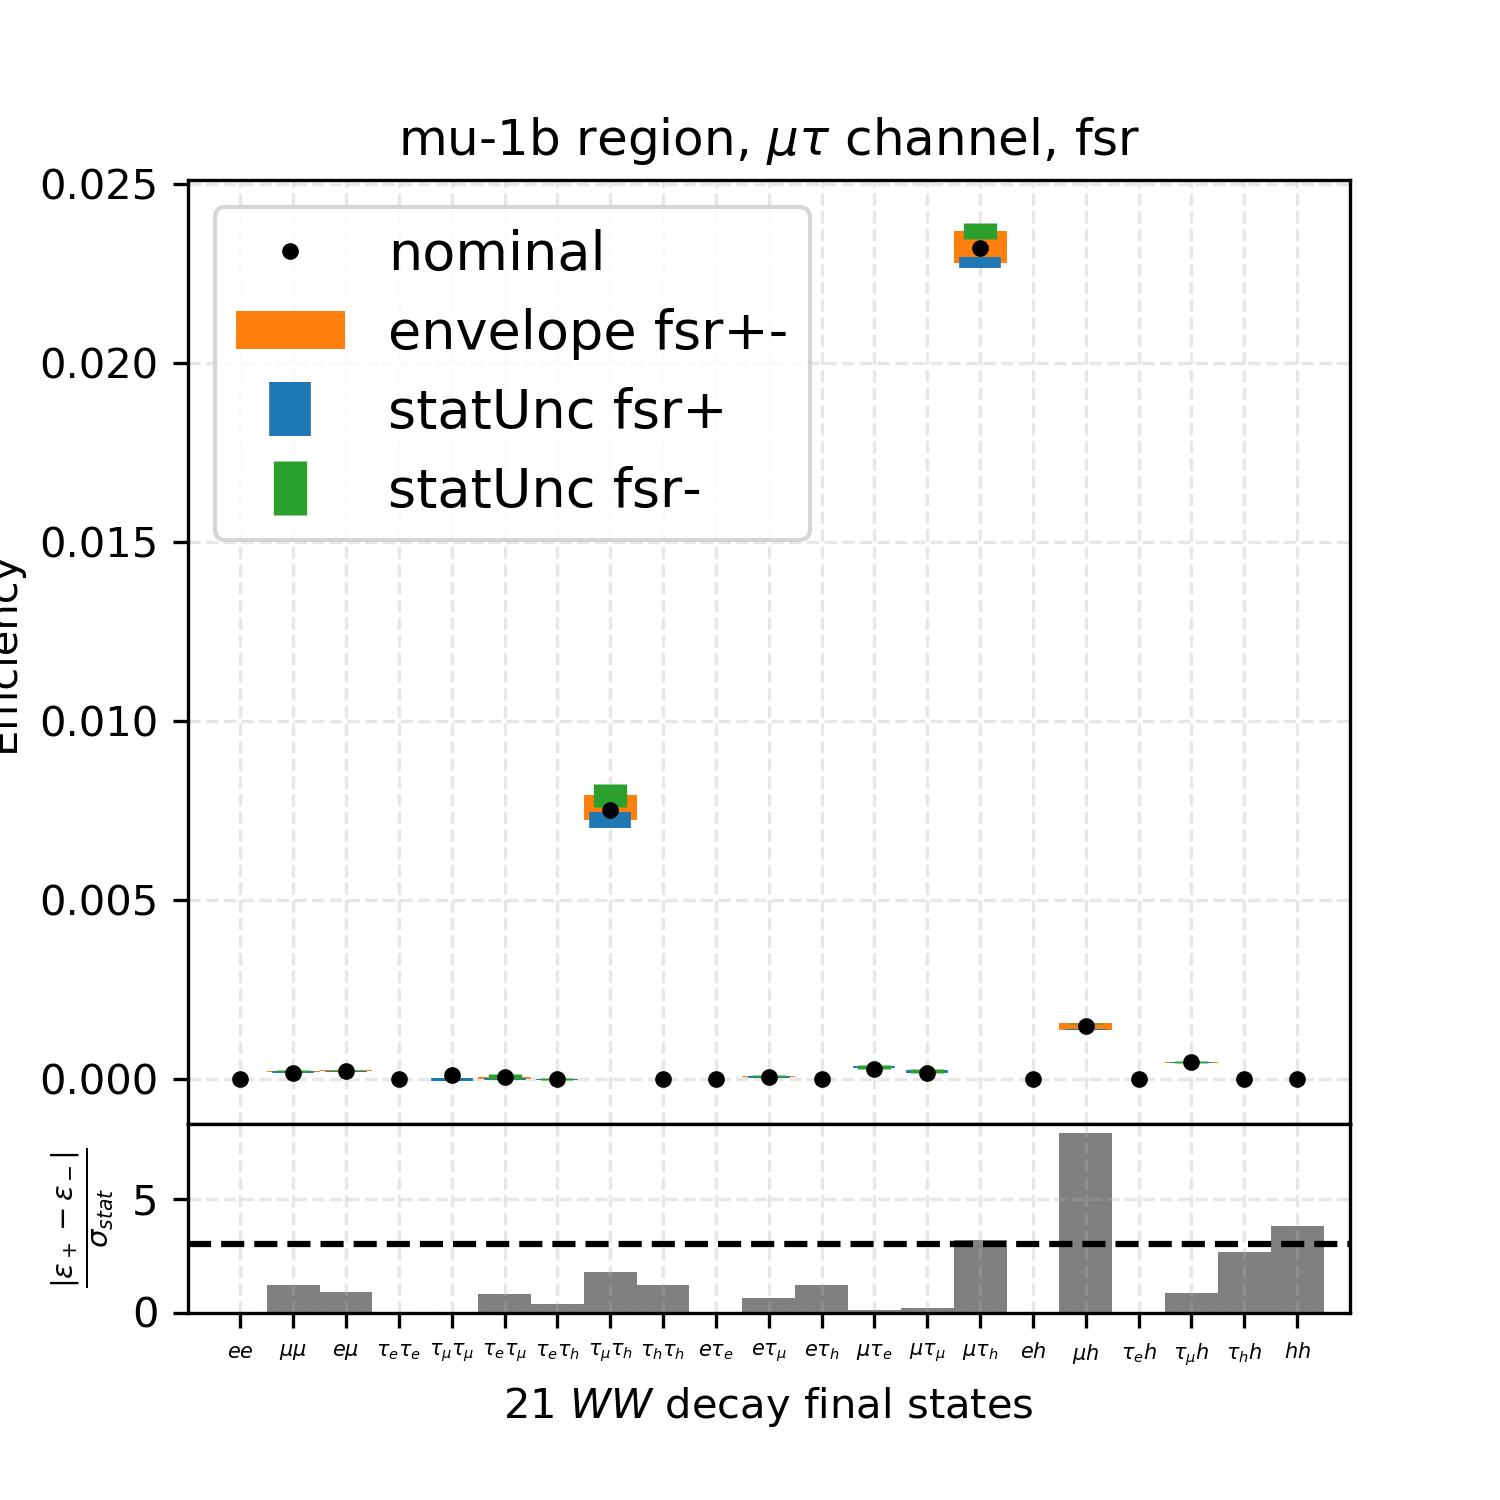
\includegraphics[width=0.24\textwidth]{chapters/Appendix/sectionTTSyst/figures/afterCorr/icata0_ch2_fsr.png}
    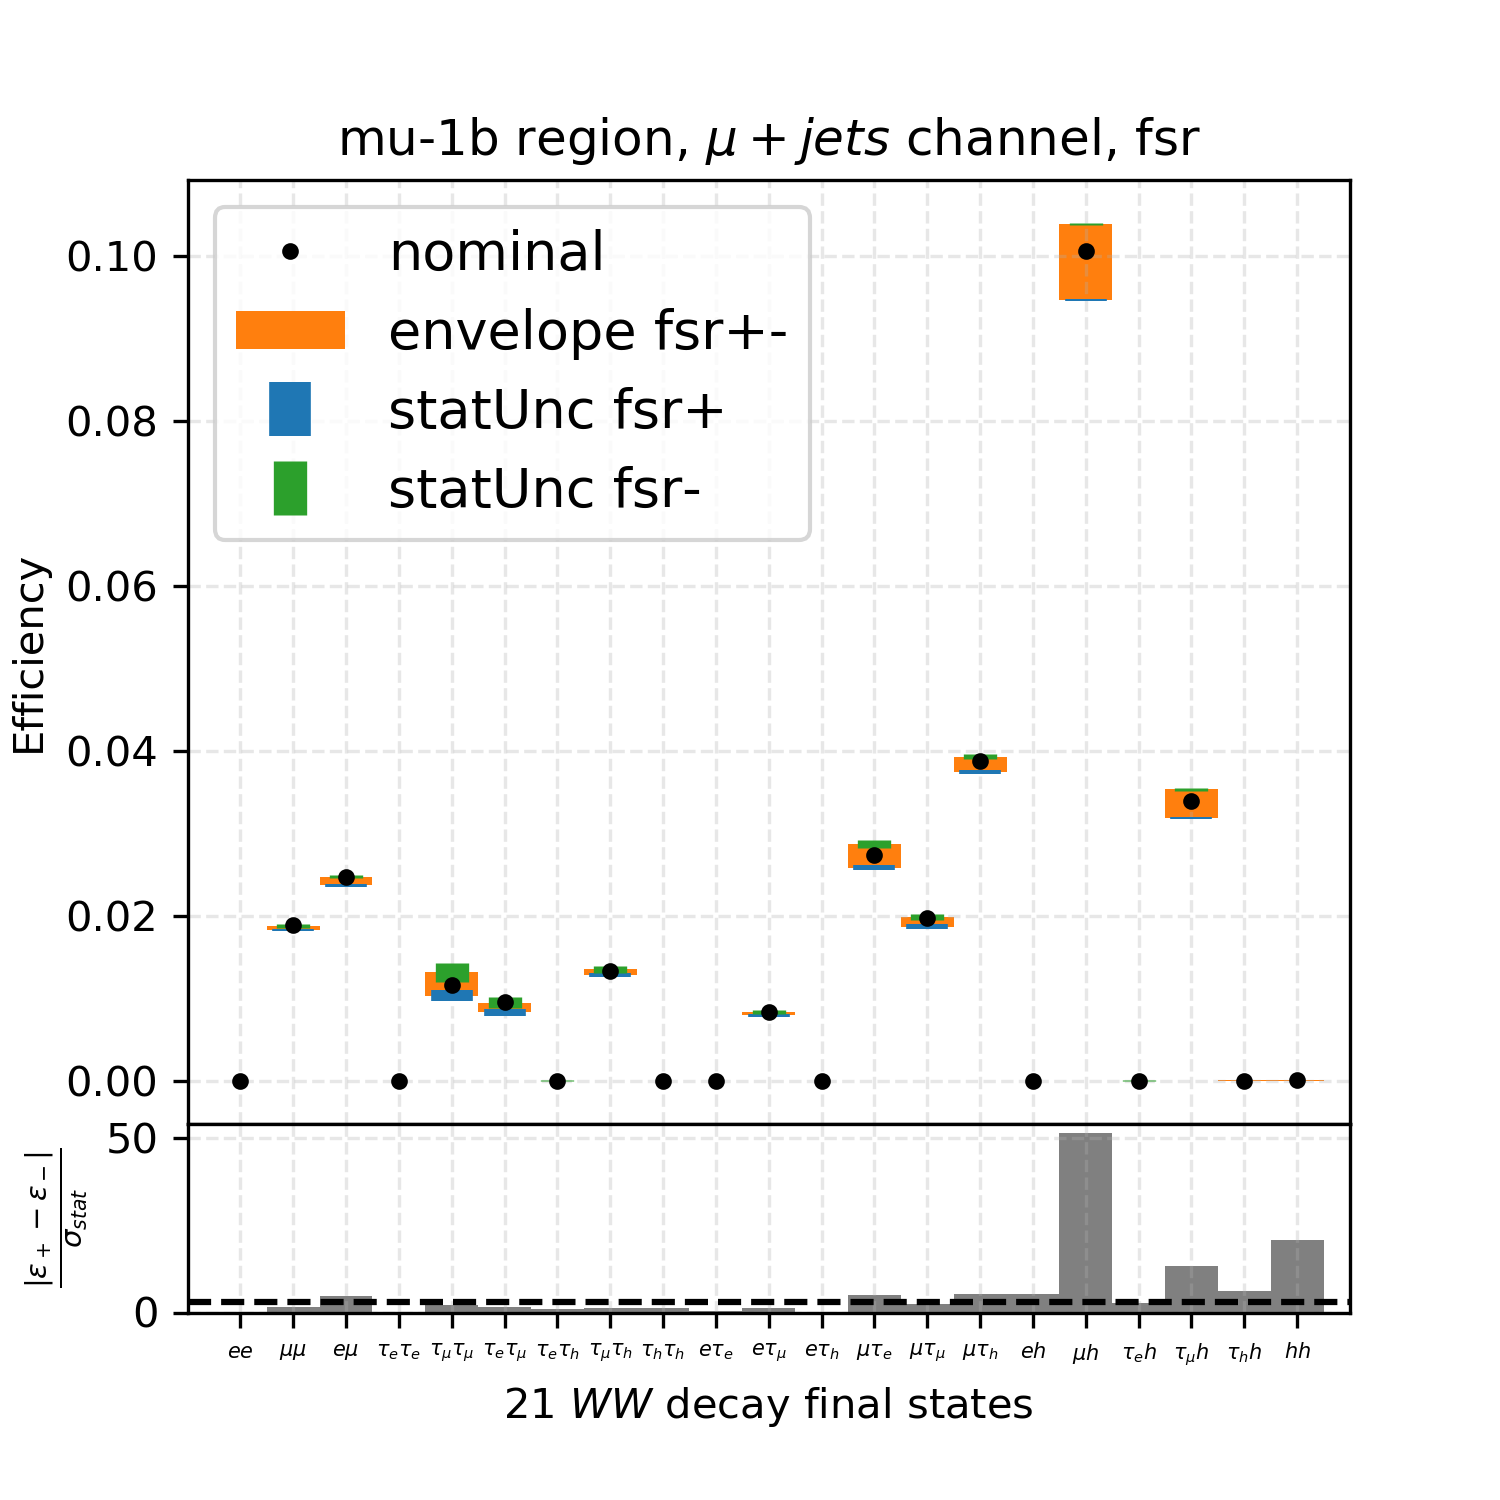
\includegraphics[width=0.24\textwidth]{chapters/Appendix/sectionTTSyst/figures/afterCorr/icata0_ch3_fsr.png}

    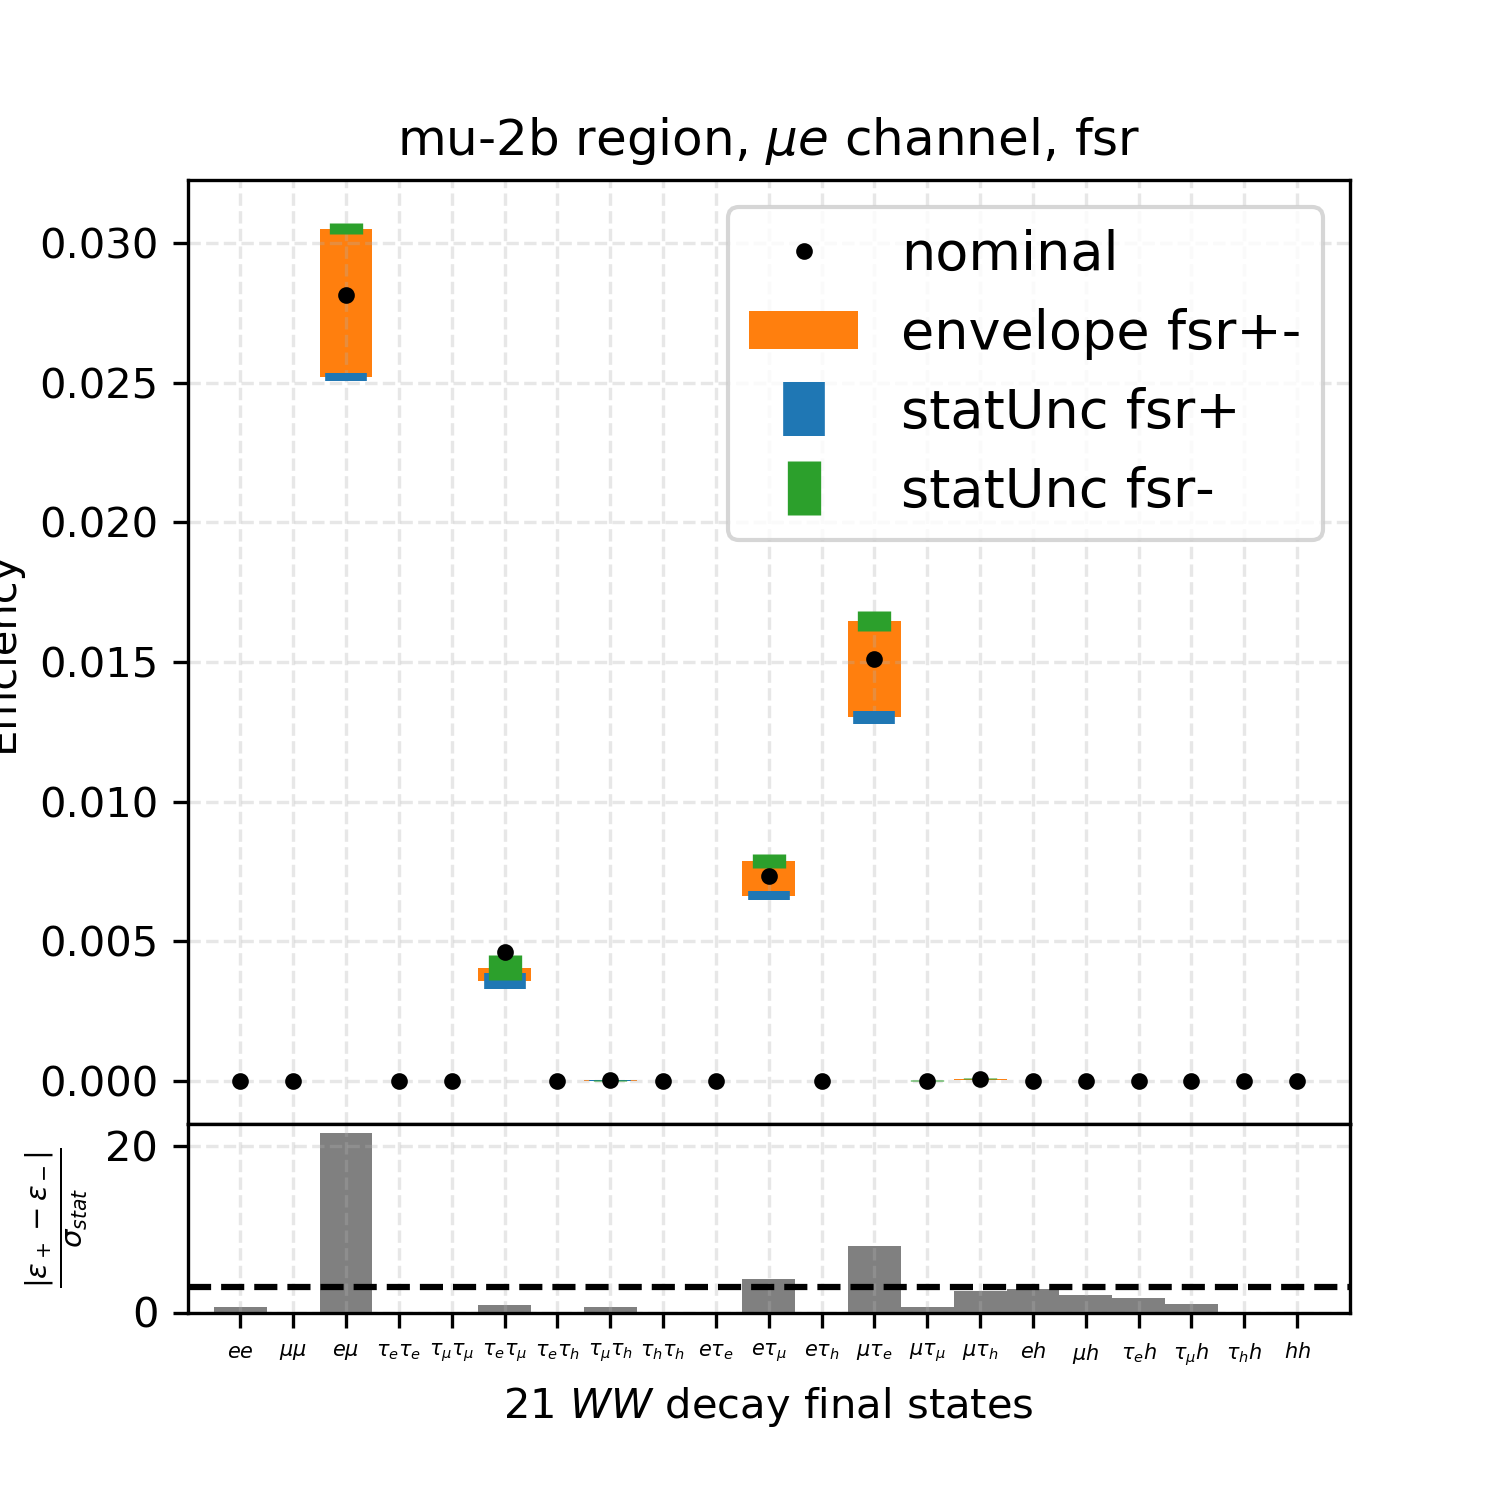
\includegraphics[width=0.24\textwidth]{chapters/Appendix/sectionTTSyst/figures/afterCorr/icata1_ch0_fsr.png}
    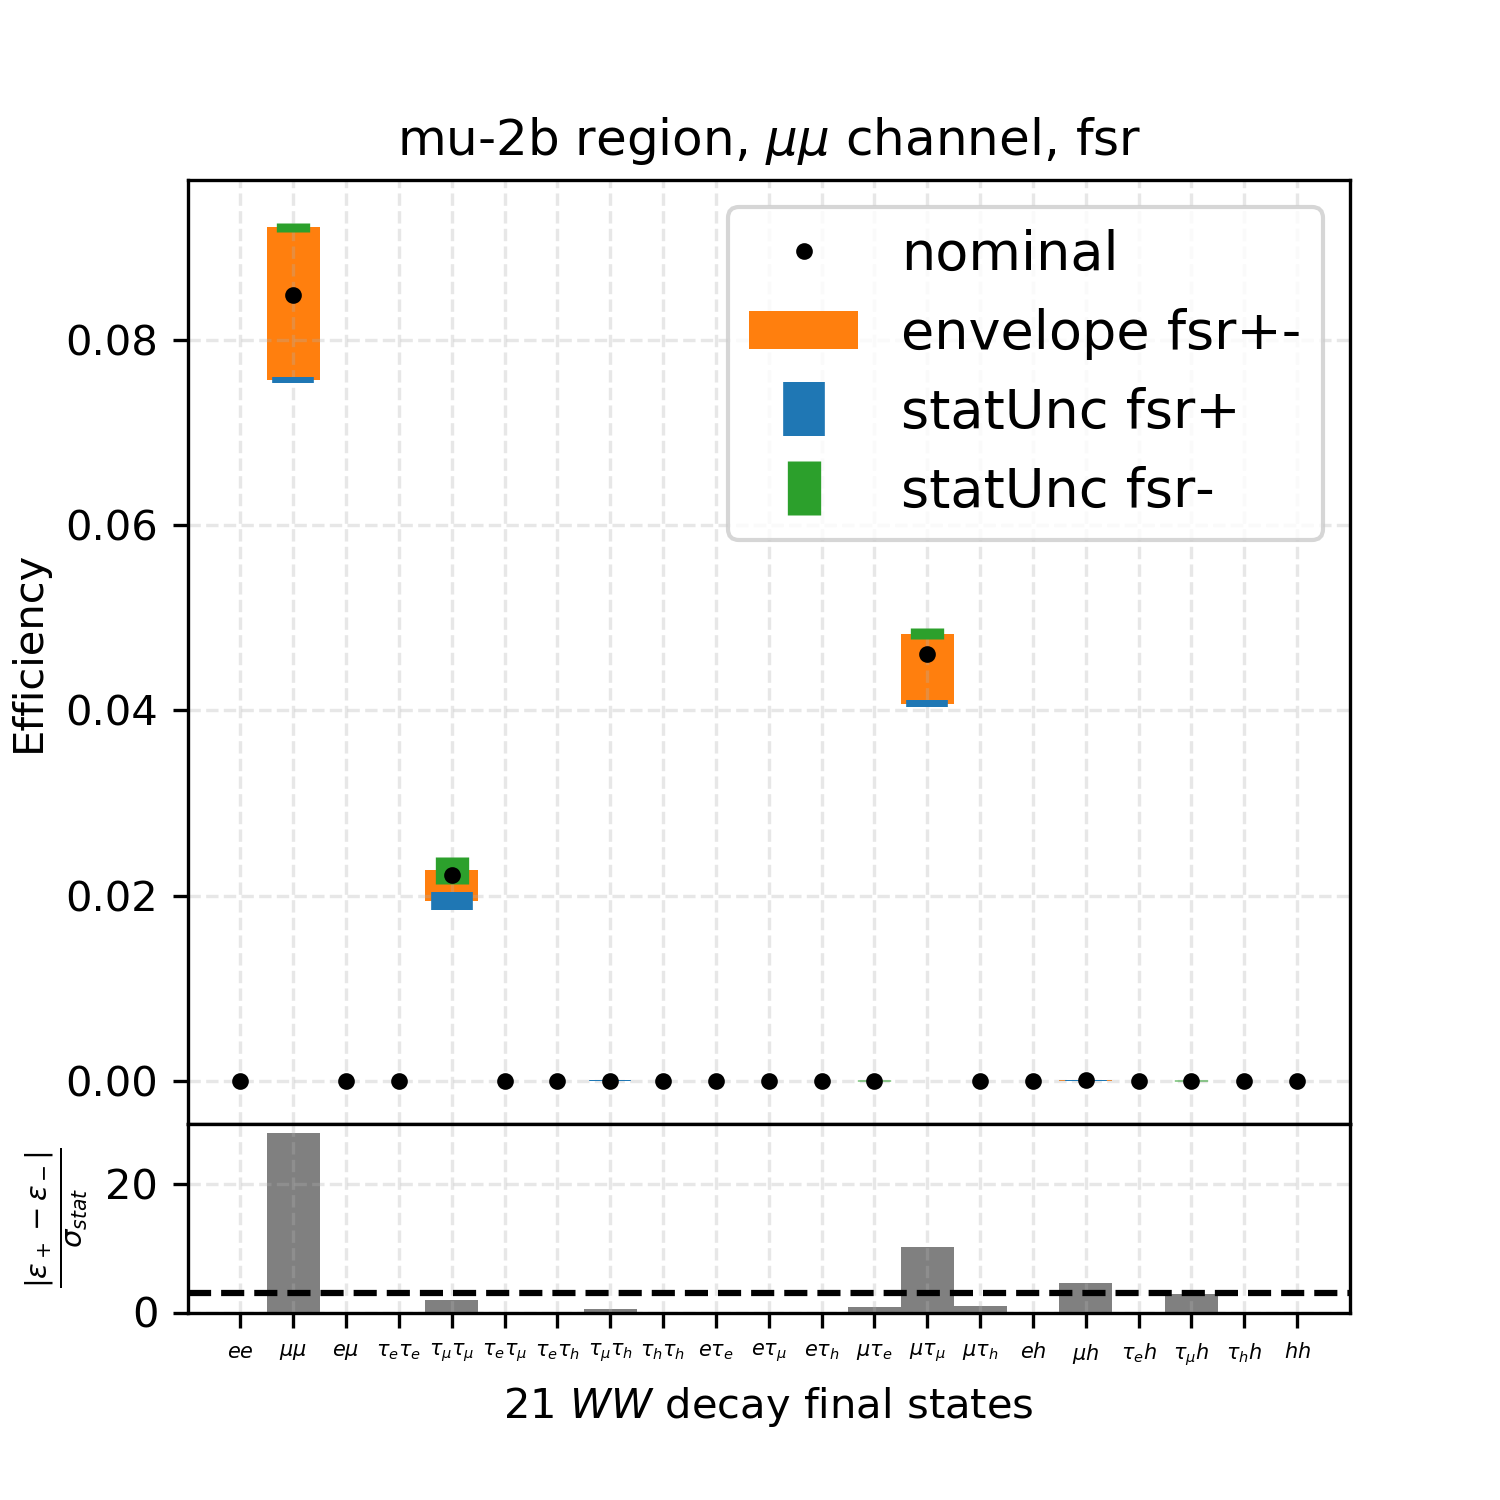
\includegraphics[width=0.24\textwidth]{chapters/Appendix/sectionTTSyst/figures/afterCorr/icata1_ch1_fsr.png}
    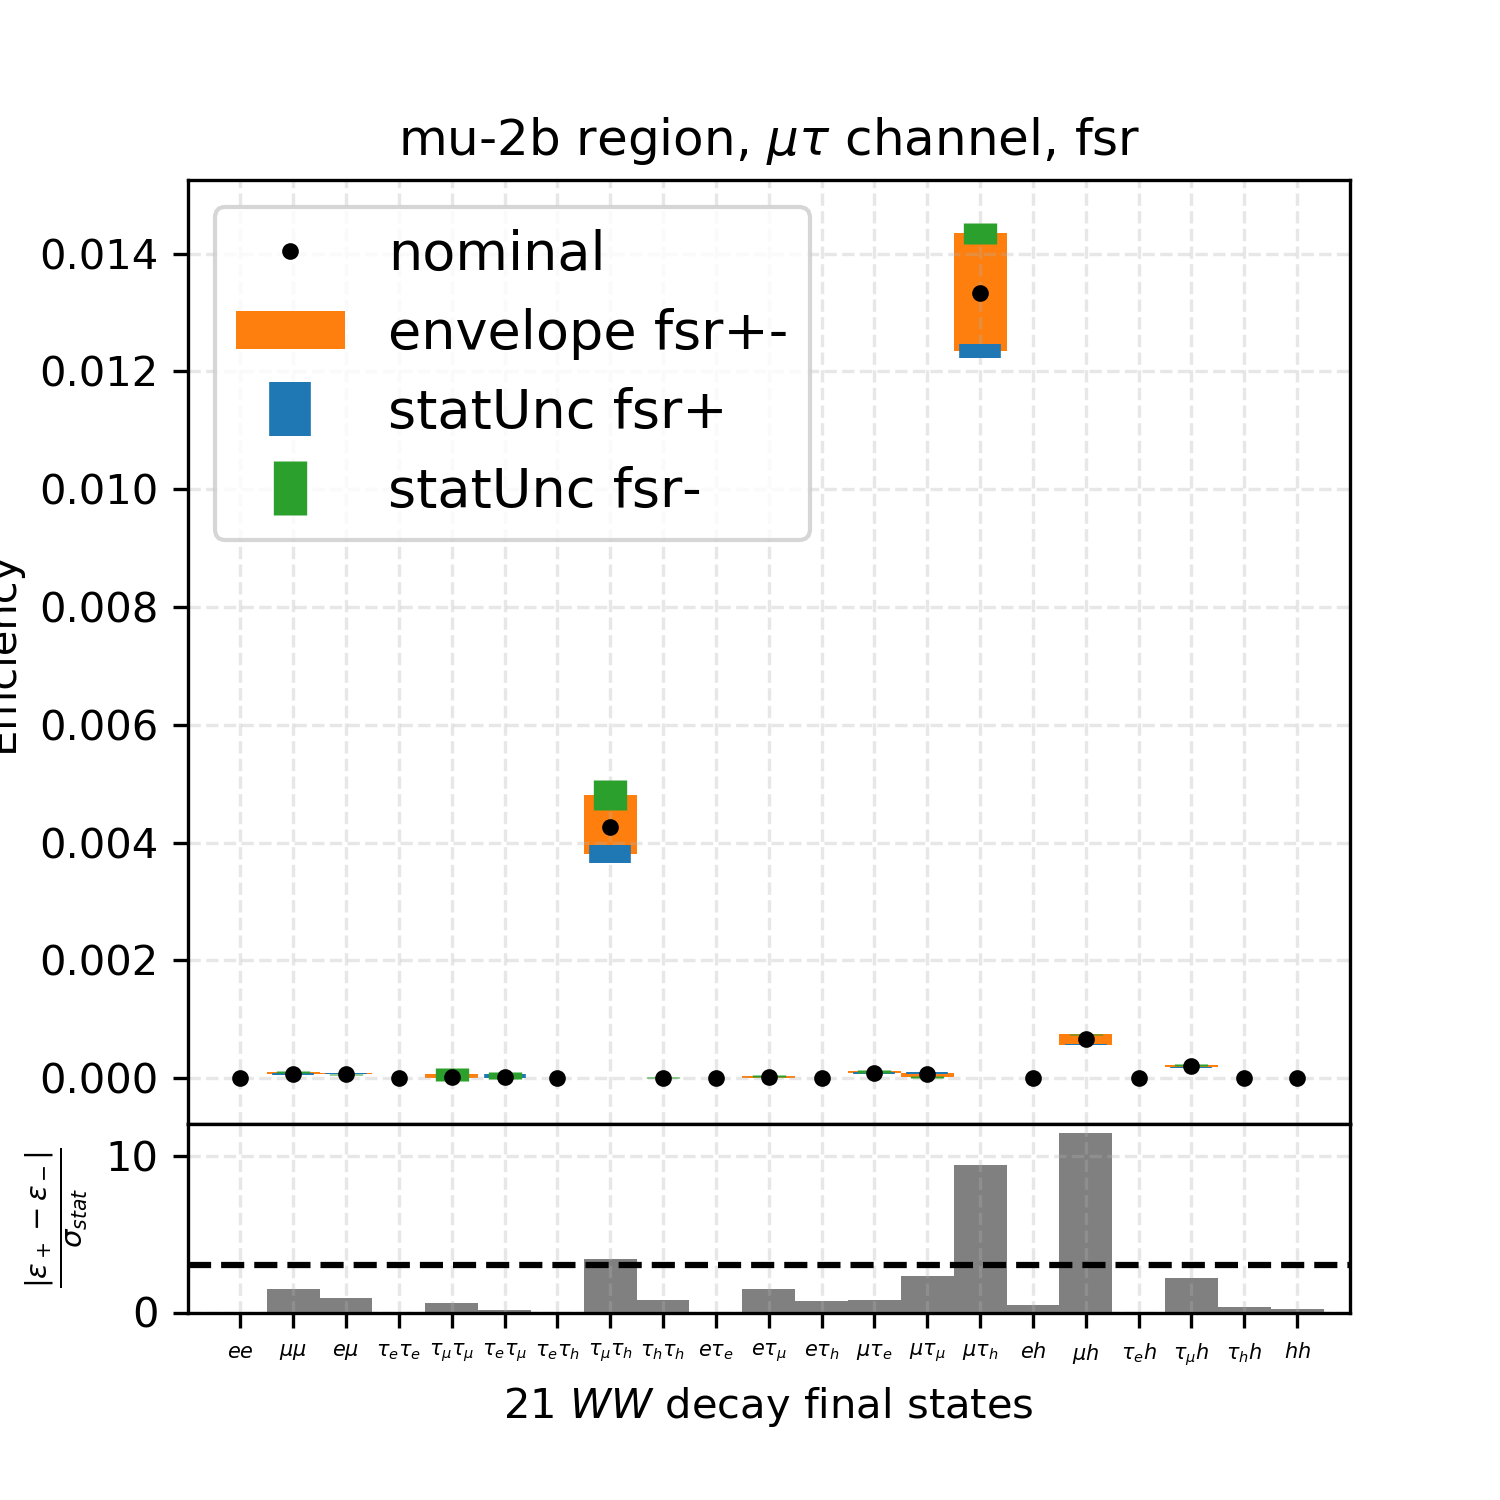
\includegraphics[width=0.24\textwidth]{chapters/Appendix/sectionTTSyst/figures/afterCorr/icata1_ch2_fsr.png}
    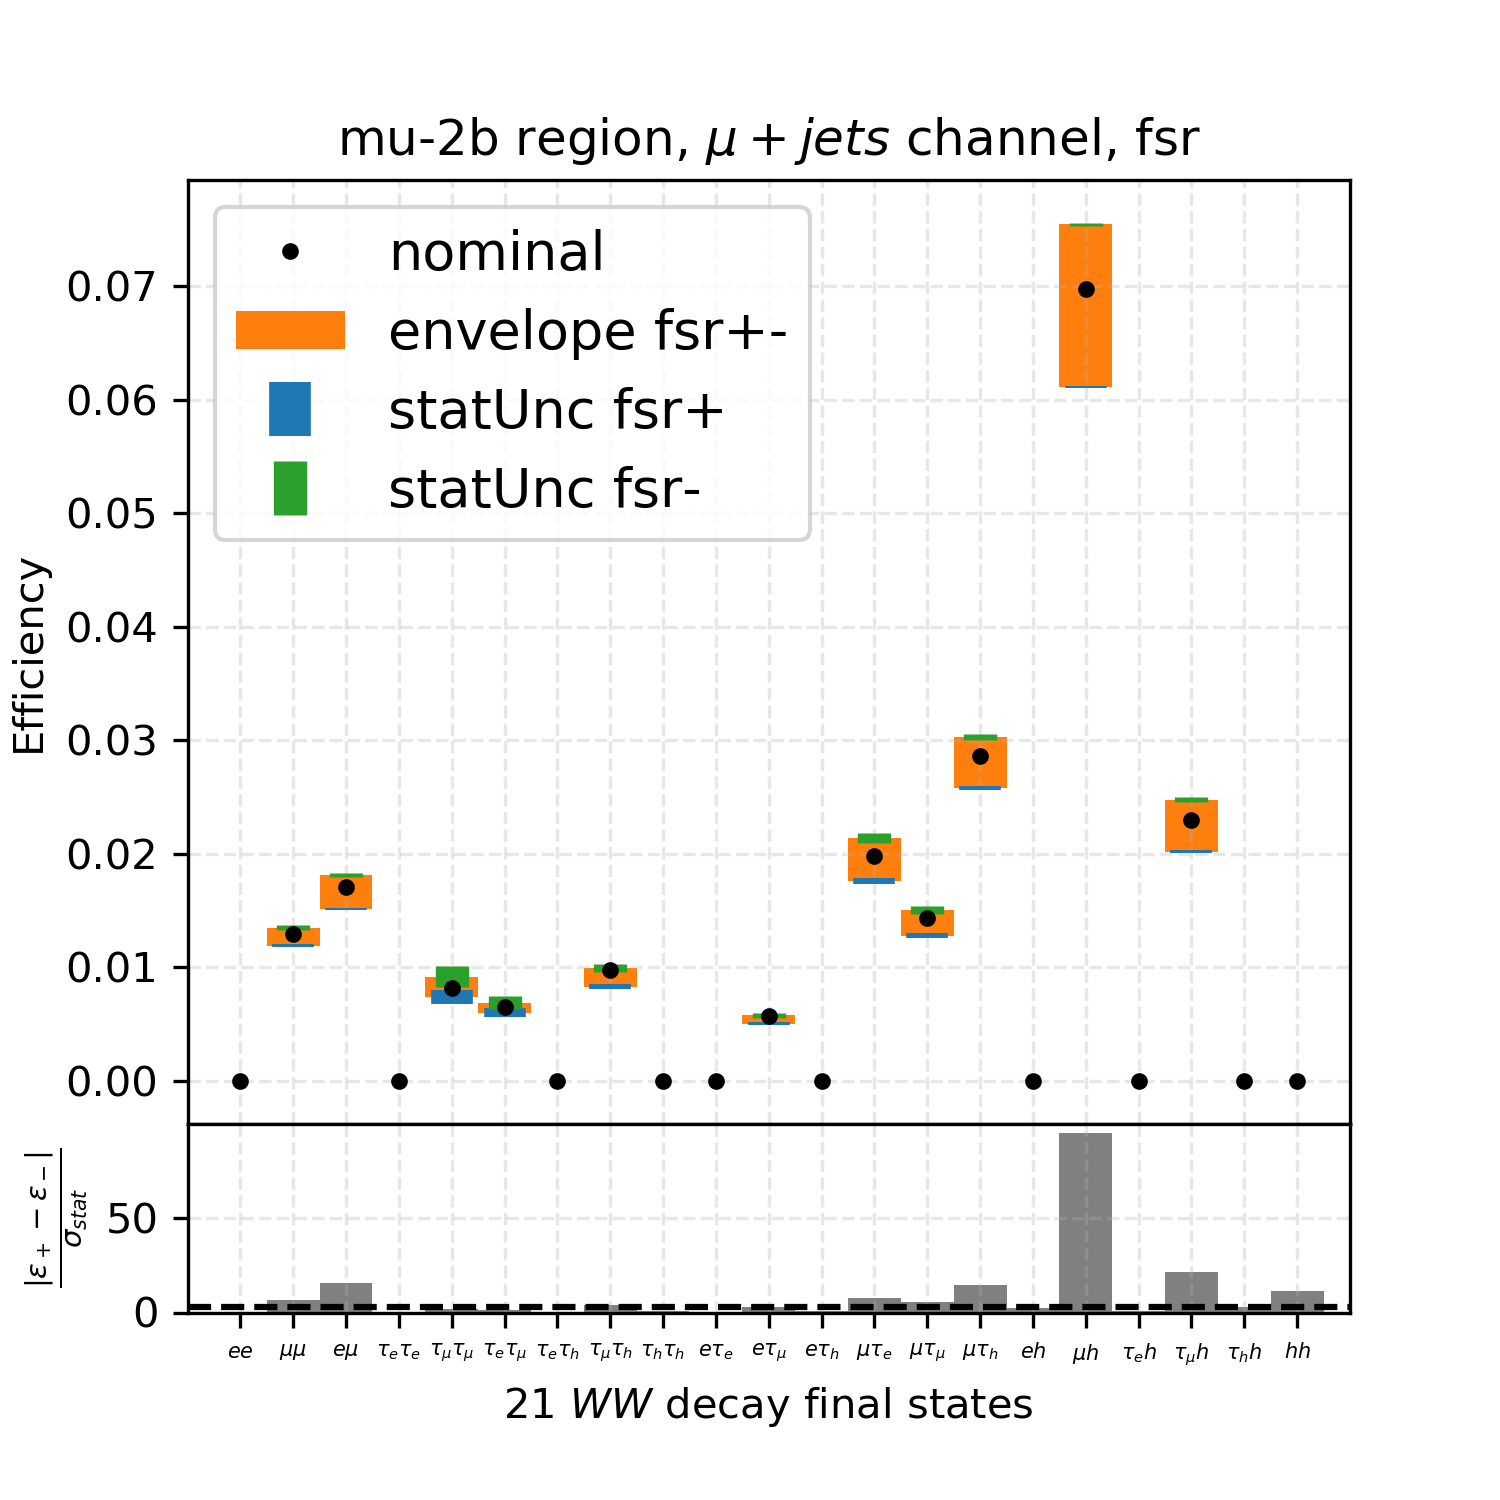
\includegraphics[width=0.24\textwidth]{chapters/Appendix/sectionTTSyst/figures/afterCorr/icata1_ch3_fsr.png}
    
    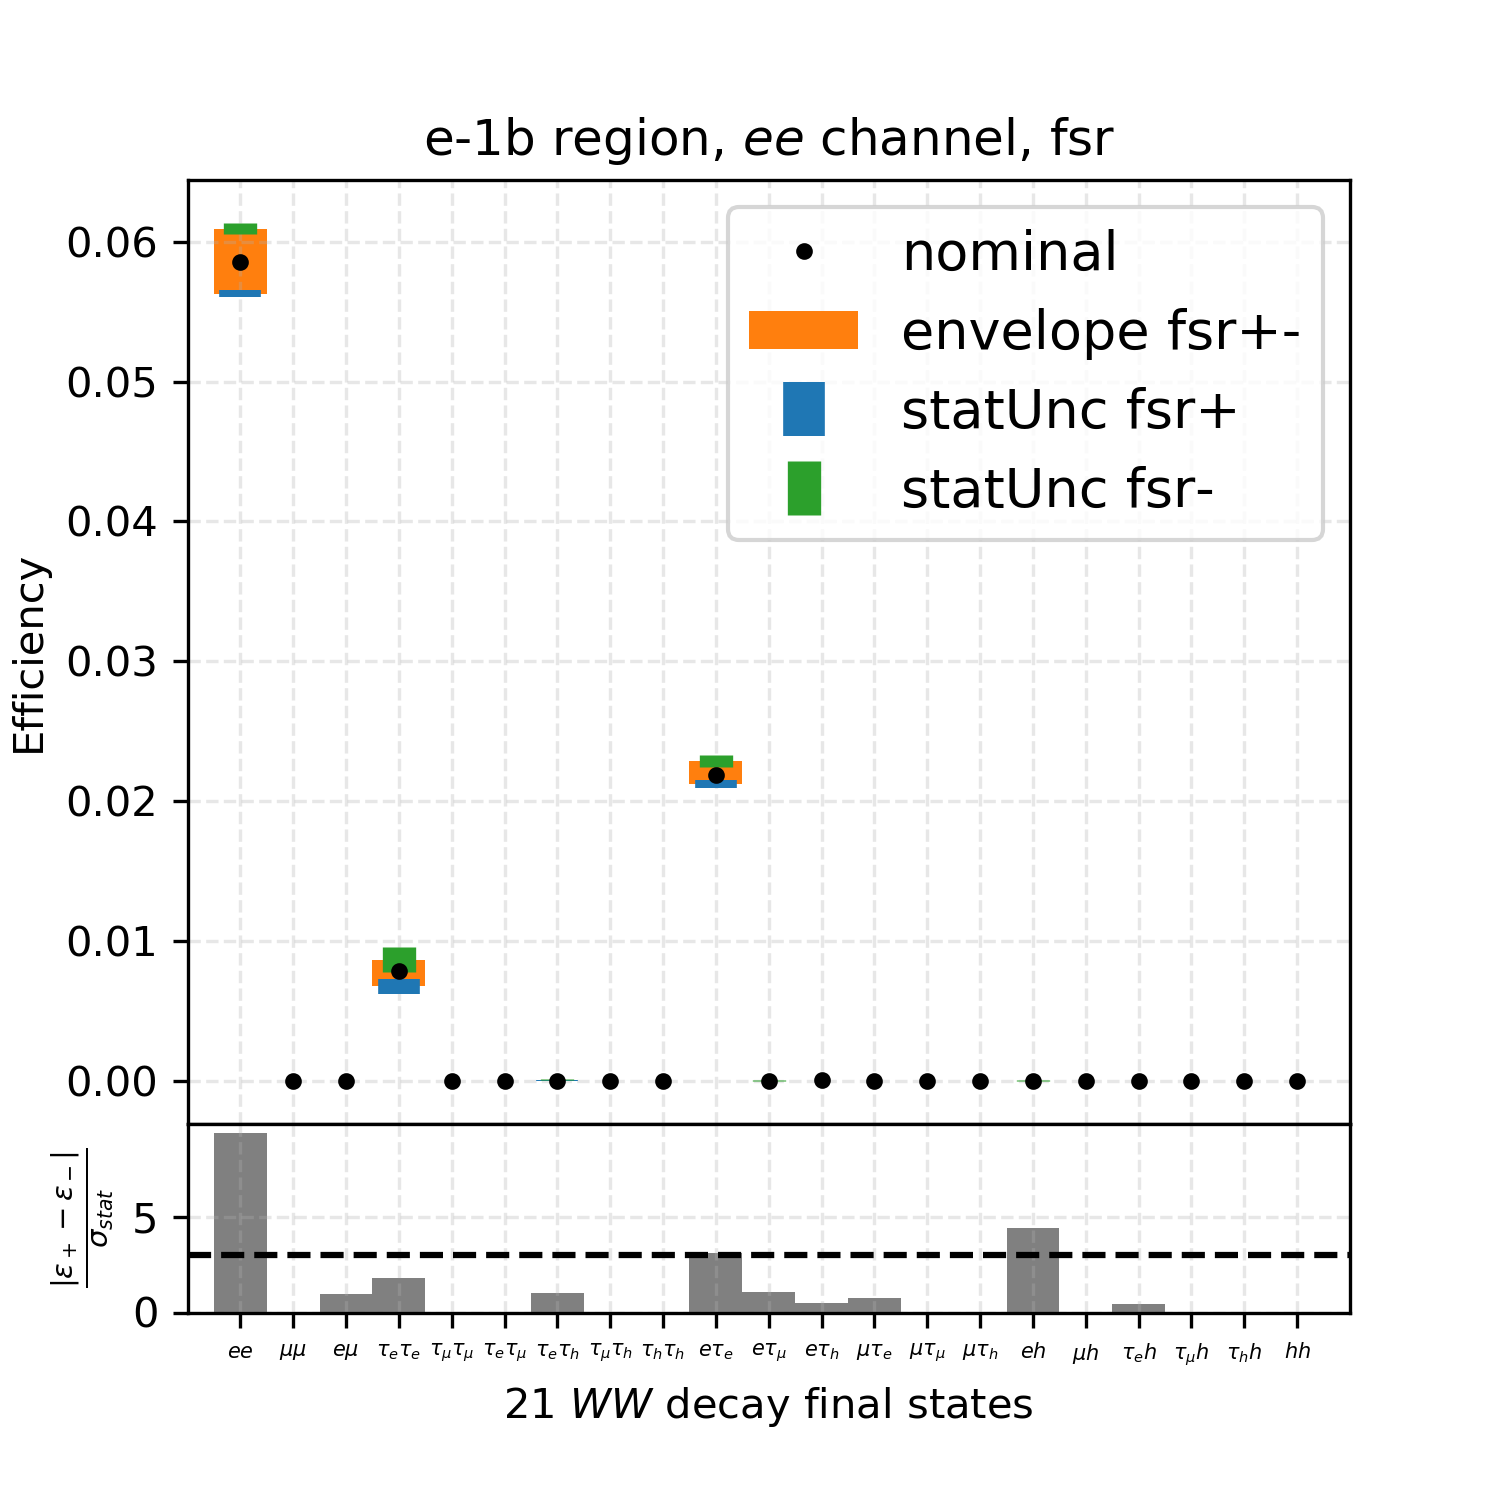
\includegraphics[width=0.24\textwidth]{chapters/Appendix/sectionTTSyst/figures/afterCorr/icata2_ch0_fsr.png}
    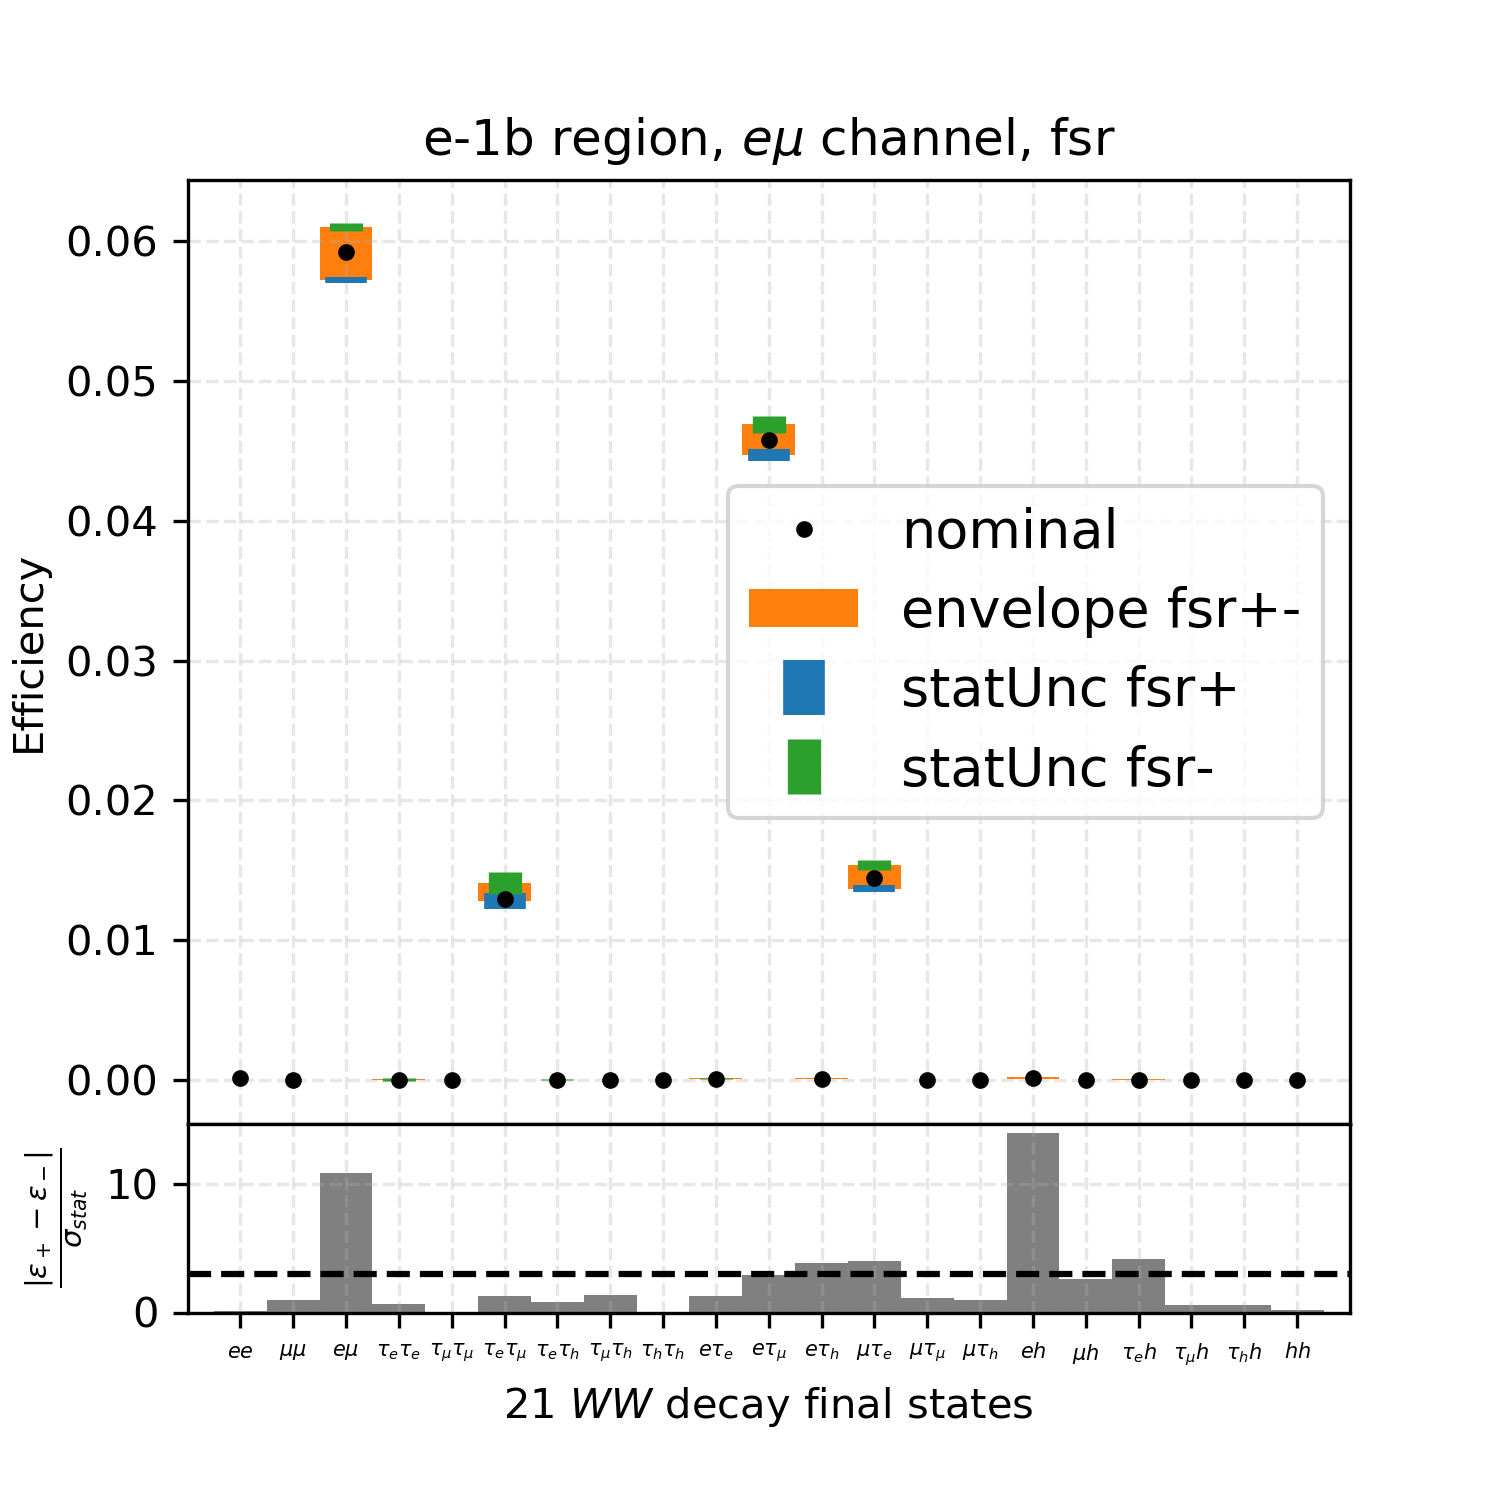
\includegraphics[width=0.24\textwidth]{chapters/Appendix/sectionTTSyst/figures/afterCorr/icata2_ch1_fsr.png}
    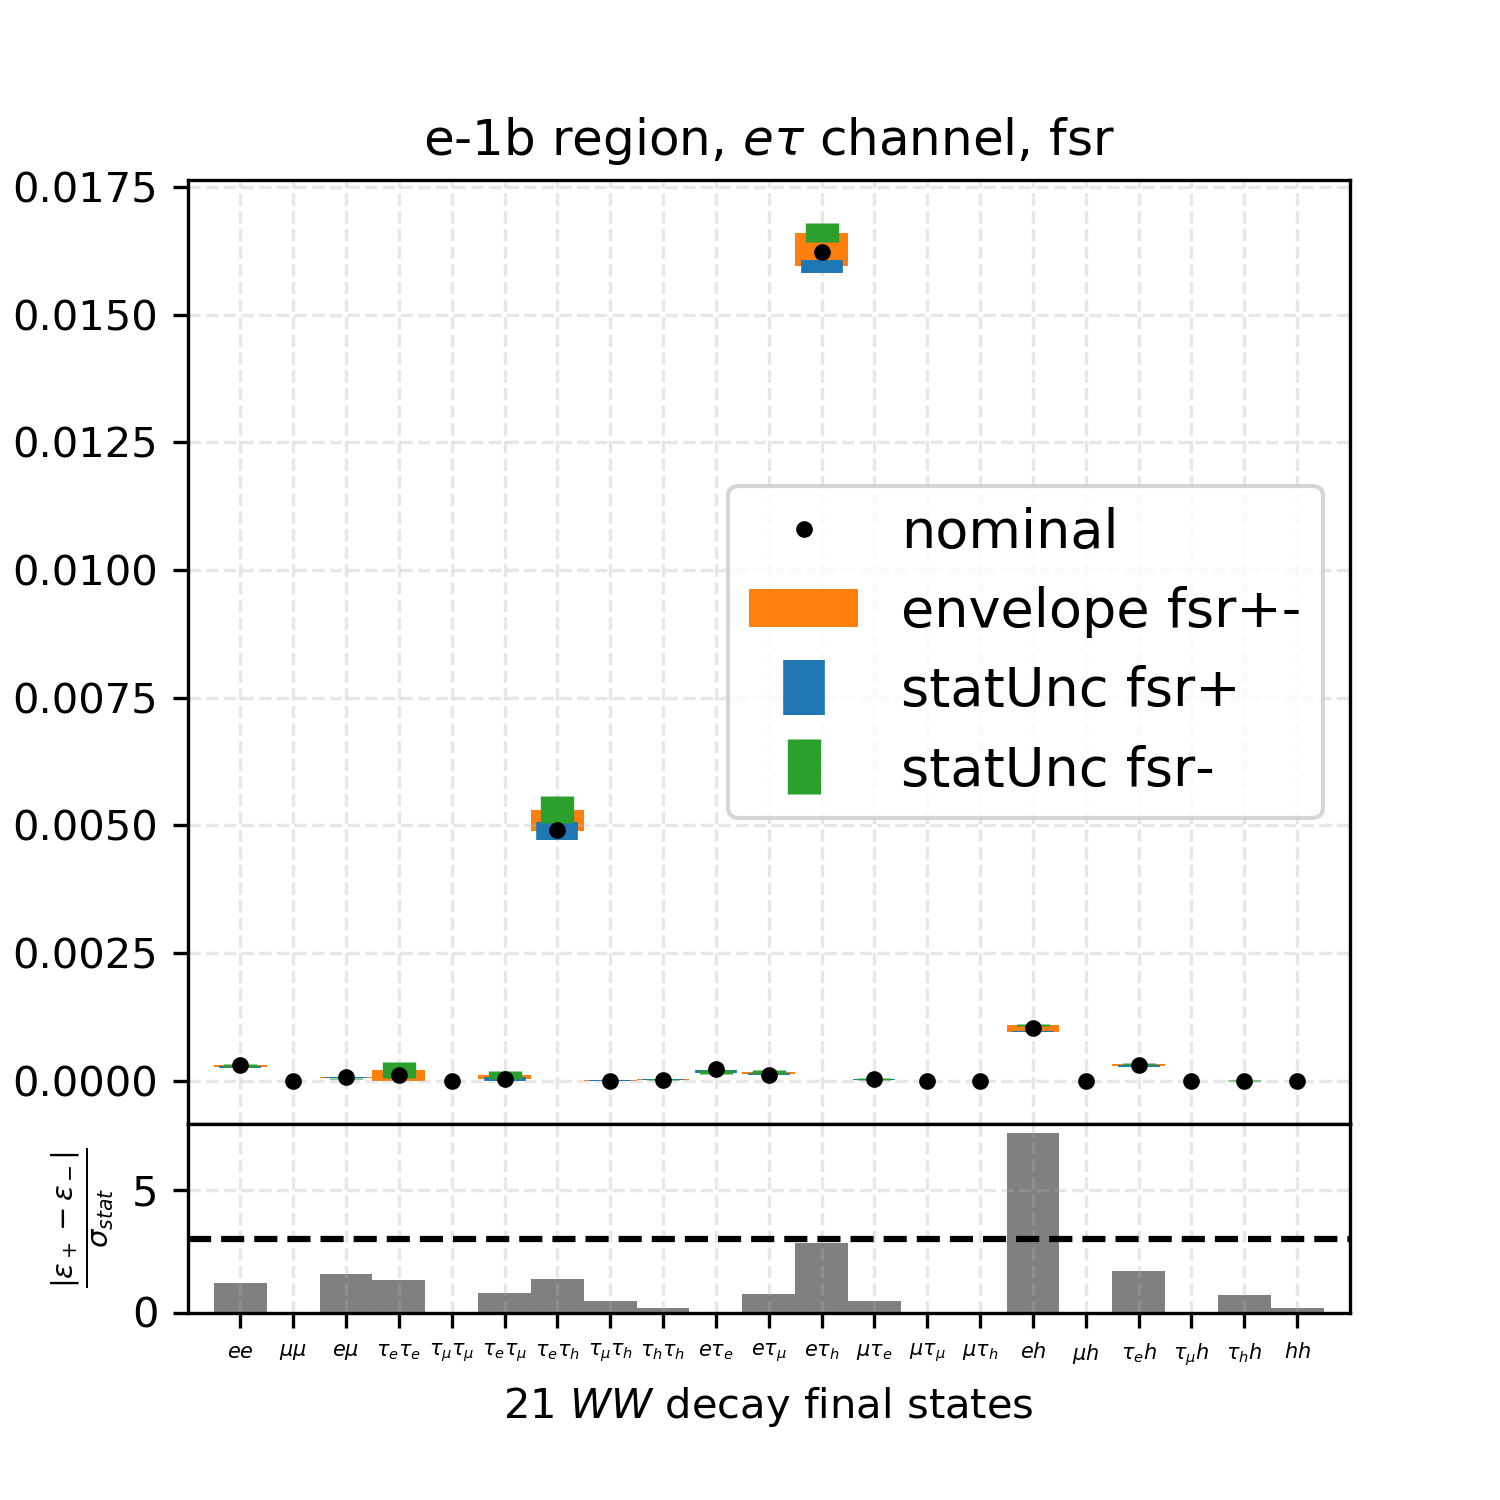
\includegraphics[width=0.24\textwidth]{chapters/Appendix/sectionTTSyst/figures/afterCorr/icata2_ch2_fsr.png}
    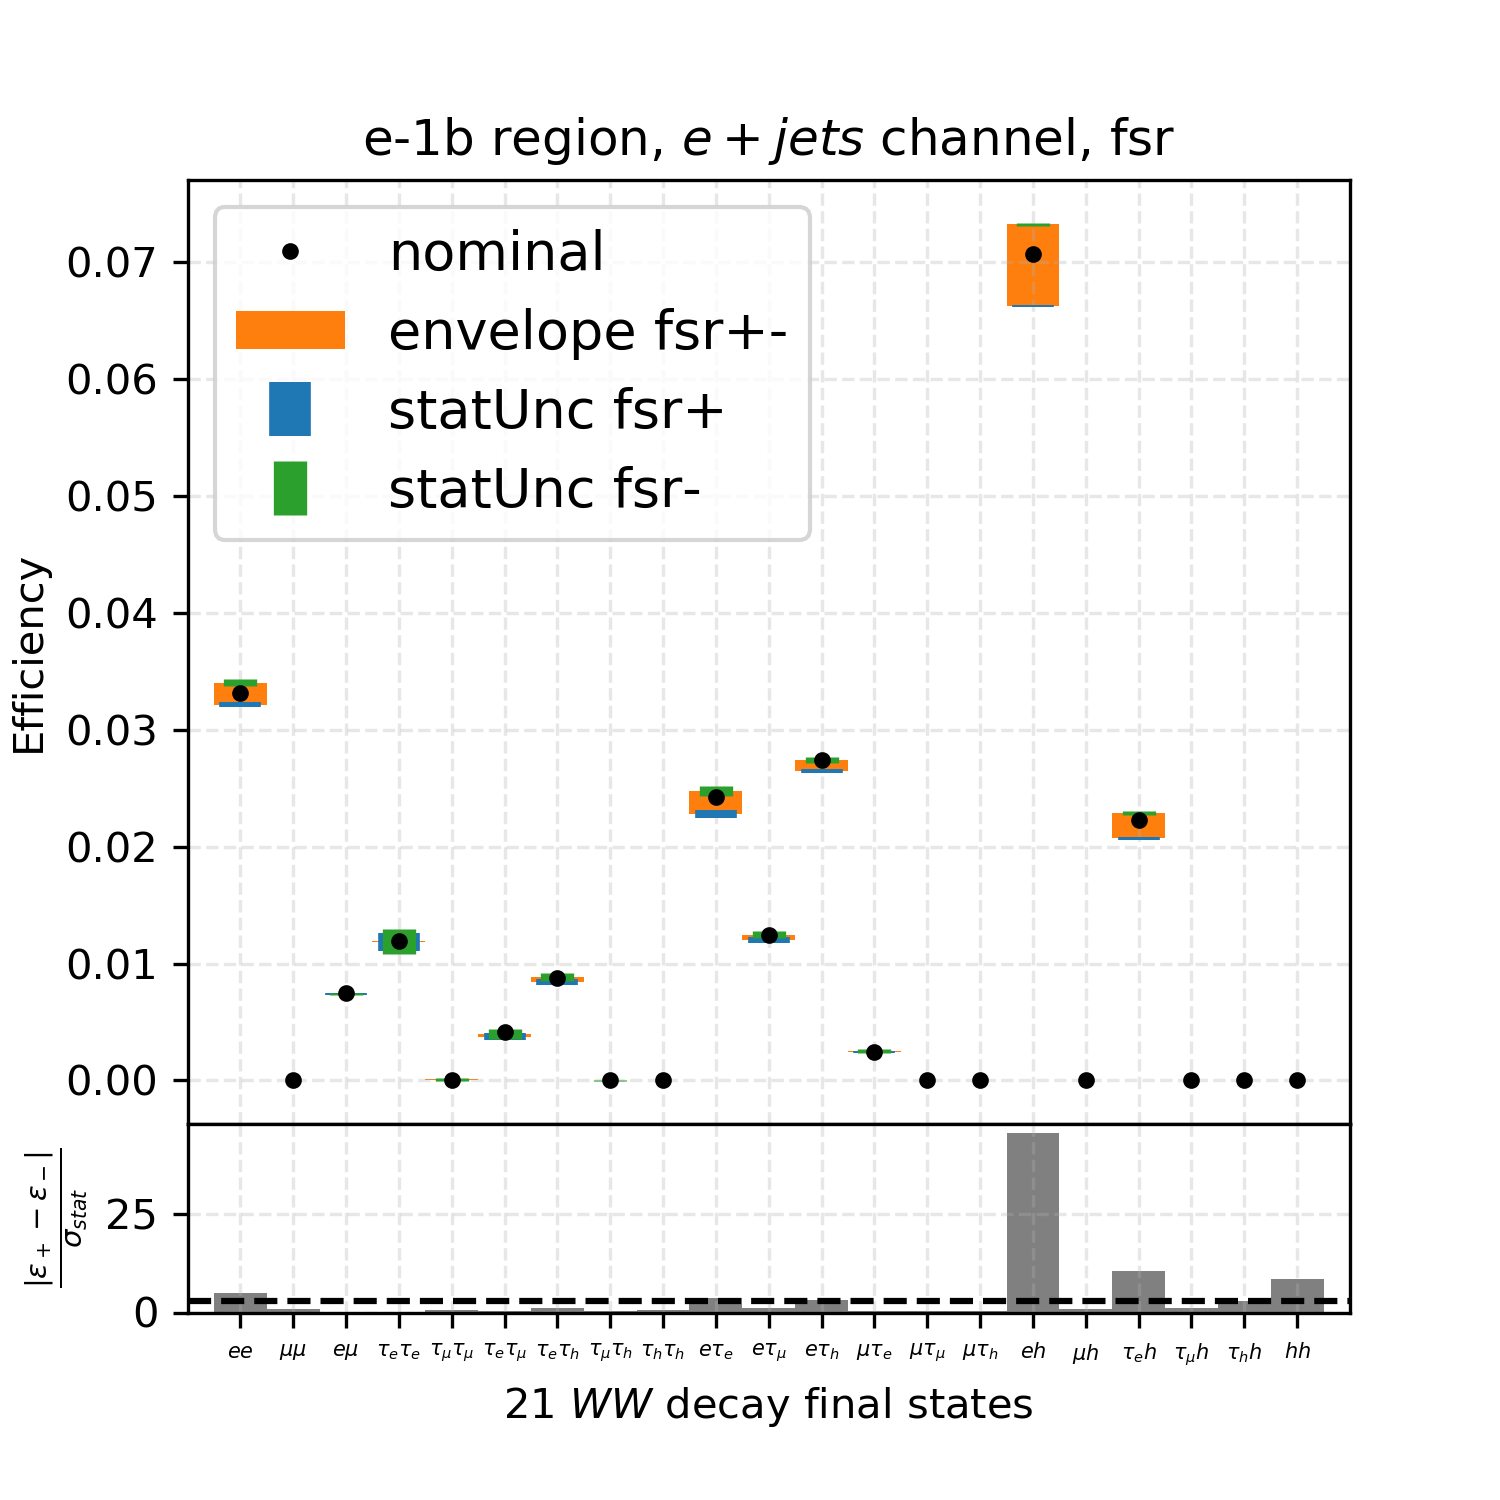
\includegraphics[width=0.24\textwidth]{chapters/Appendix/sectionTTSyst/figures/afterCorr/icata2_ch3_fsr.png}

    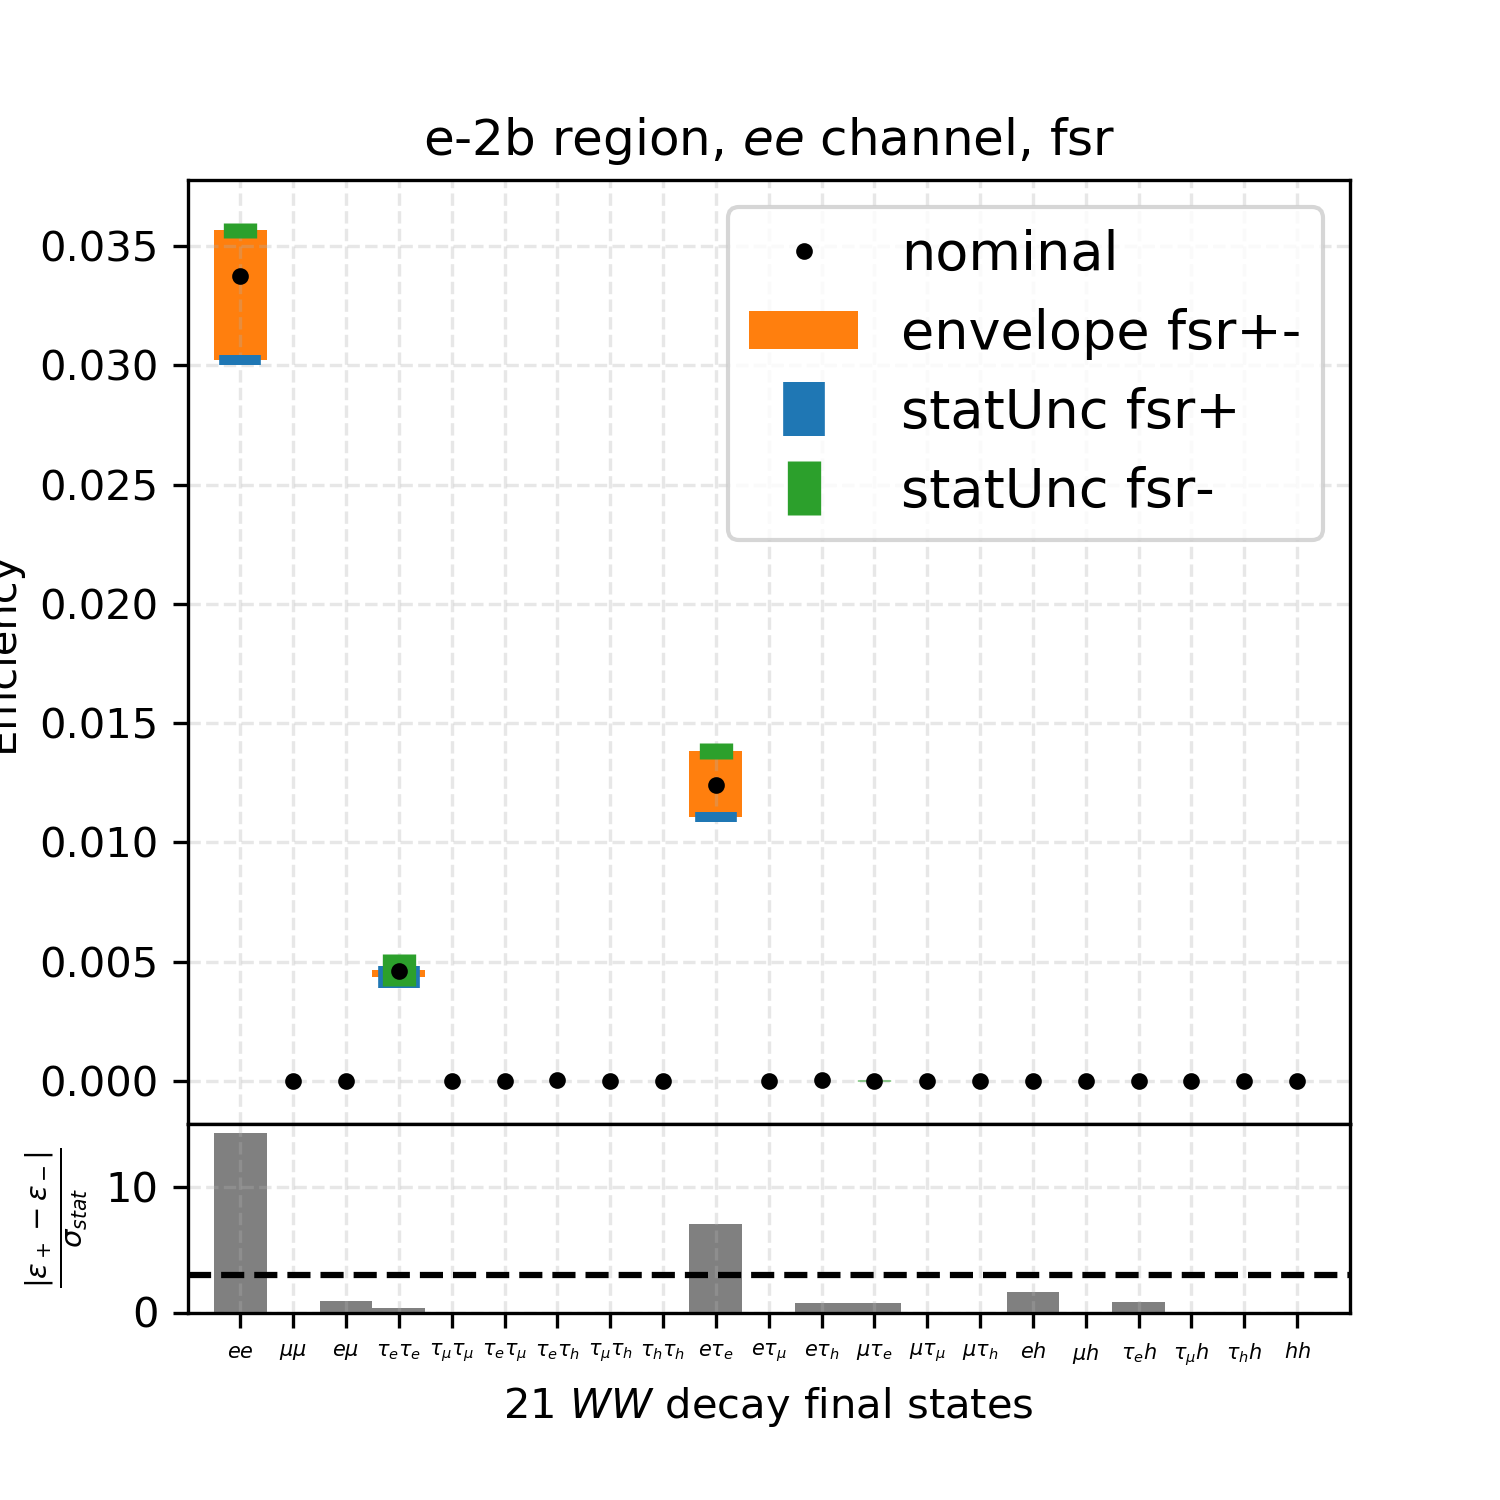
\includegraphics[width=0.24\textwidth]{chapters/Appendix/sectionTTSyst/figures/afterCorr/icata3_ch0_fsr.png}
    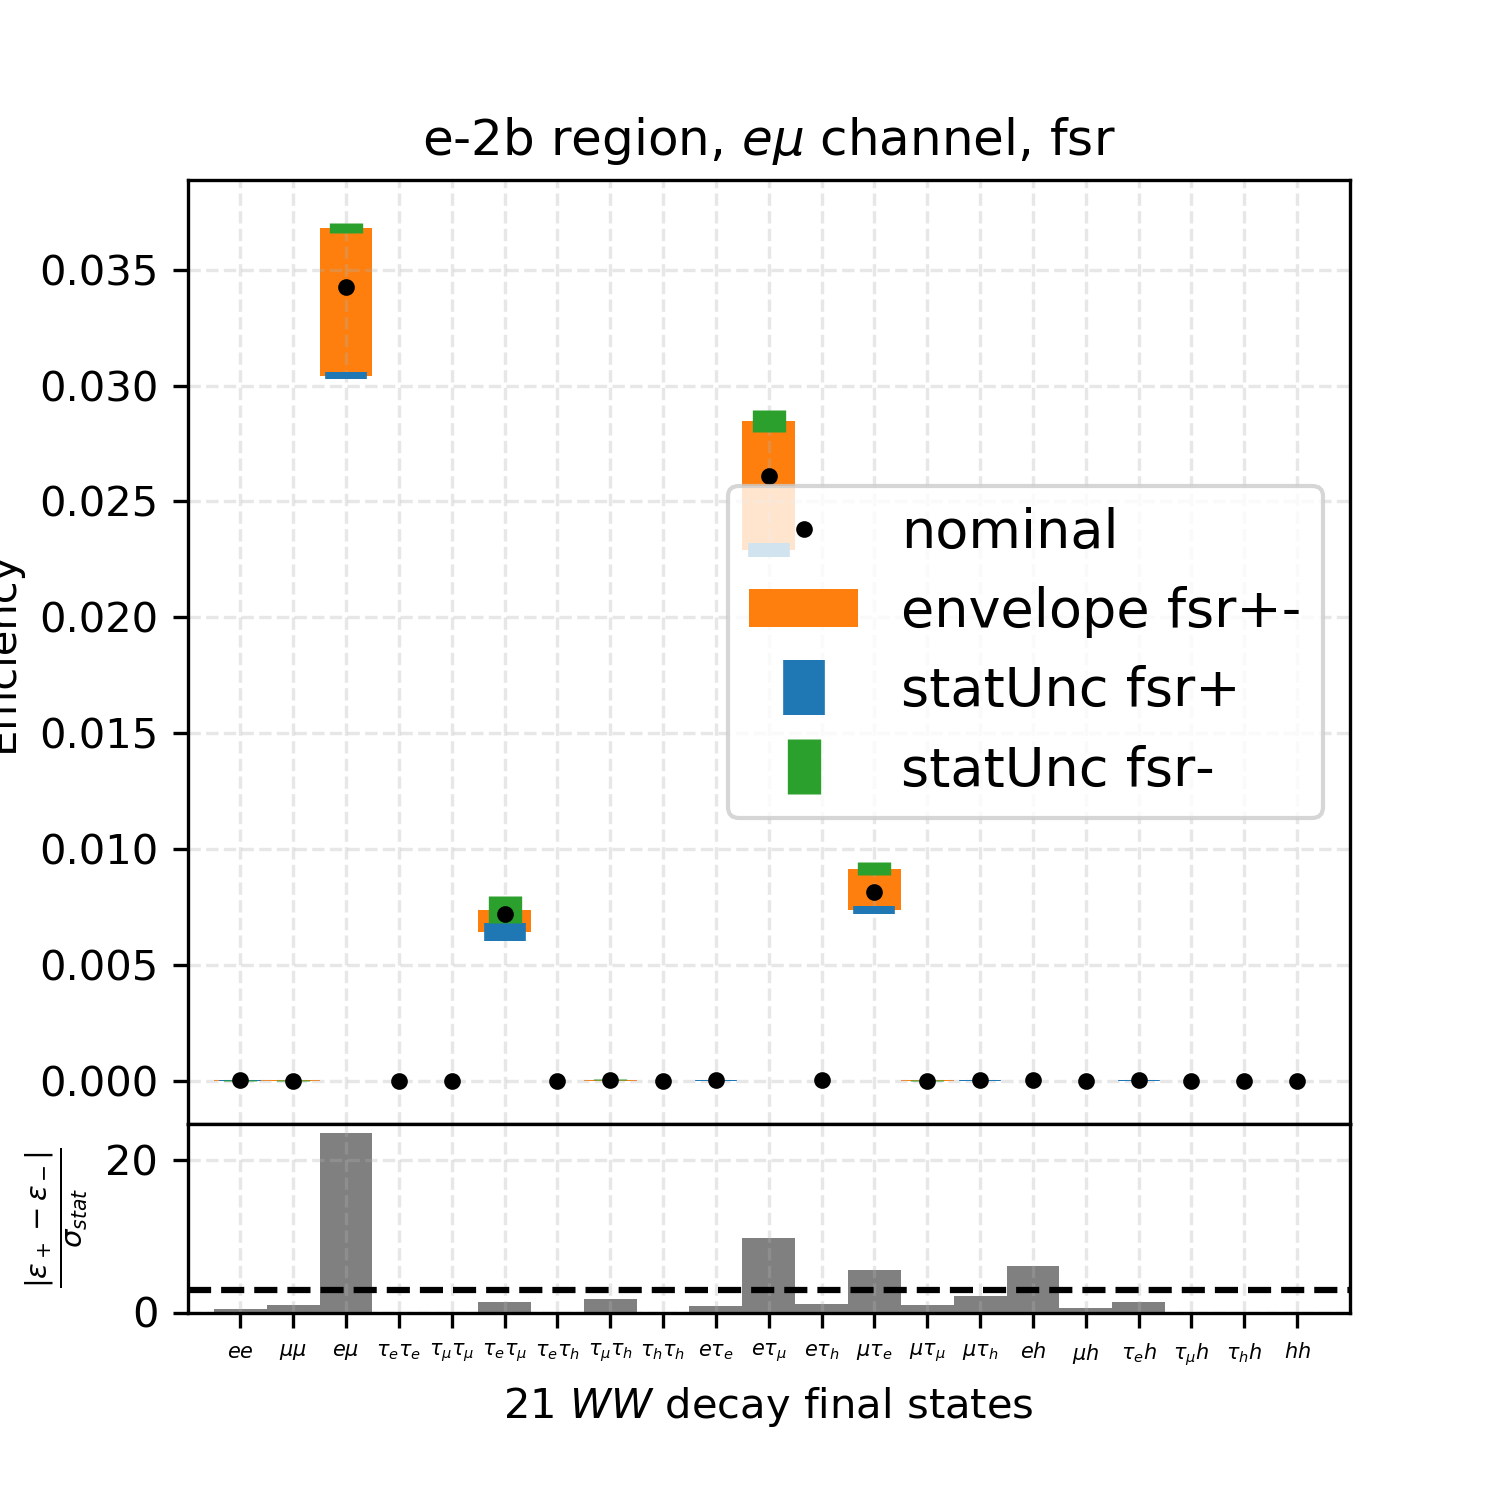
\includegraphics[width=0.24\textwidth]{chapters/Appendix/sectionTTSyst/figures/afterCorr/icata3_ch1_fsr.png}
    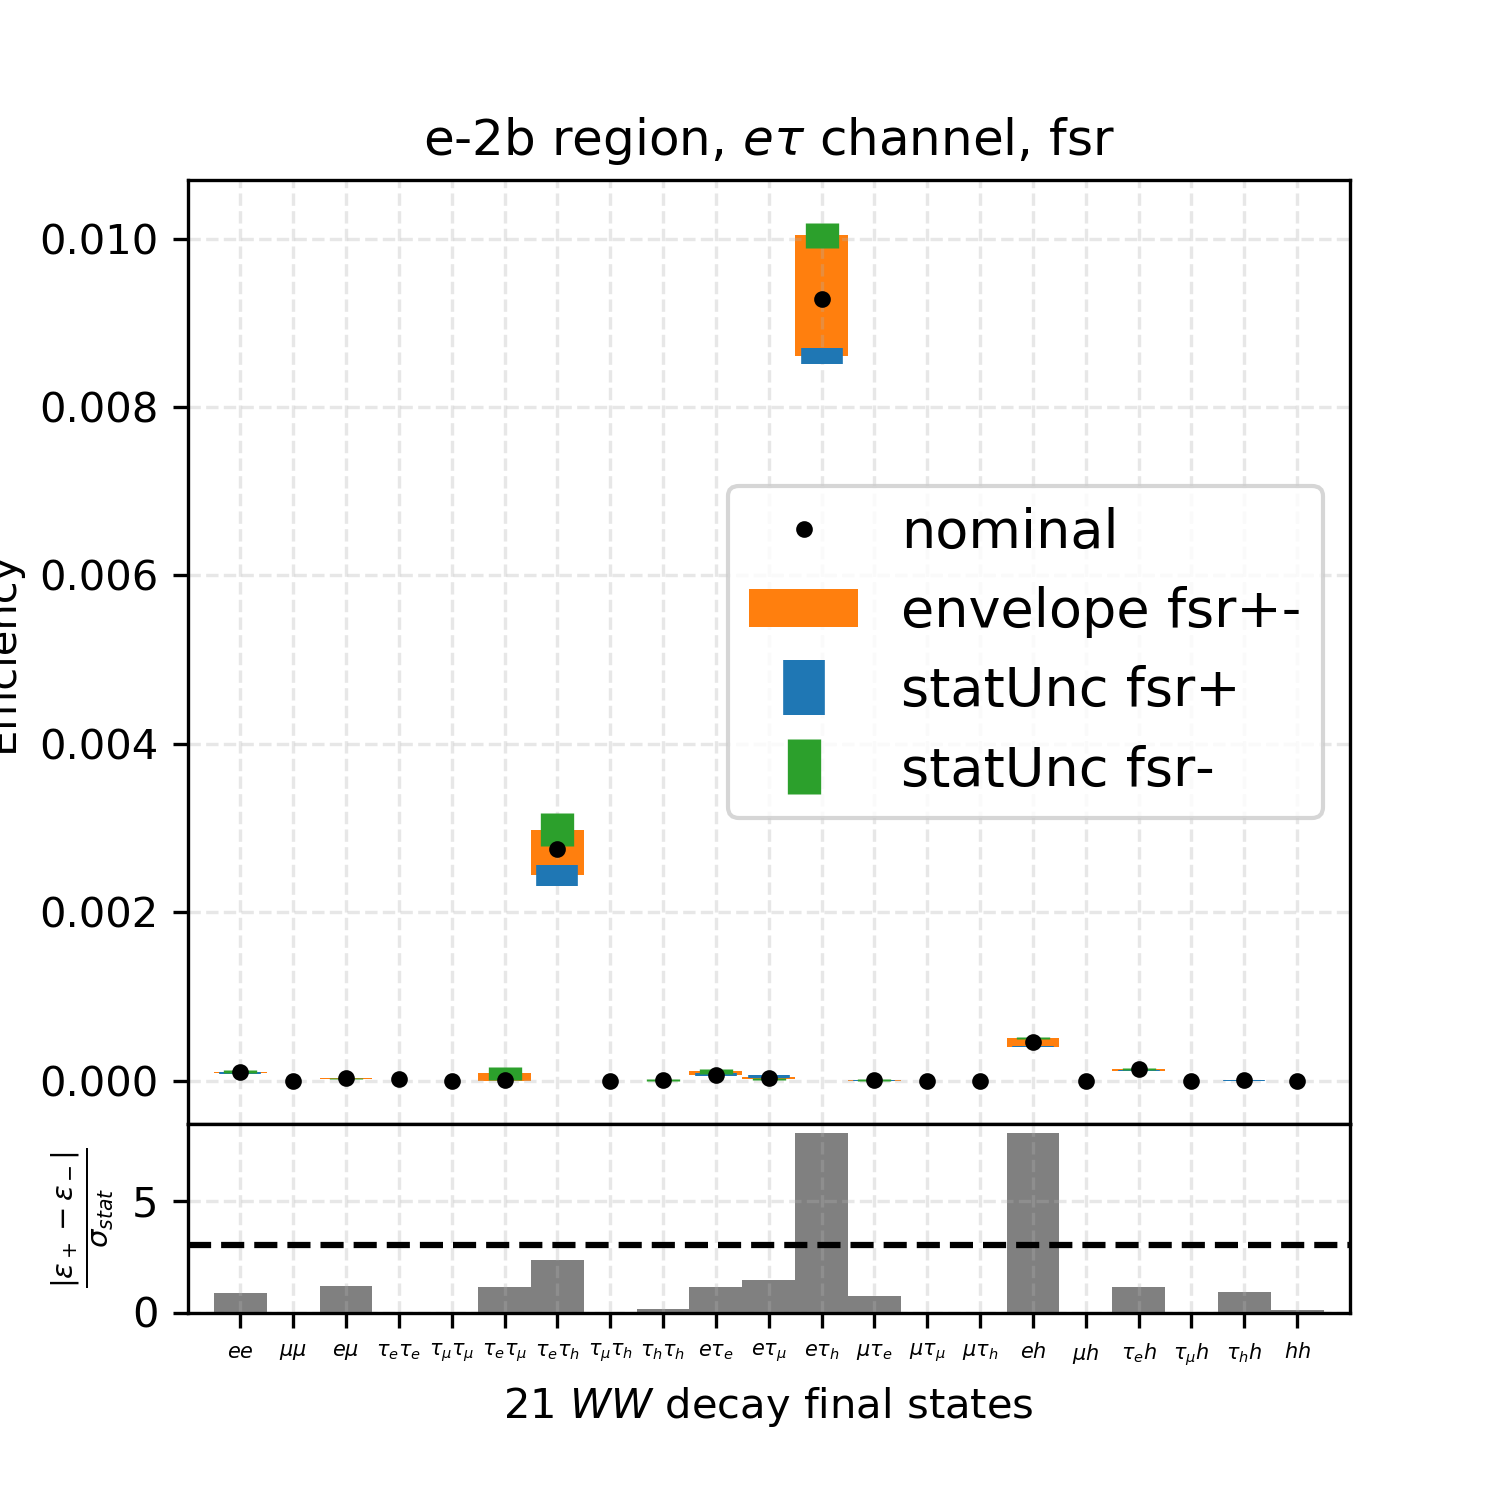
\includegraphics[width=0.24\textwidth]{chapters/Appendix/sectionTTSyst/figures/afterCorr/icata3_ch2_fsr.png}
    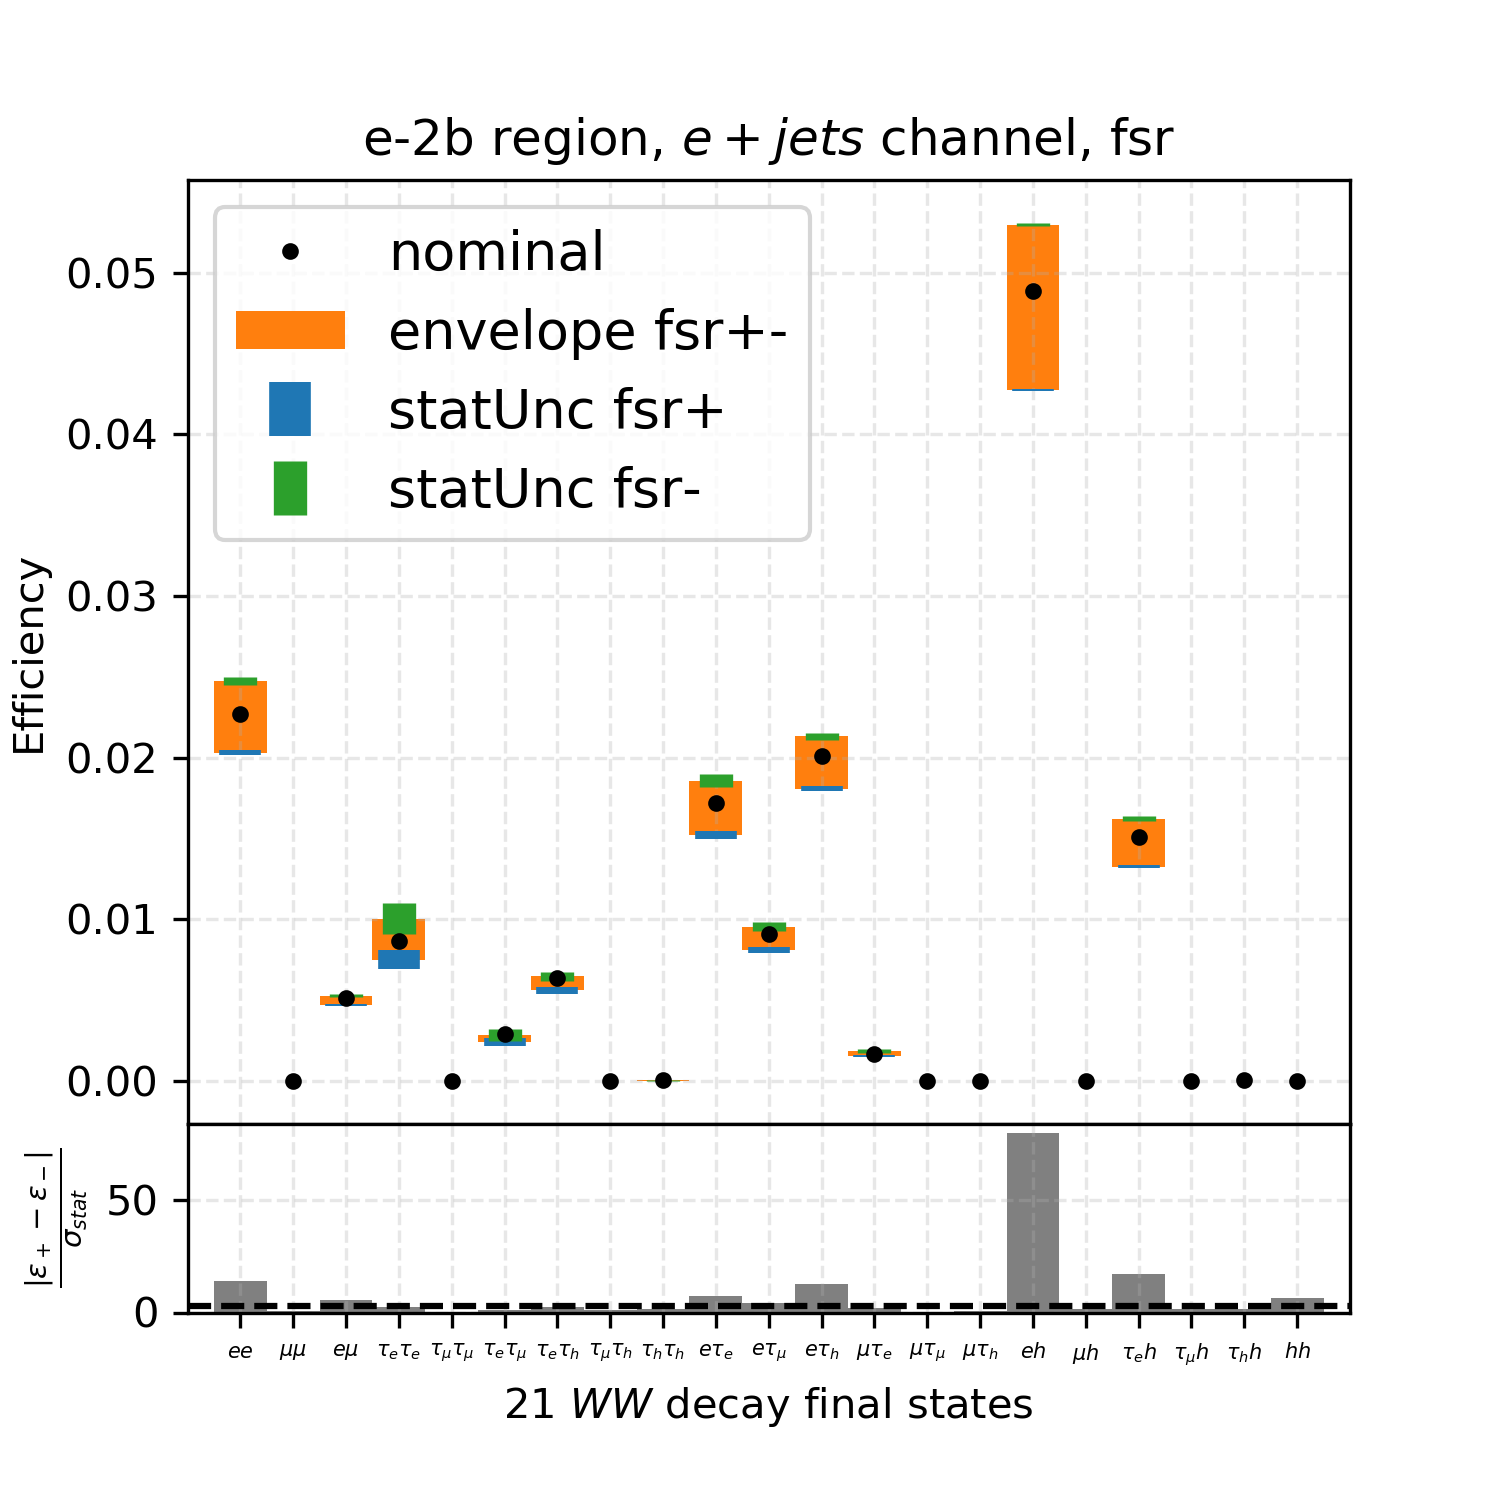
\includegraphics[width=0.24\textwidth]{chapters/Appendix/sectionTTSyst/figures/afterCorr/icata3_ch3_fsr.png}
    
    \caption{FSR envelops on 21 efficiencies. VTight WP is shown.}
    \label{fig:appendix:reweighttt:effAfterCorrFSR}
\end{figure}



\begin{figure}
    \centering
    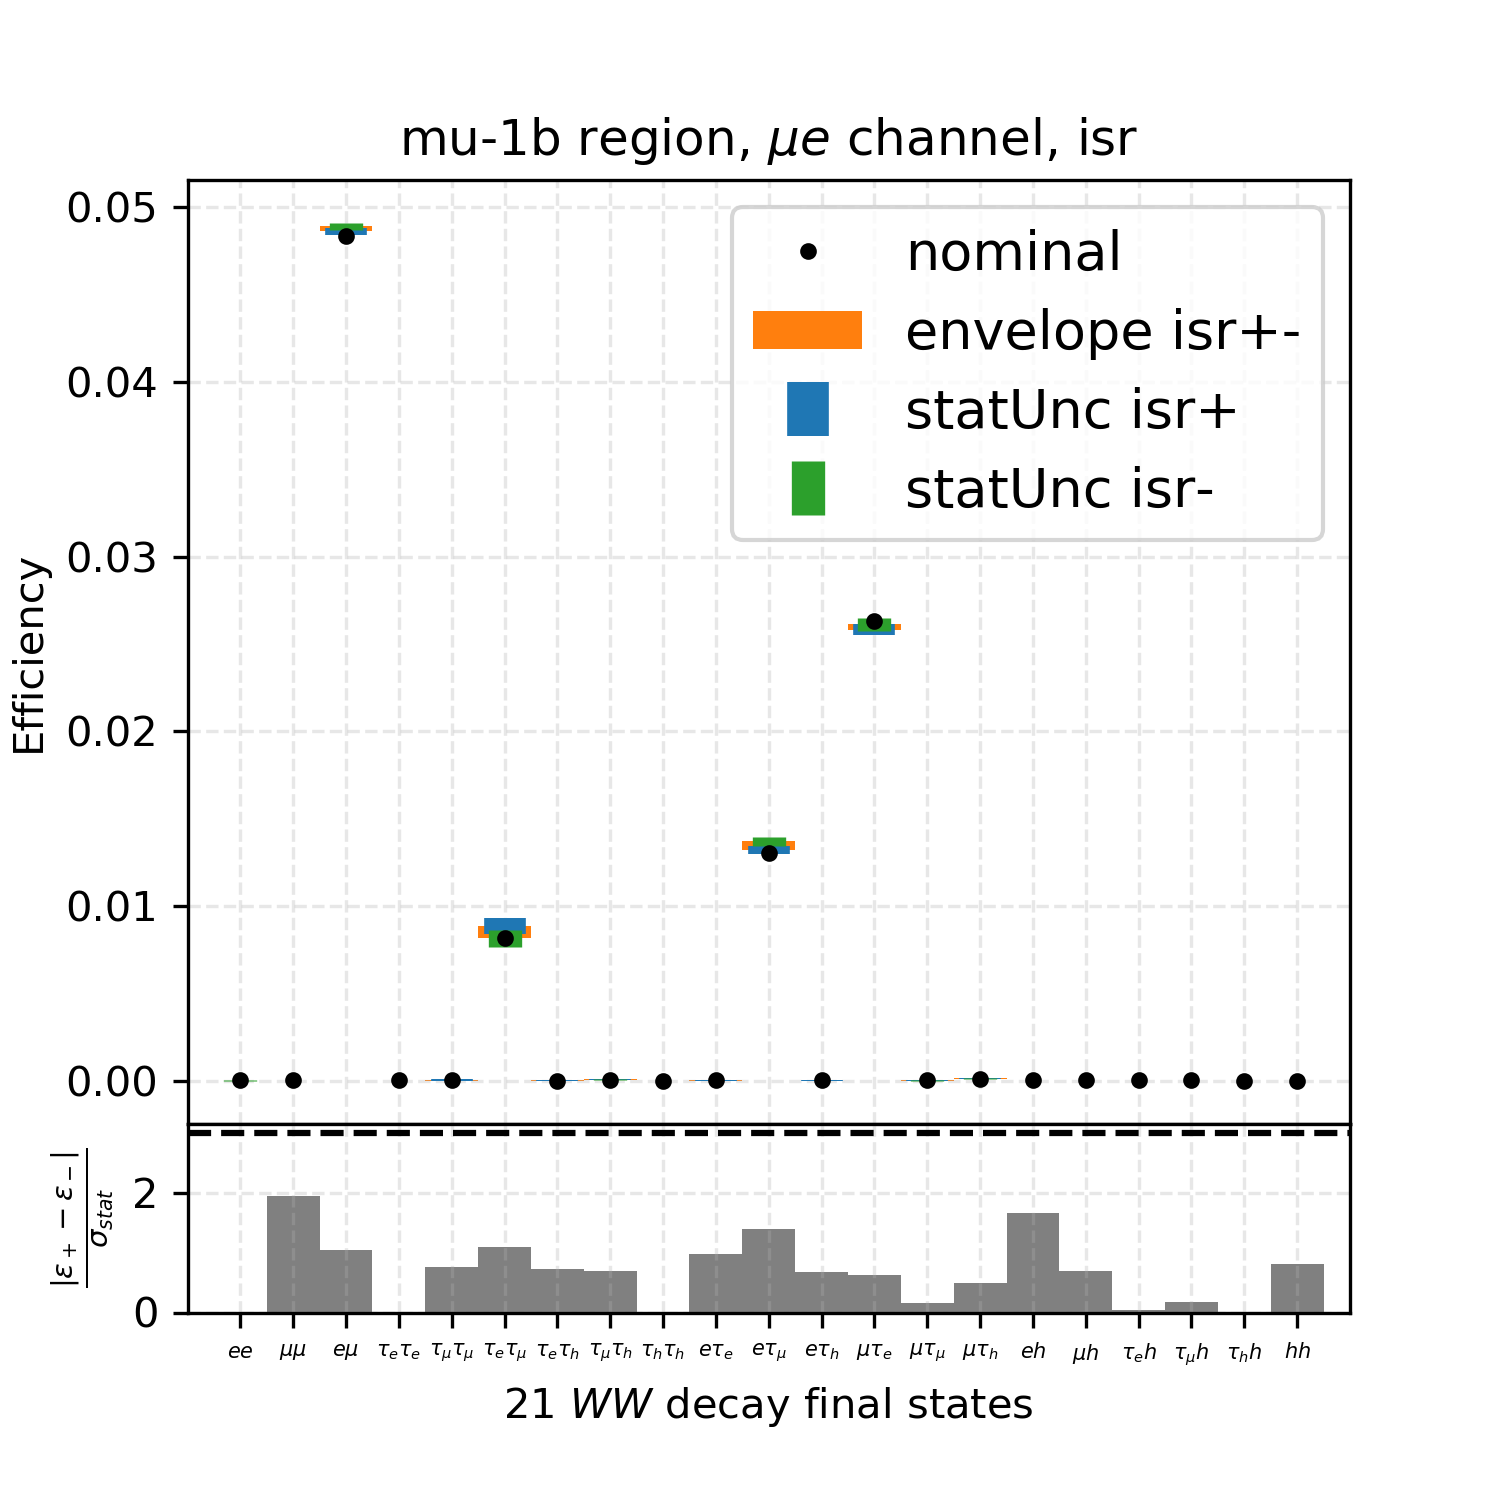
\includegraphics[width=0.24\textwidth]{chapters/Appendix/sectionTTSyst/figures/afterCorr/icata0_ch0_isr.png}
    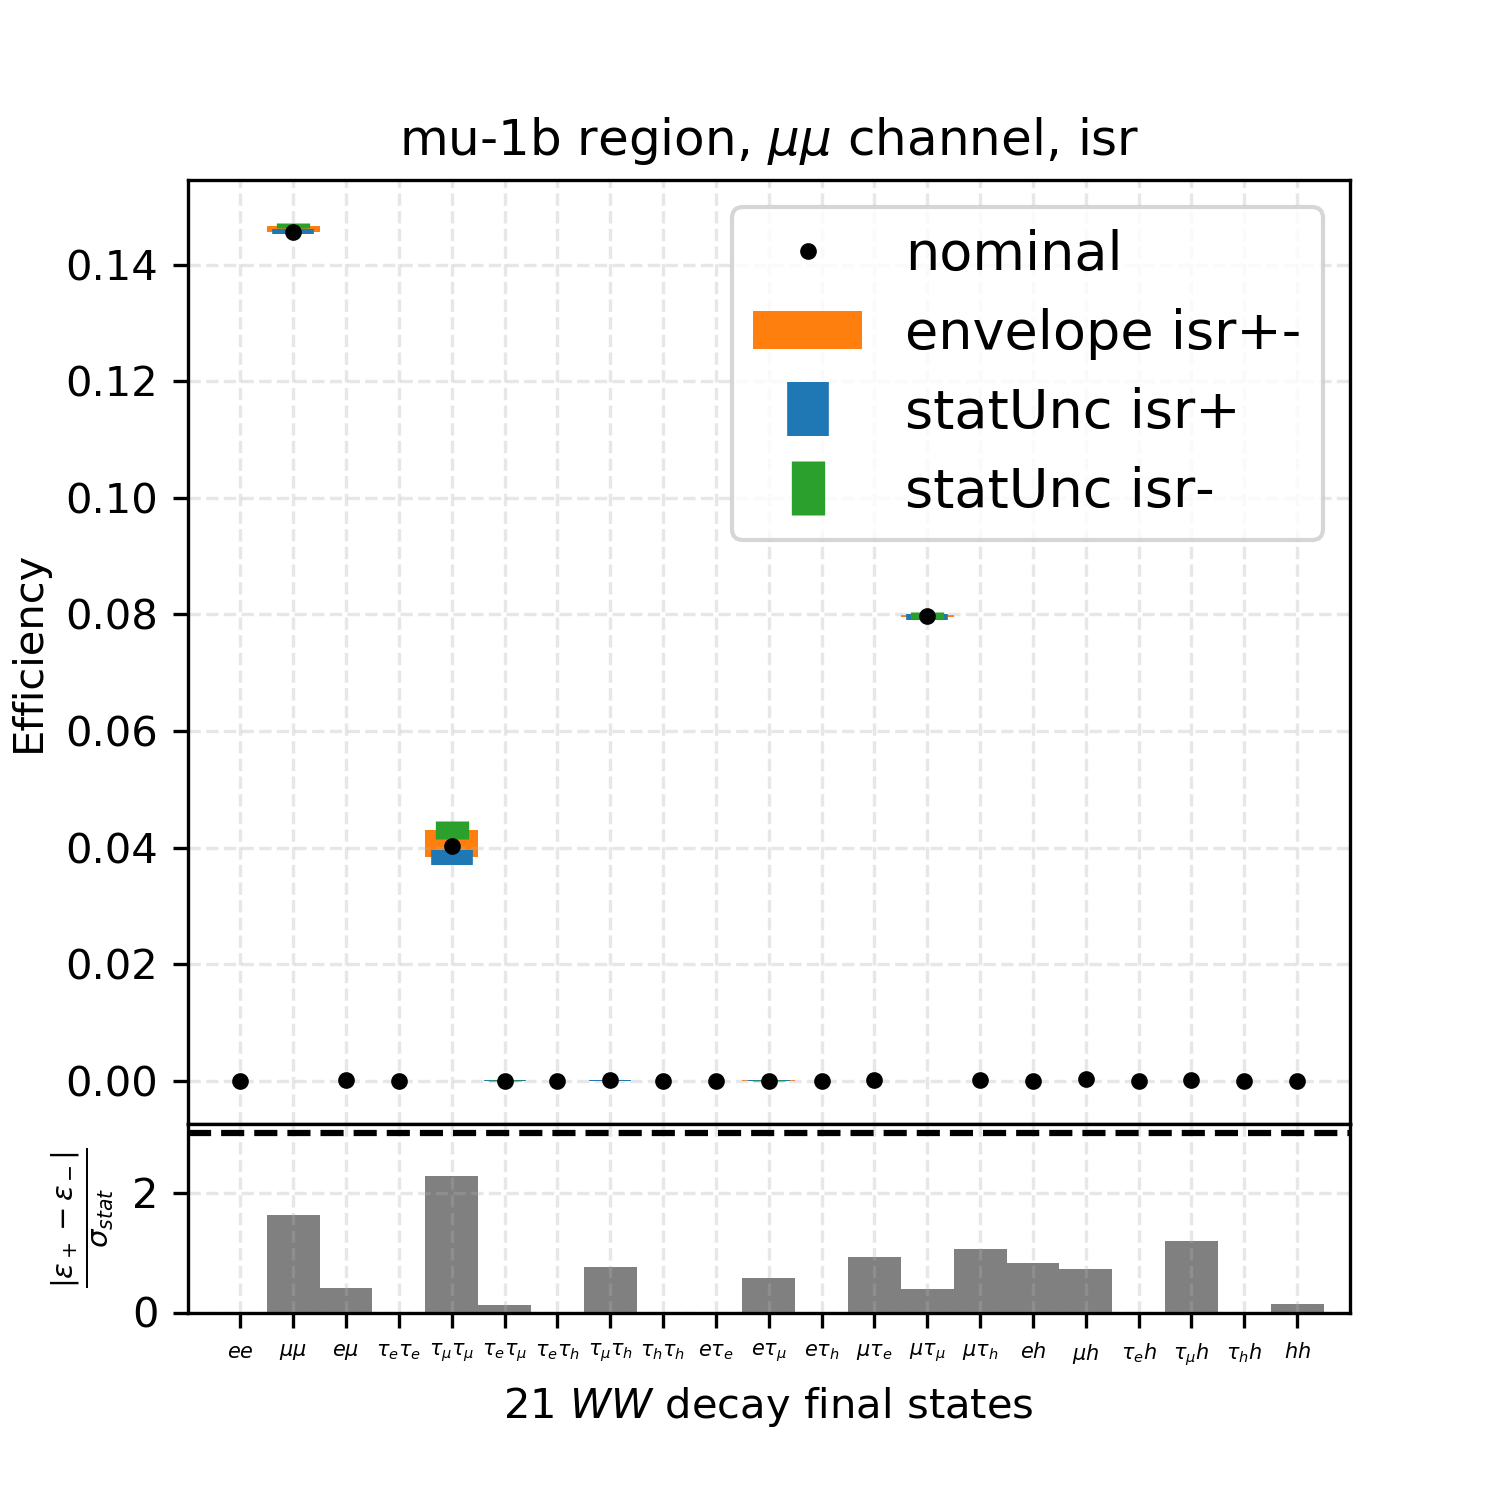
\includegraphics[width=0.24\textwidth]{chapters/Appendix/sectionTTSyst/figures/afterCorr/icata0_ch1_isr.png}
    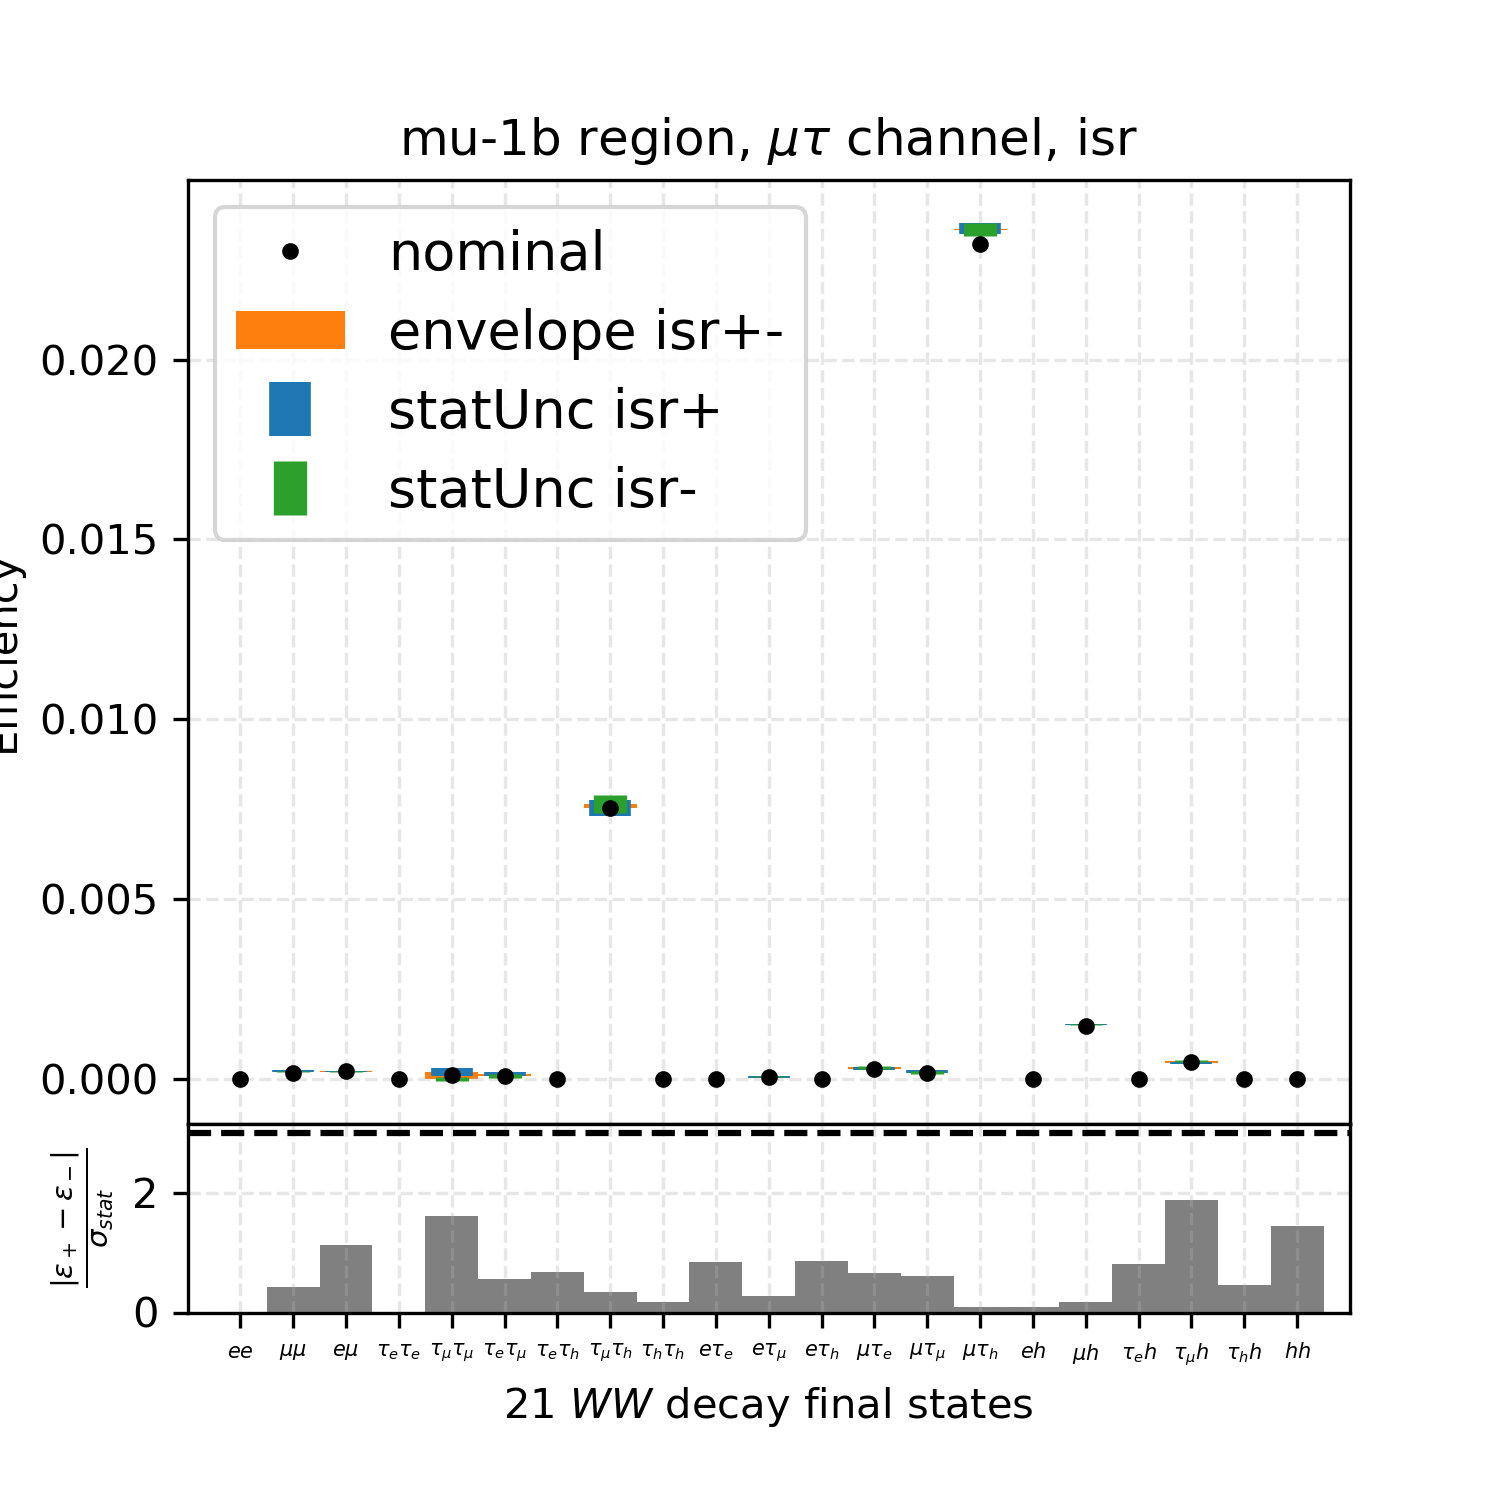
\includegraphics[width=0.24\textwidth]{chapters/Appendix/sectionTTSyst/figures/afterCorr/icata0_ch2_isr.png}
    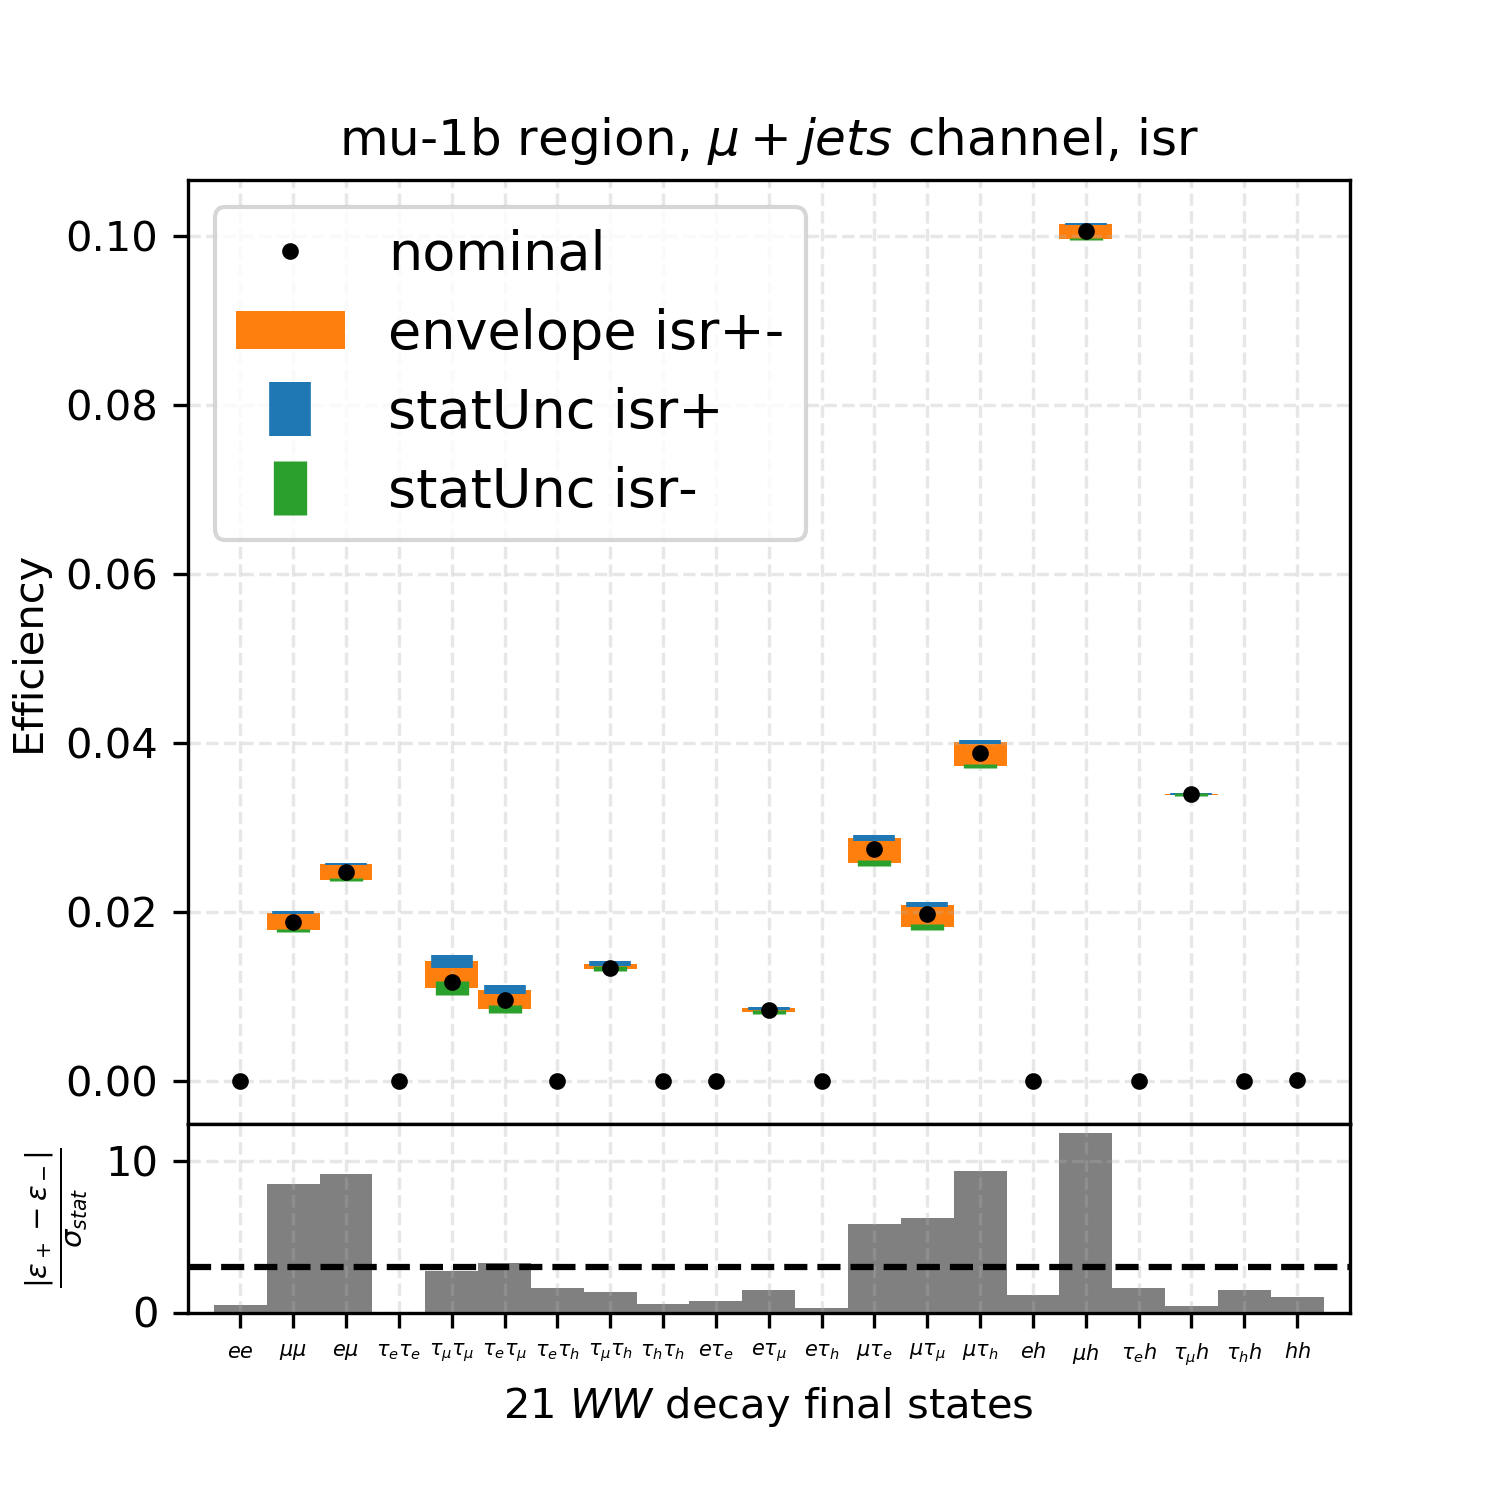
\includegraphics[width=0.24\textwidth]{chapters/Appendix/sectionTTSyst/figures/afterCorr/icata0_ch3_isr.png}

    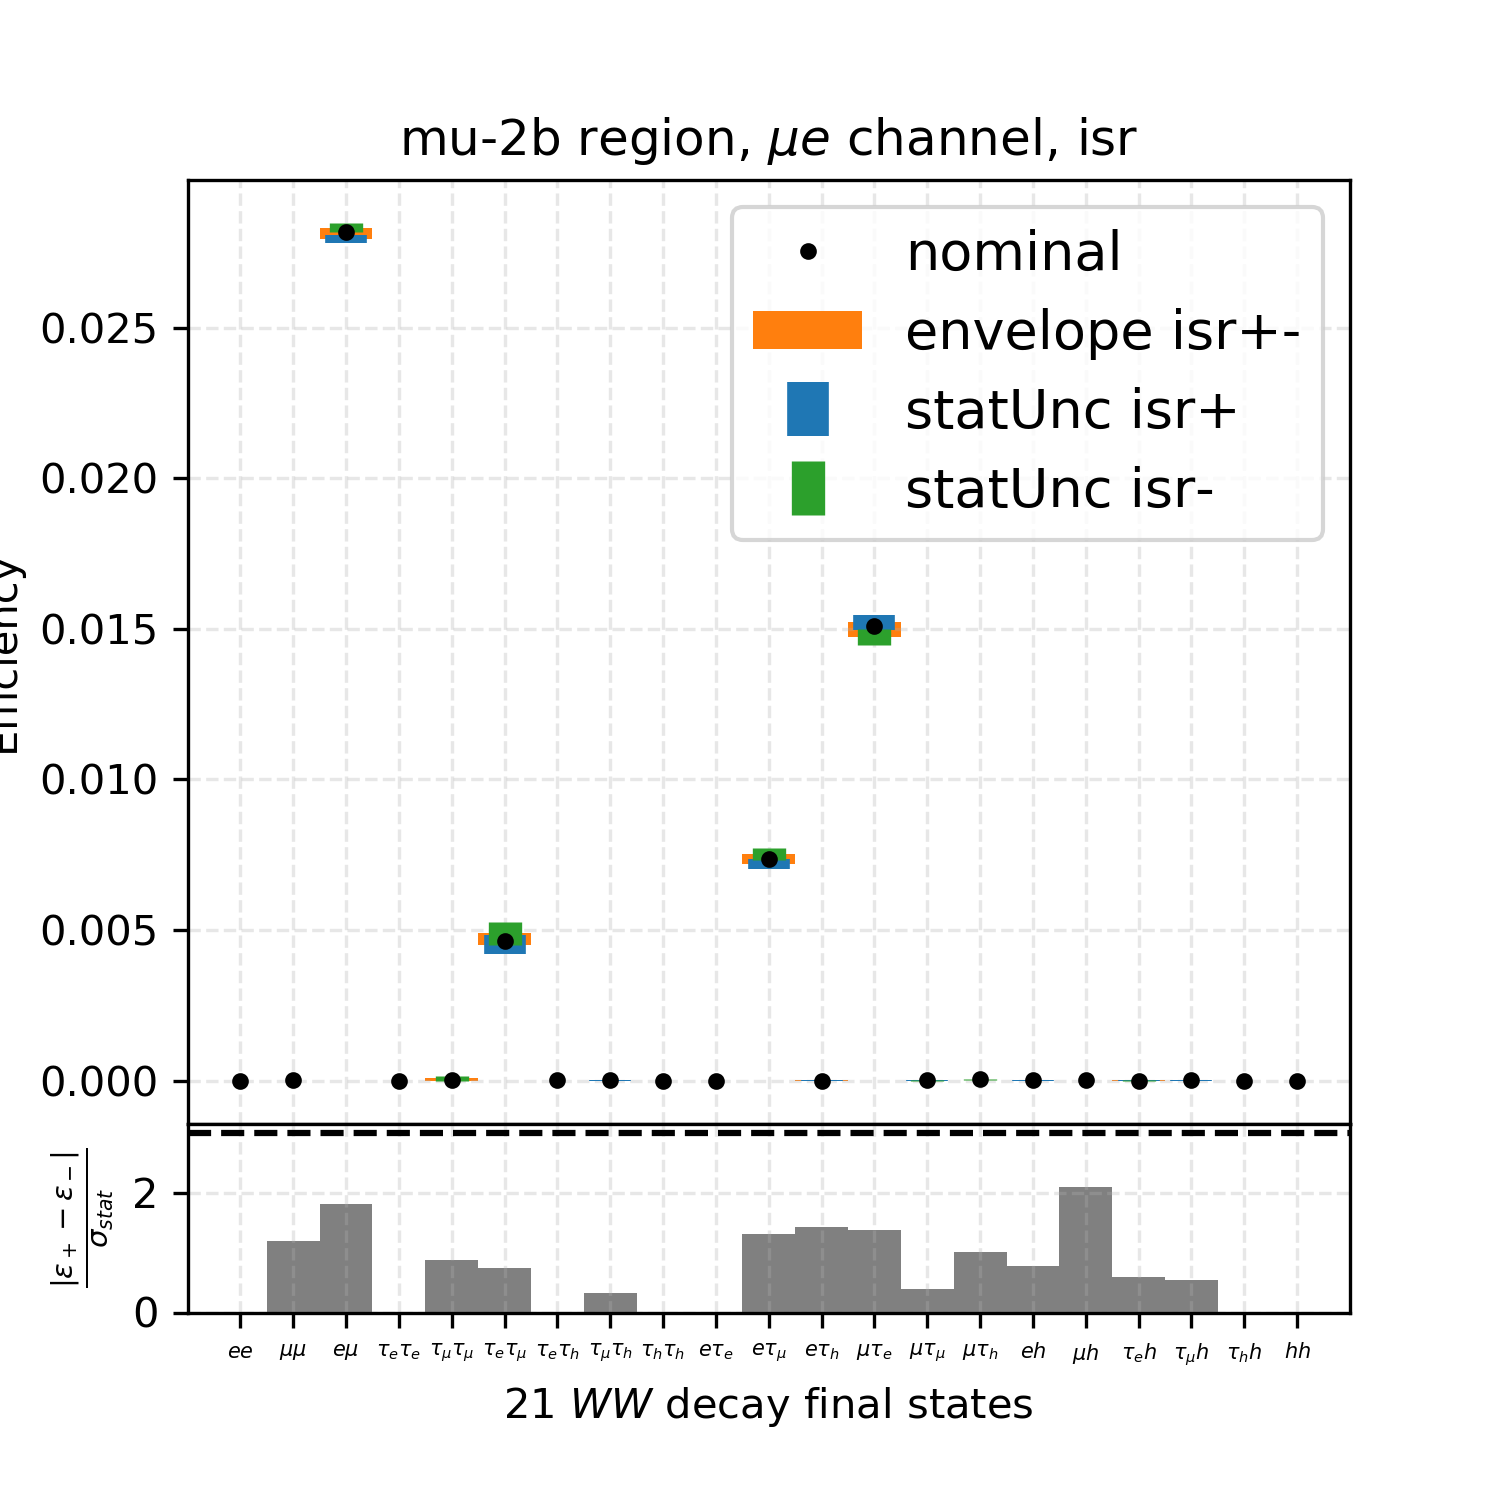
\includegraphics[width=0.24\textwidth]{chapters/Appendix/sectionTTSyst/figures/afterCorr/icata1_ch0_isr.png}
    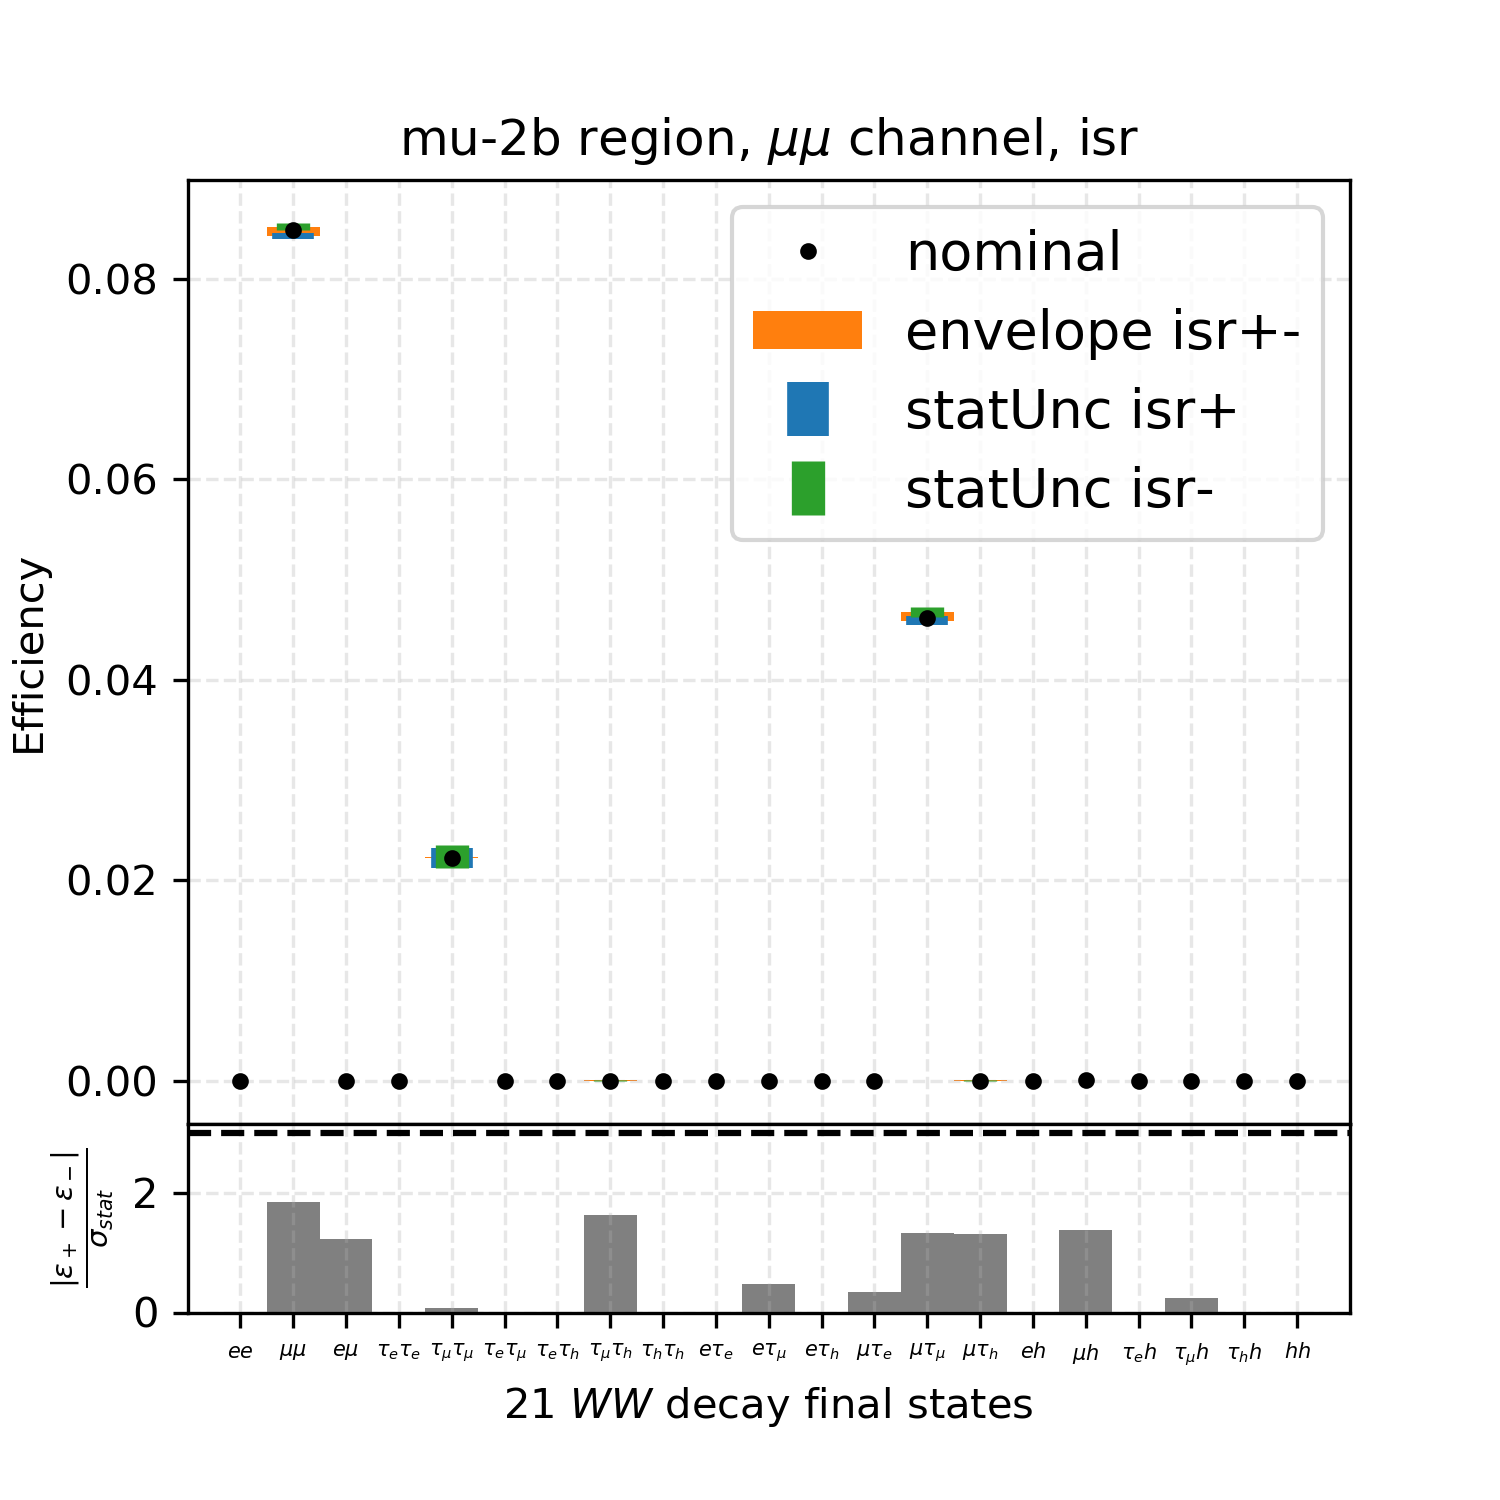
\includegraphics[width=0.24\textwidth]{chapters/Appendix/sectionTTSyst/figures/afterCorr/icata1_ch1_isr.png}
    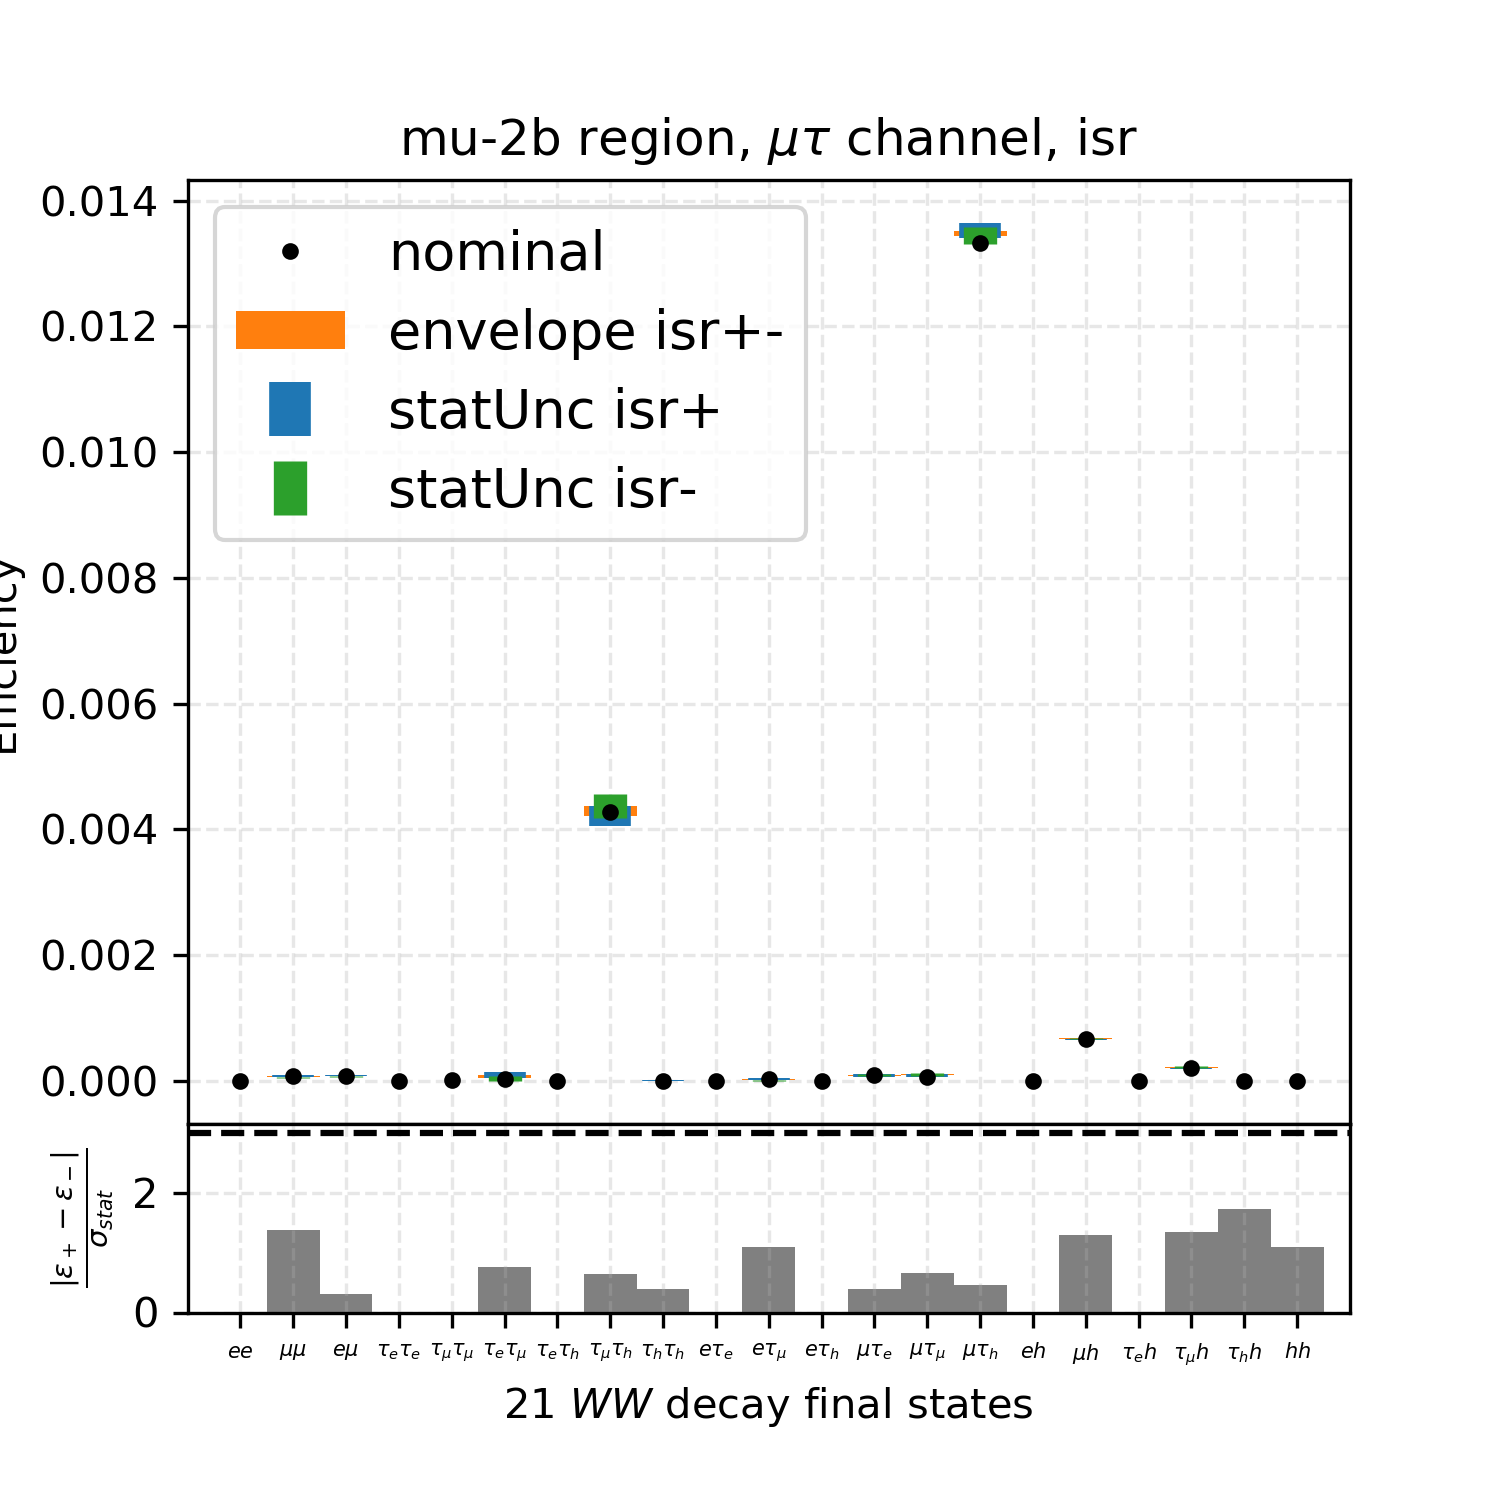
\includegraphics[width=0.24\textwidth]{chapters/Appendix/sectionTTSyst/figures/afterCorr/icata1_ch2_isr.png}
    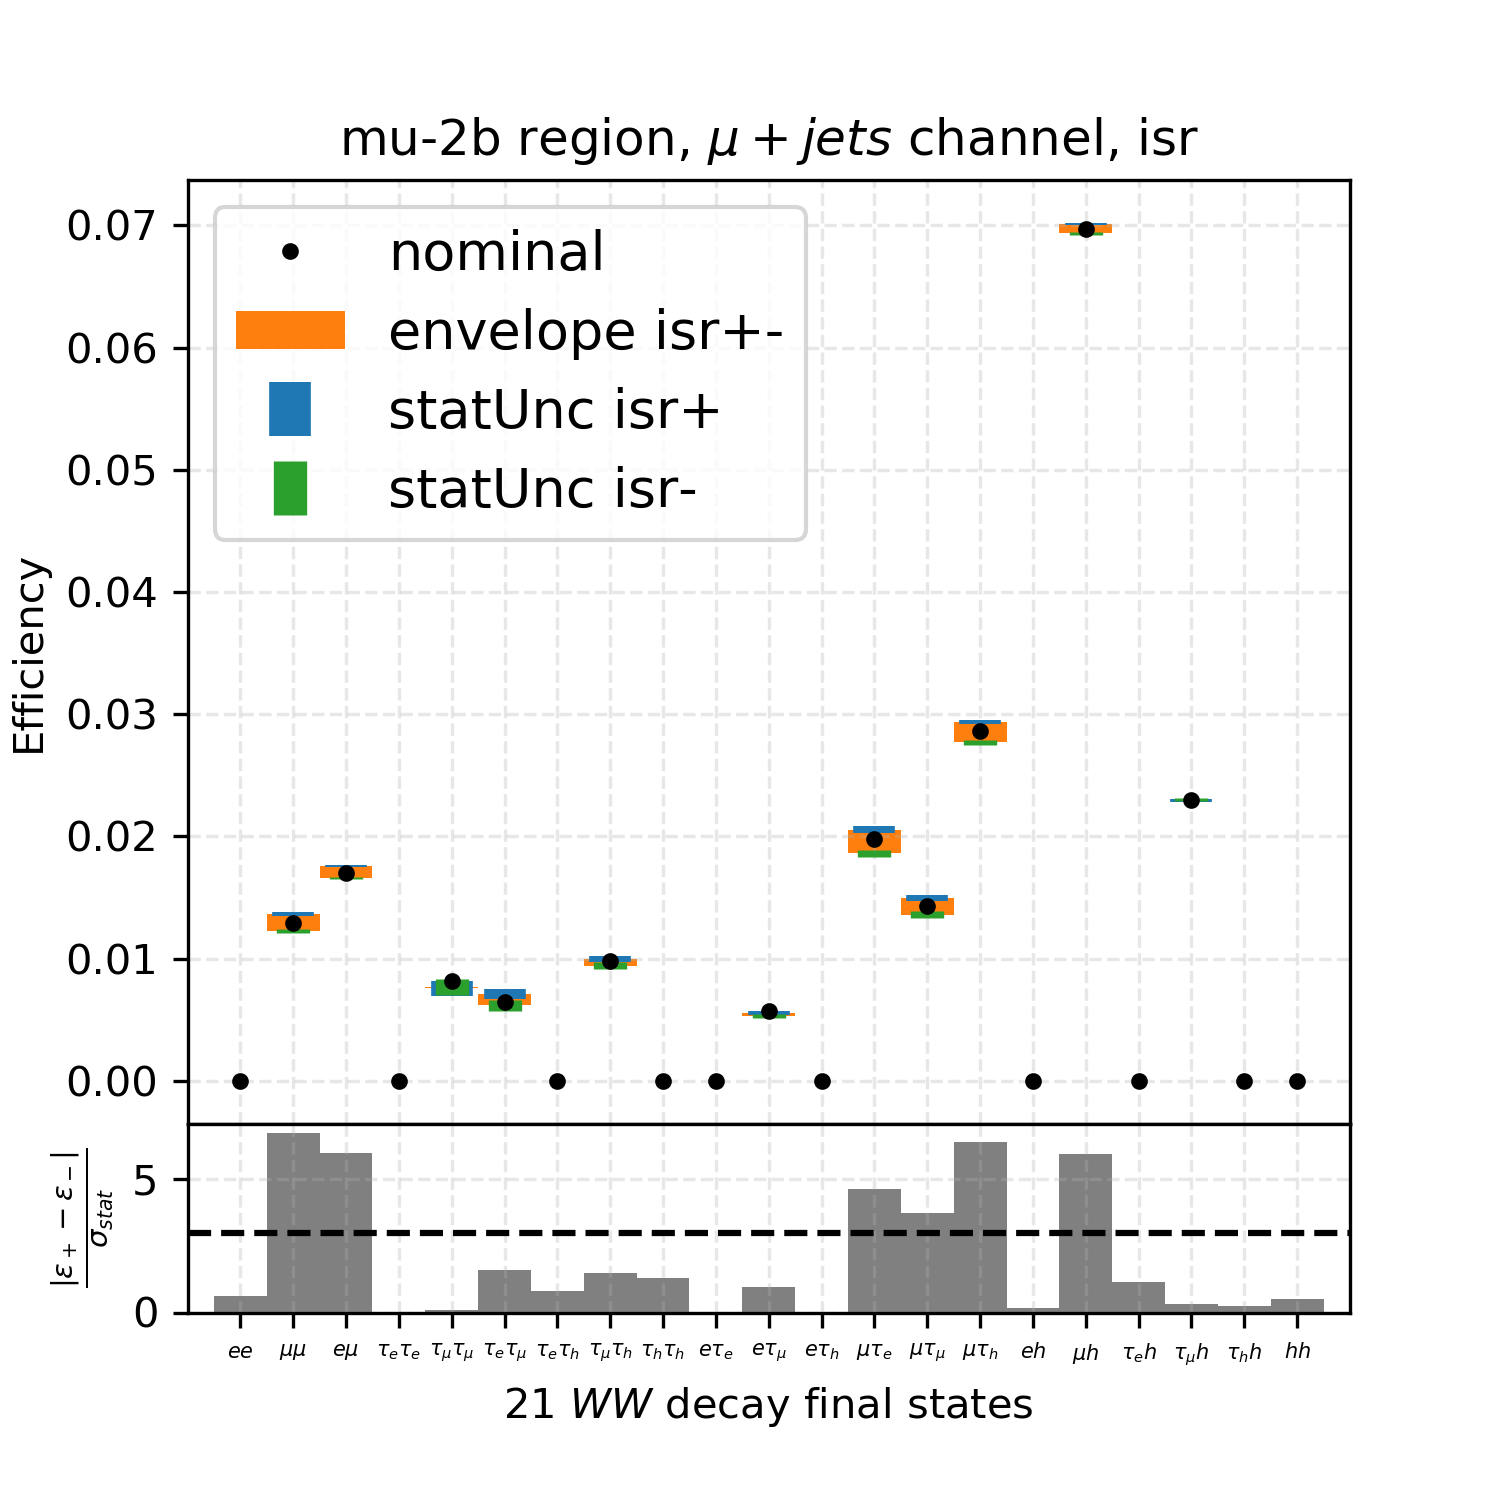
\includegraphics[width=0.24\textwidth]{chapters/Appendix/sectionTTSyst/figures/afterCorr/icata1_ch3_isr.png}
    
    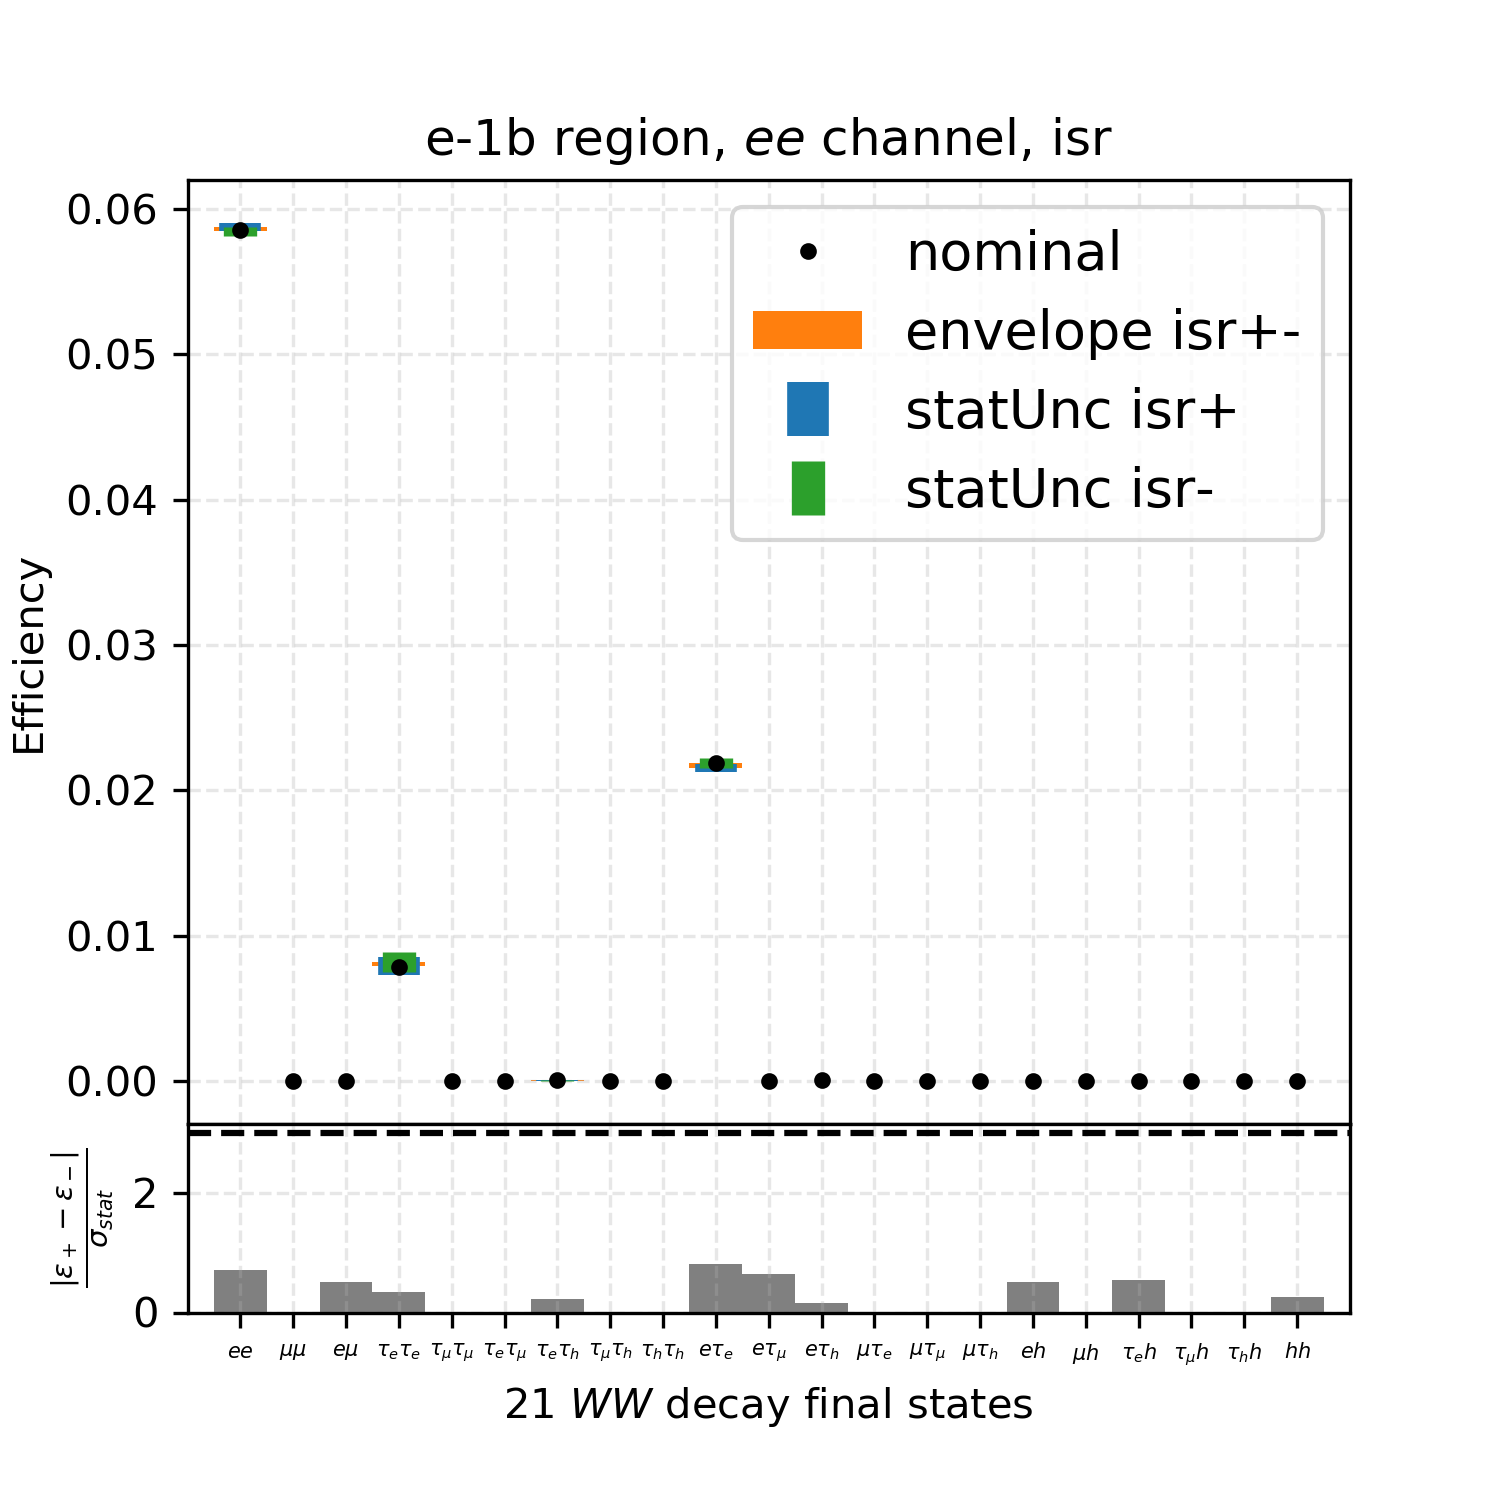
\includegraphics[width=0.24\textwidth]{chapters/Appendix/sectionTTSyst/figures/afterCorr/icata2_ch0_isr.png}
    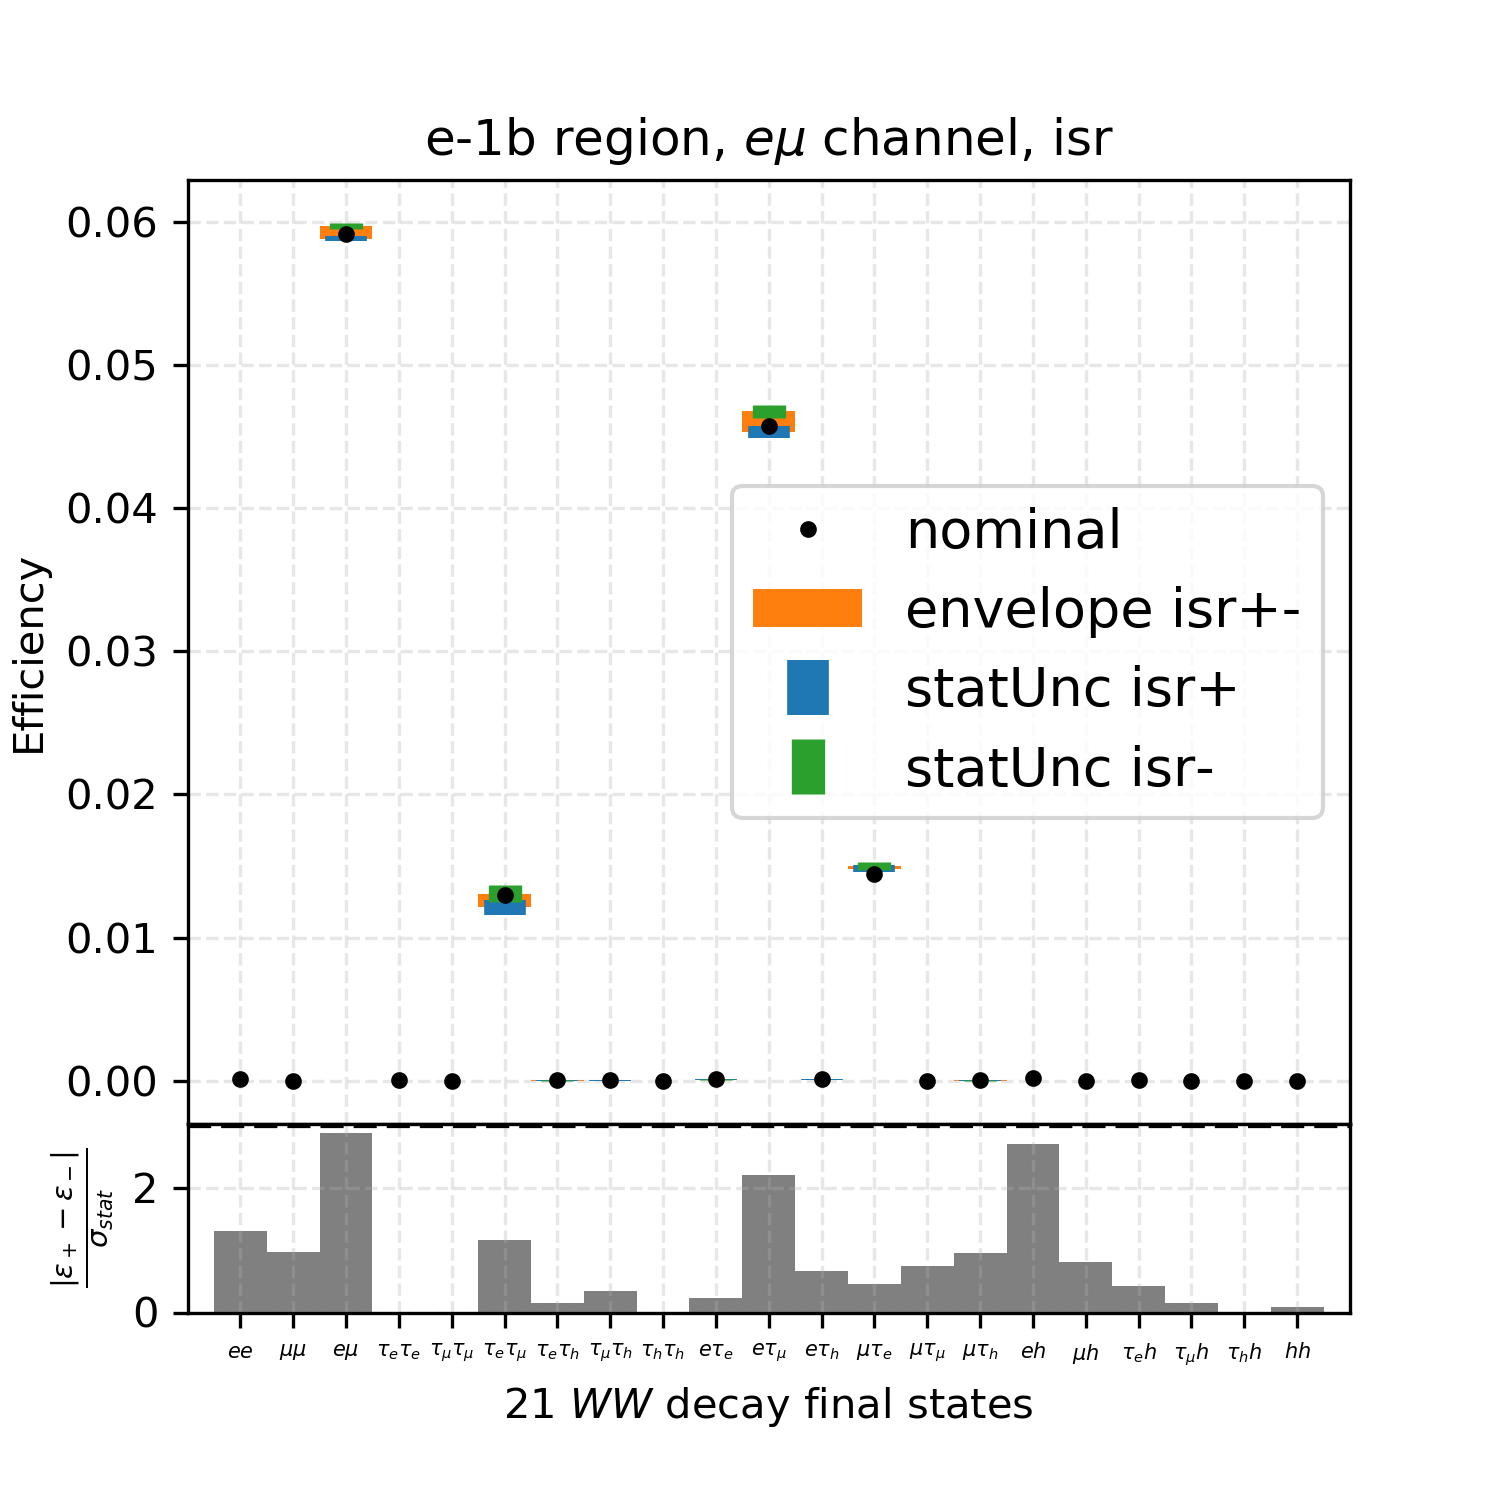
\includegraphics[width=0.24\textwidth]{chapters/Appendix/sectionTTSyst/figures/afterCorr/icata2_ch1_isr.png}
    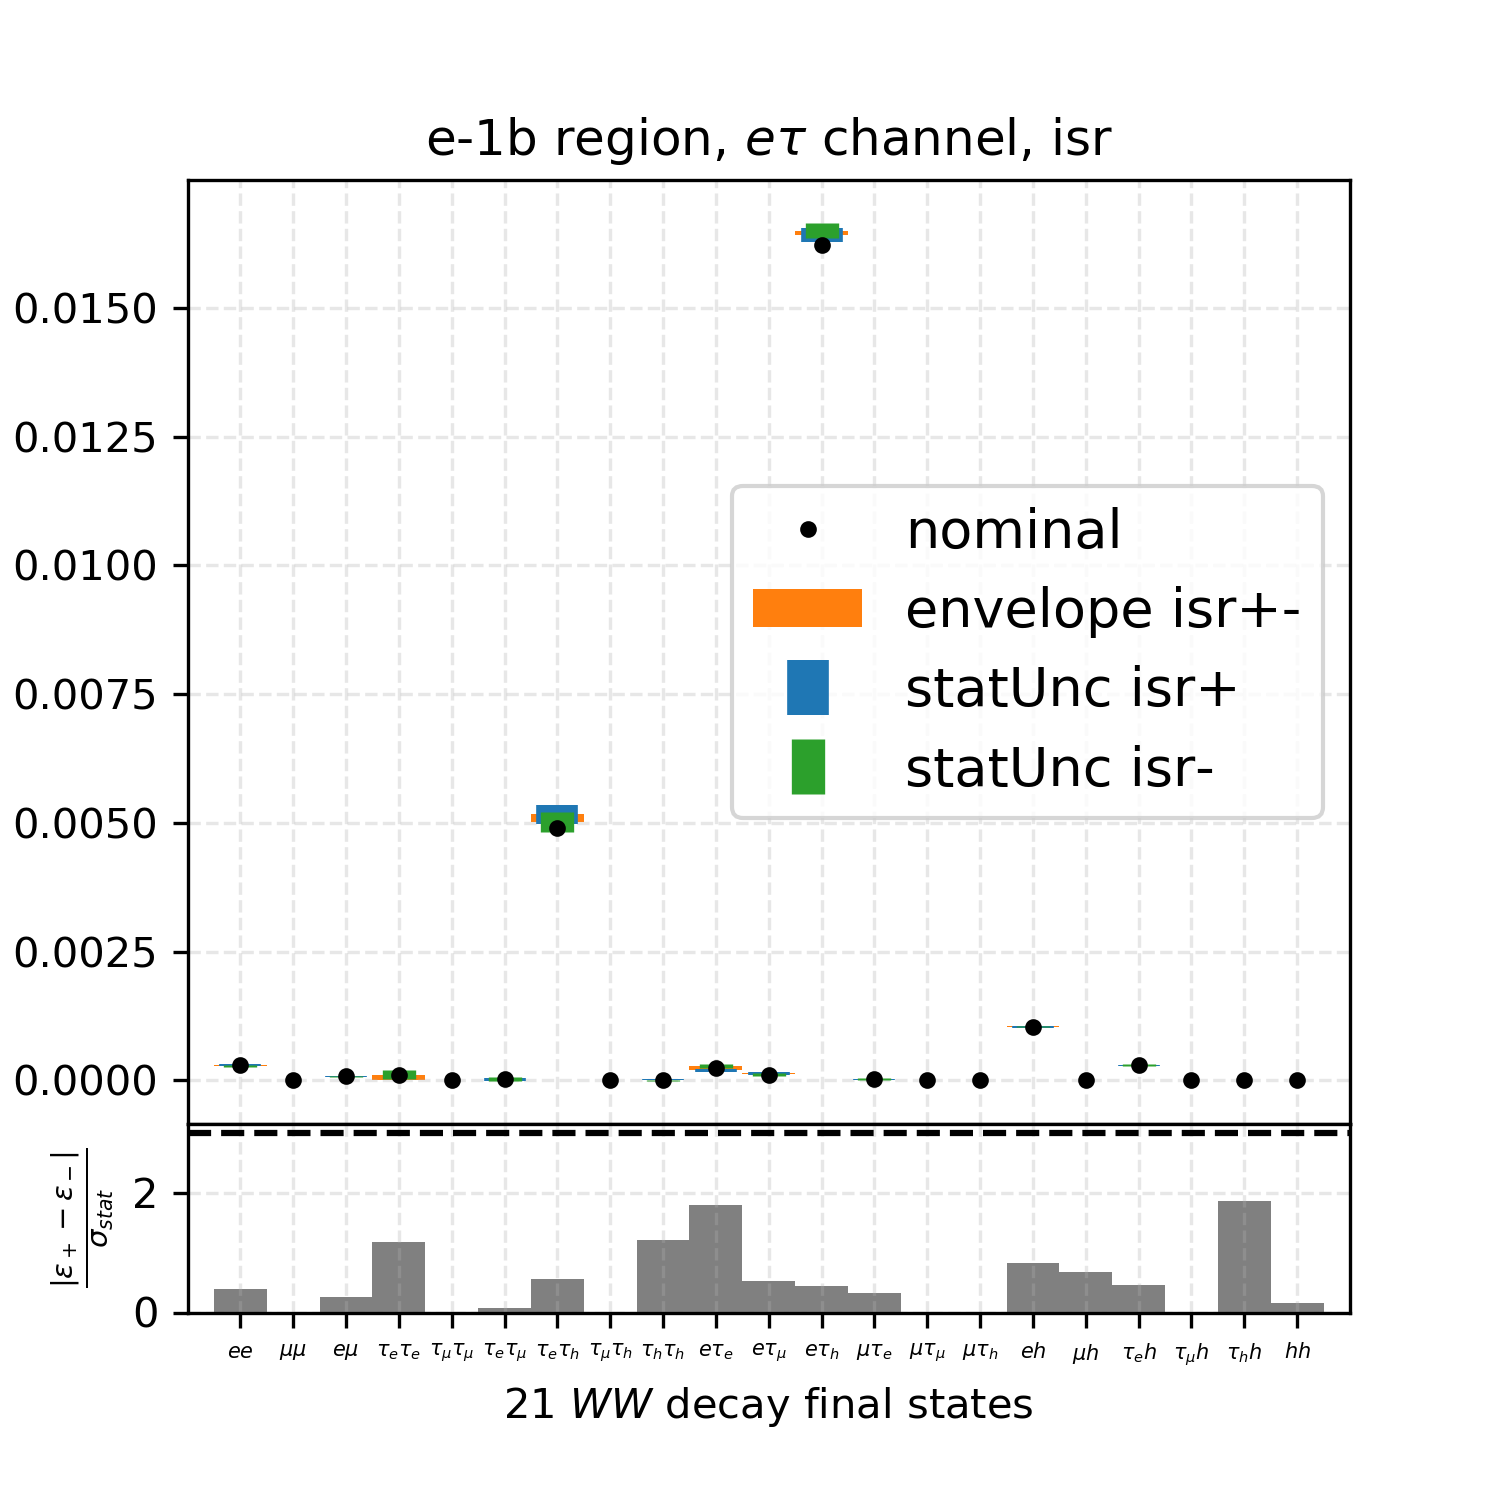
\includegraphics[width=0.24\textwidth]{chapters/Appendix/sectionTTSyst/figures/afterCorr/icata2_ch2_isr.png}
    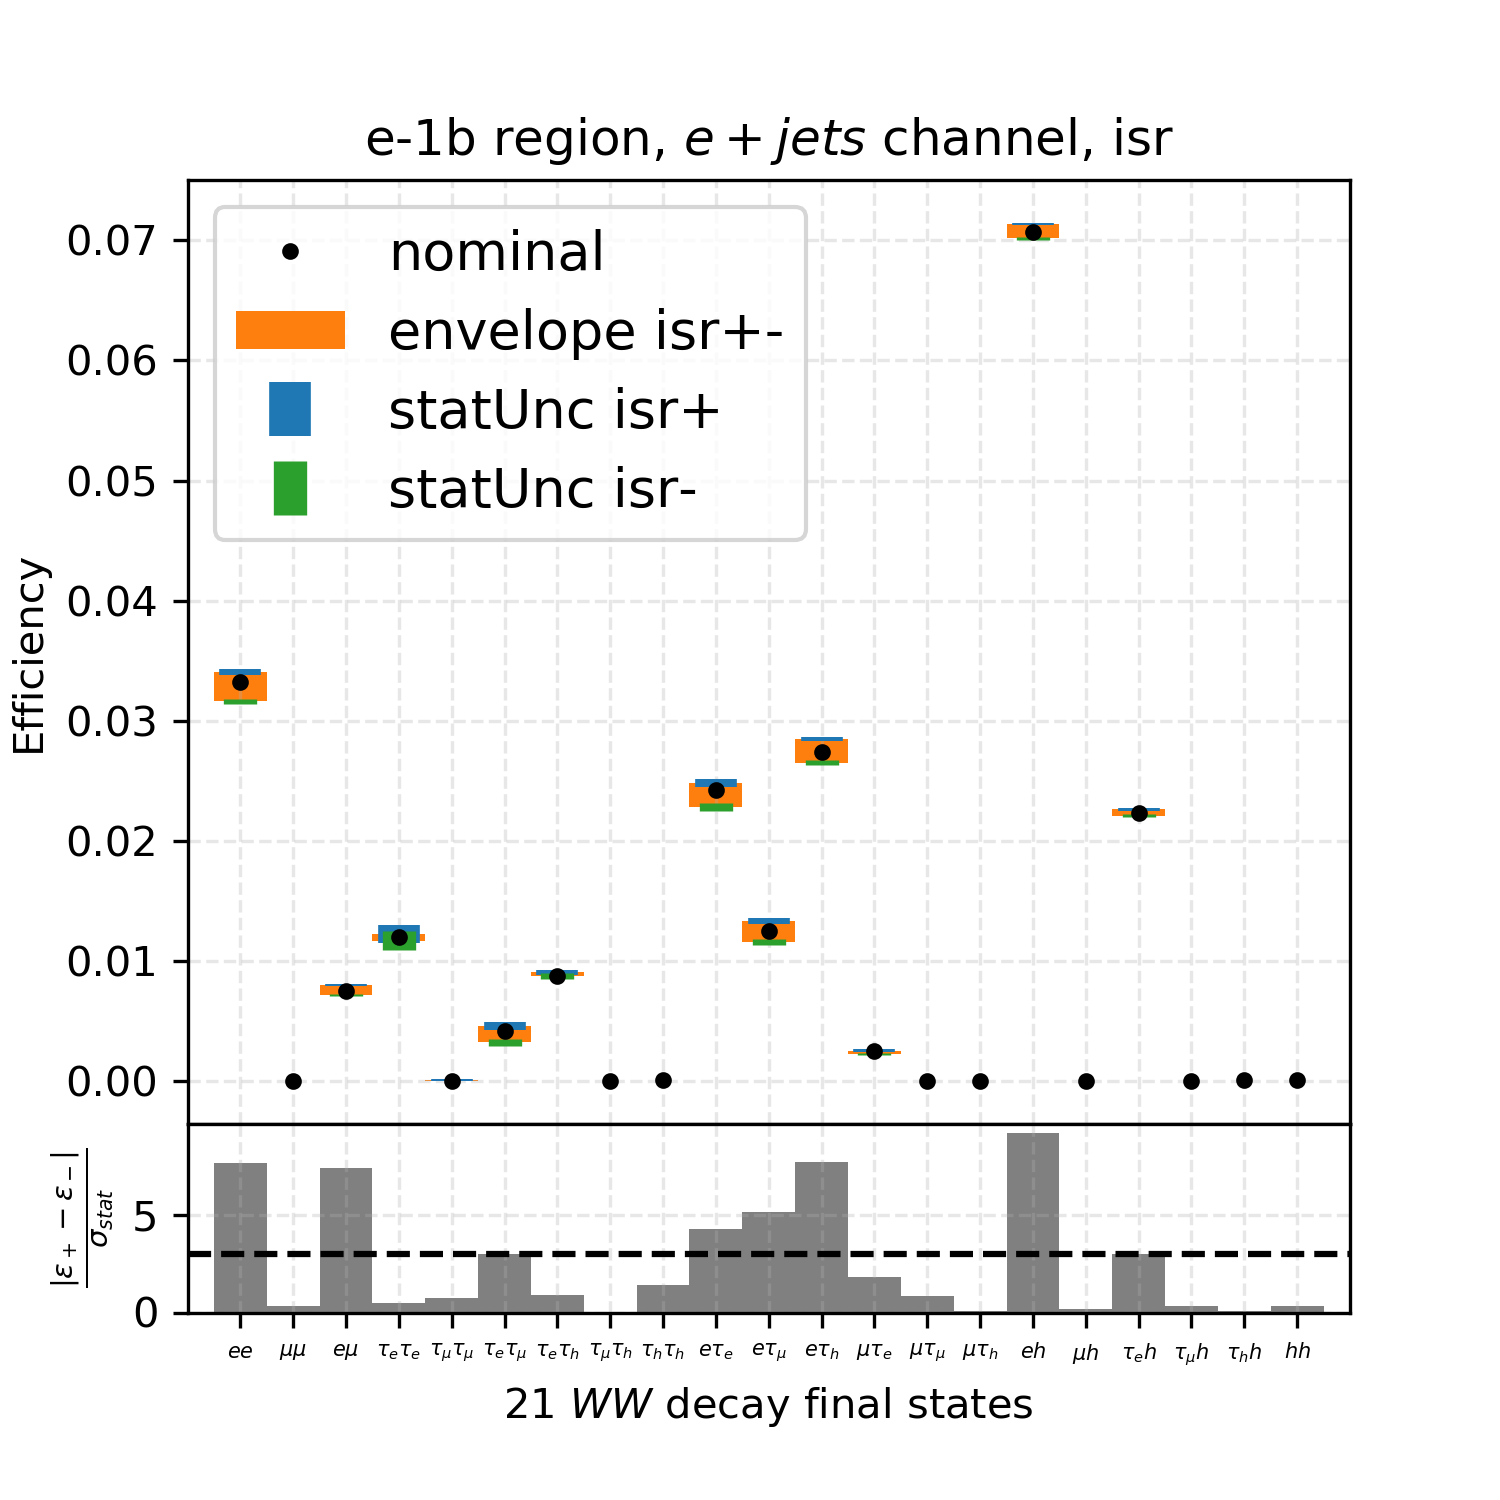
\includegraphics[width=0.24\textwidth]{chapters/Appendix/sectionTTSyst/figures/afterCorr/icata2_ch3_isr.png}

    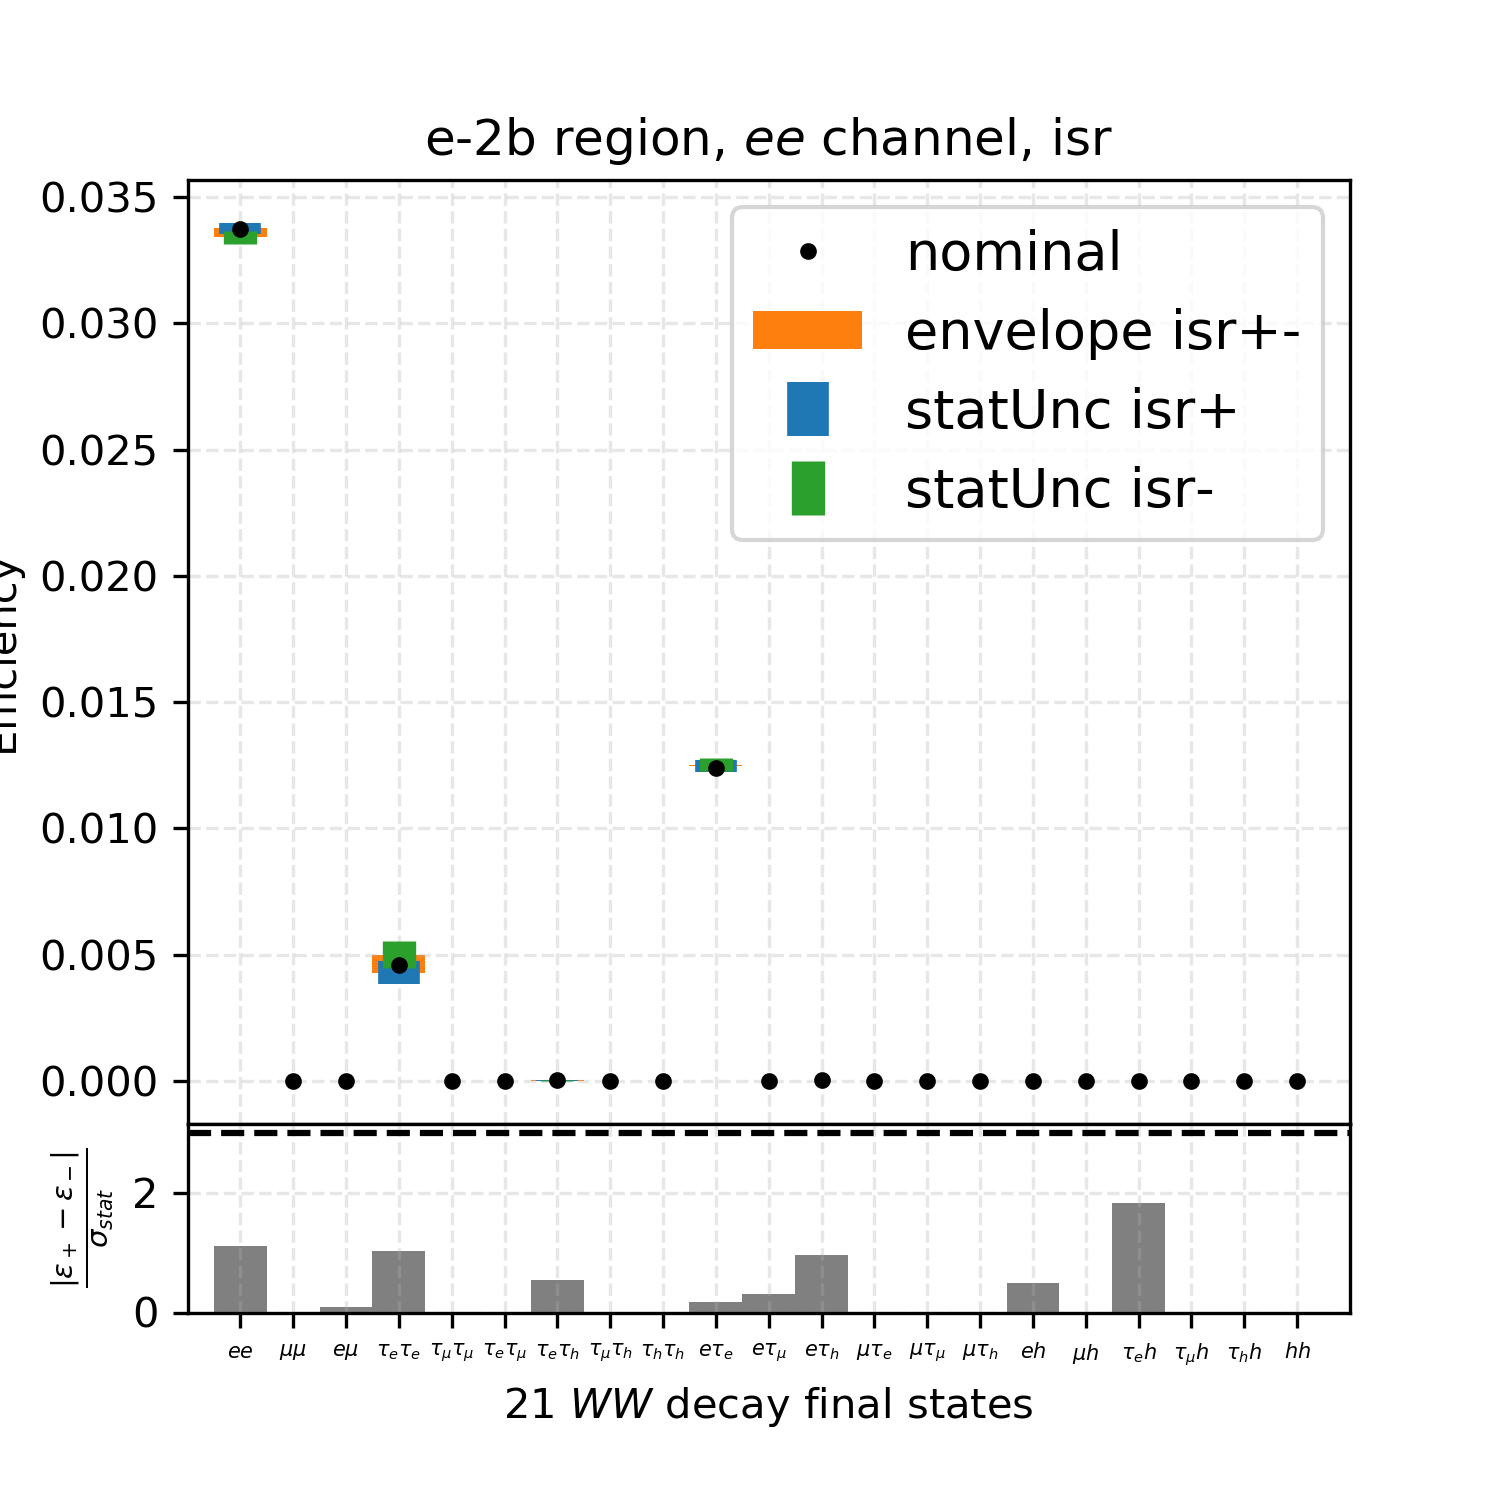
\includegraphics[width=0.24\textwidth]{chapters/Appendix/sectionTTSyst/figures/afterCorr/icata3_ch0_isr.png}
    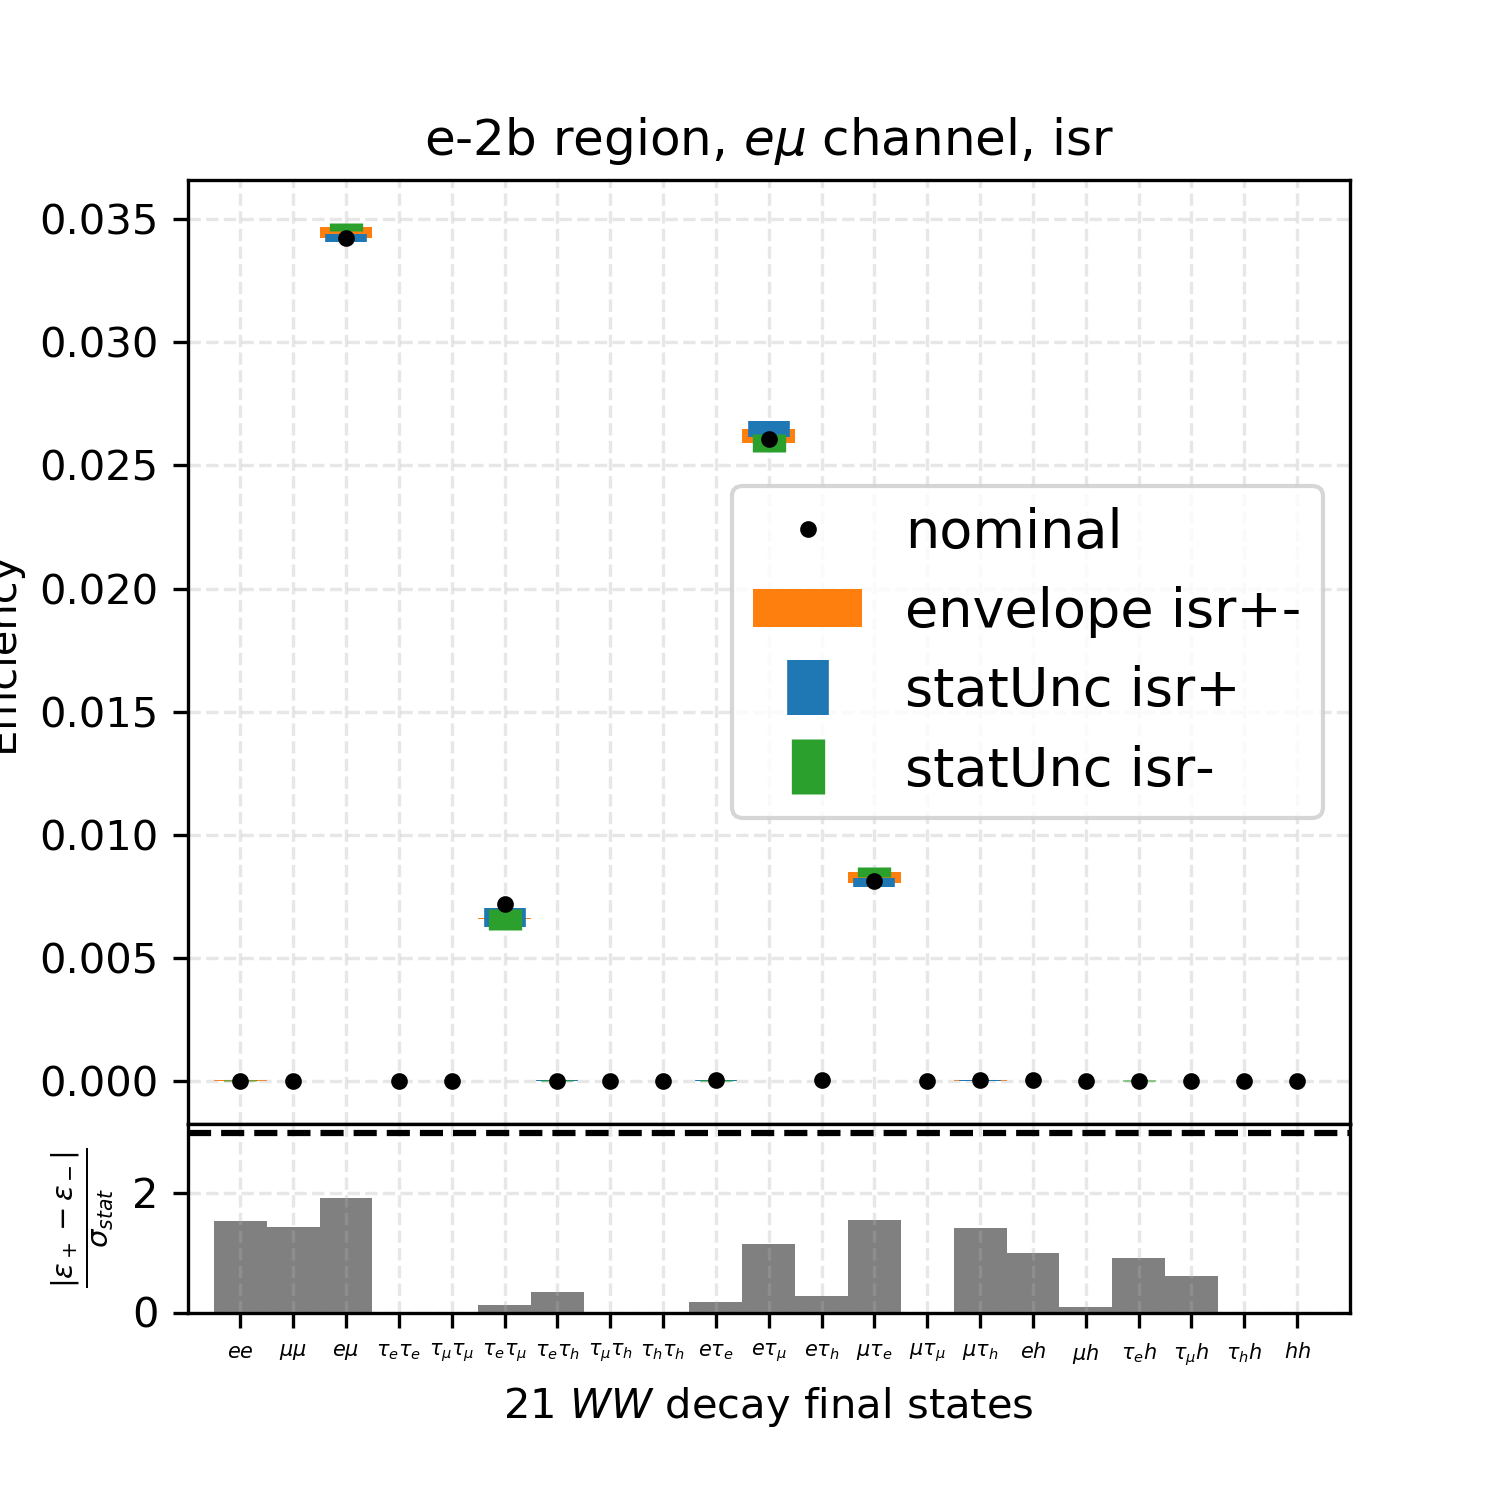
\includegraphics[width=0.24\textwidth]{chapters/Appendix/sectionTTSyst/figures/afterCorr/icata3_ch1_isr.png}
    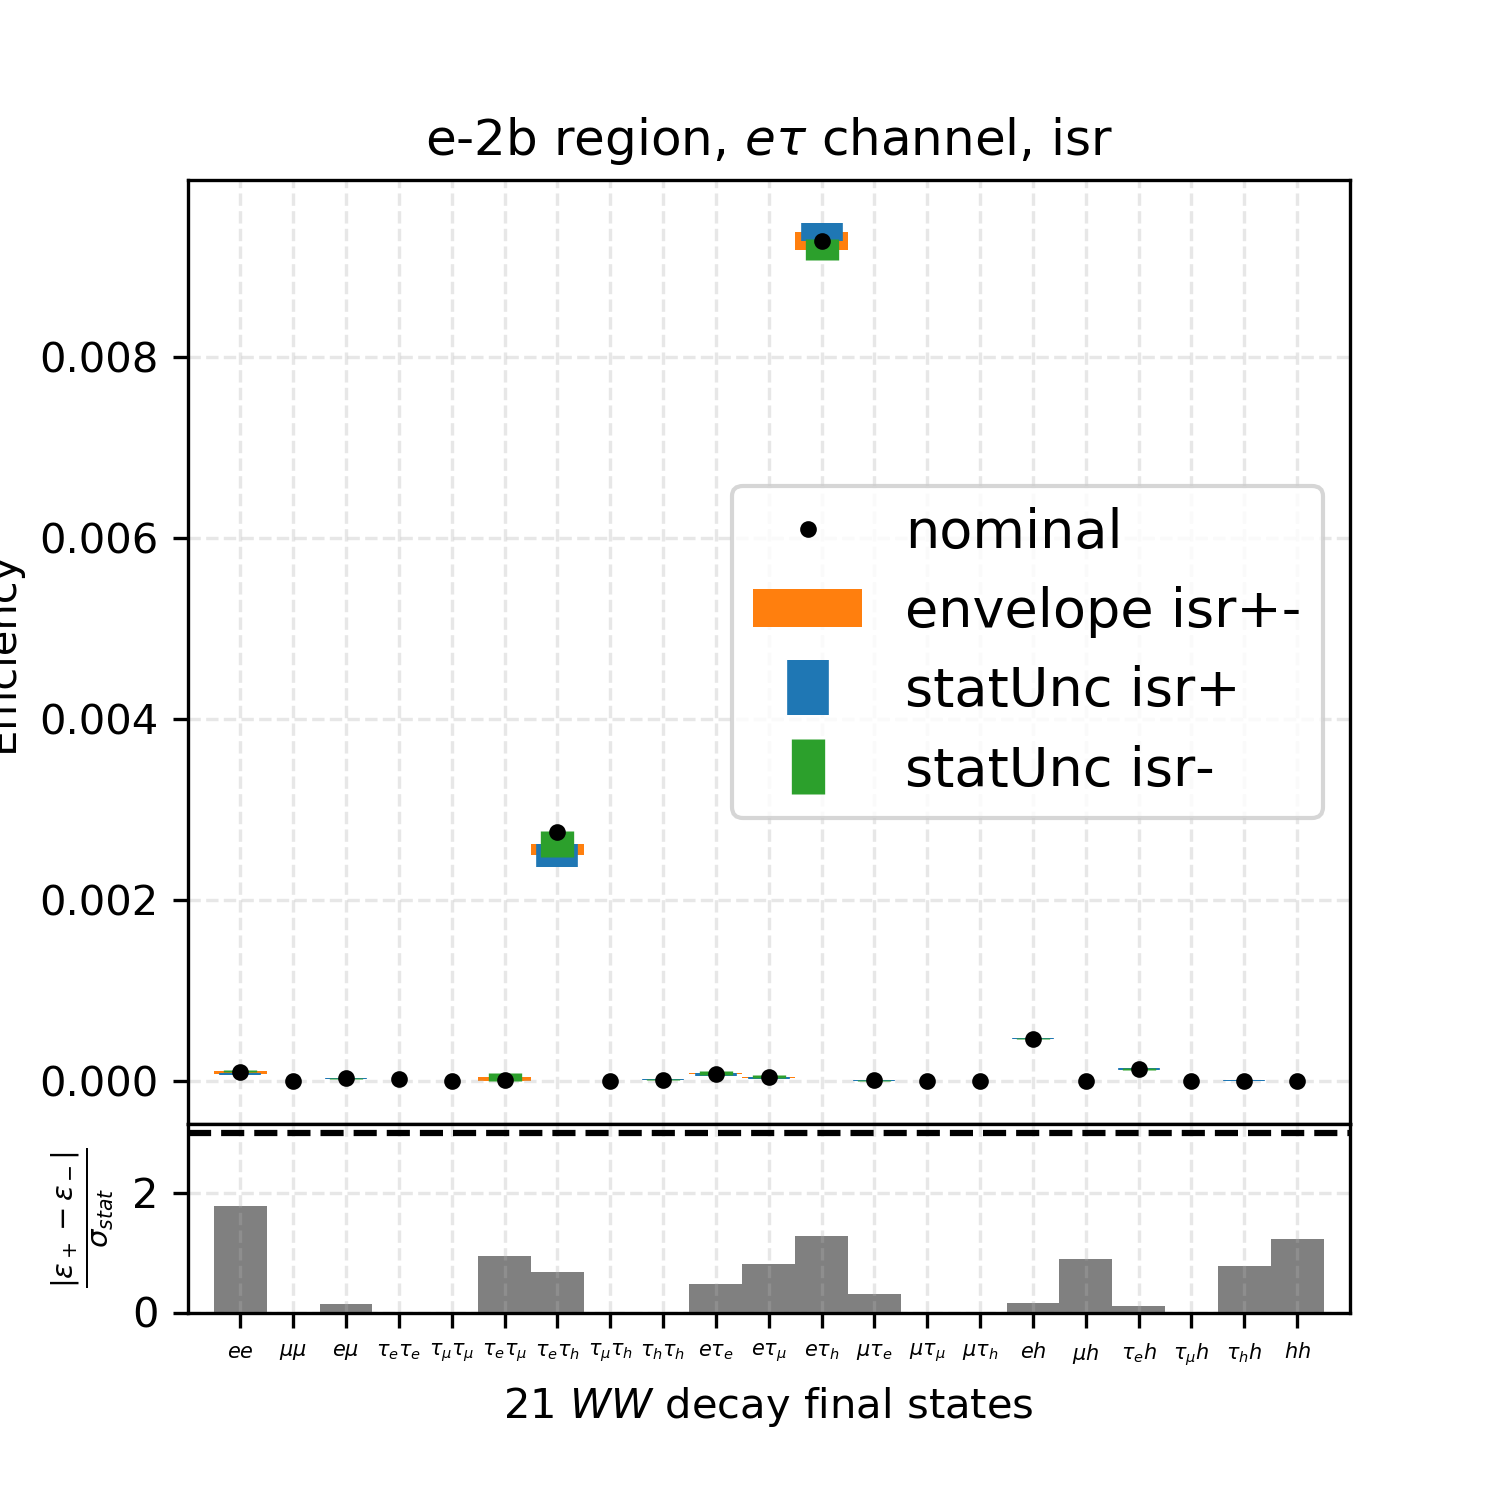
\includegraphics[width=0.24\textwidth]{chapters/Appendix/sectionTTSyst/figures/afterCorr/icata3_ch2_isr.png}
    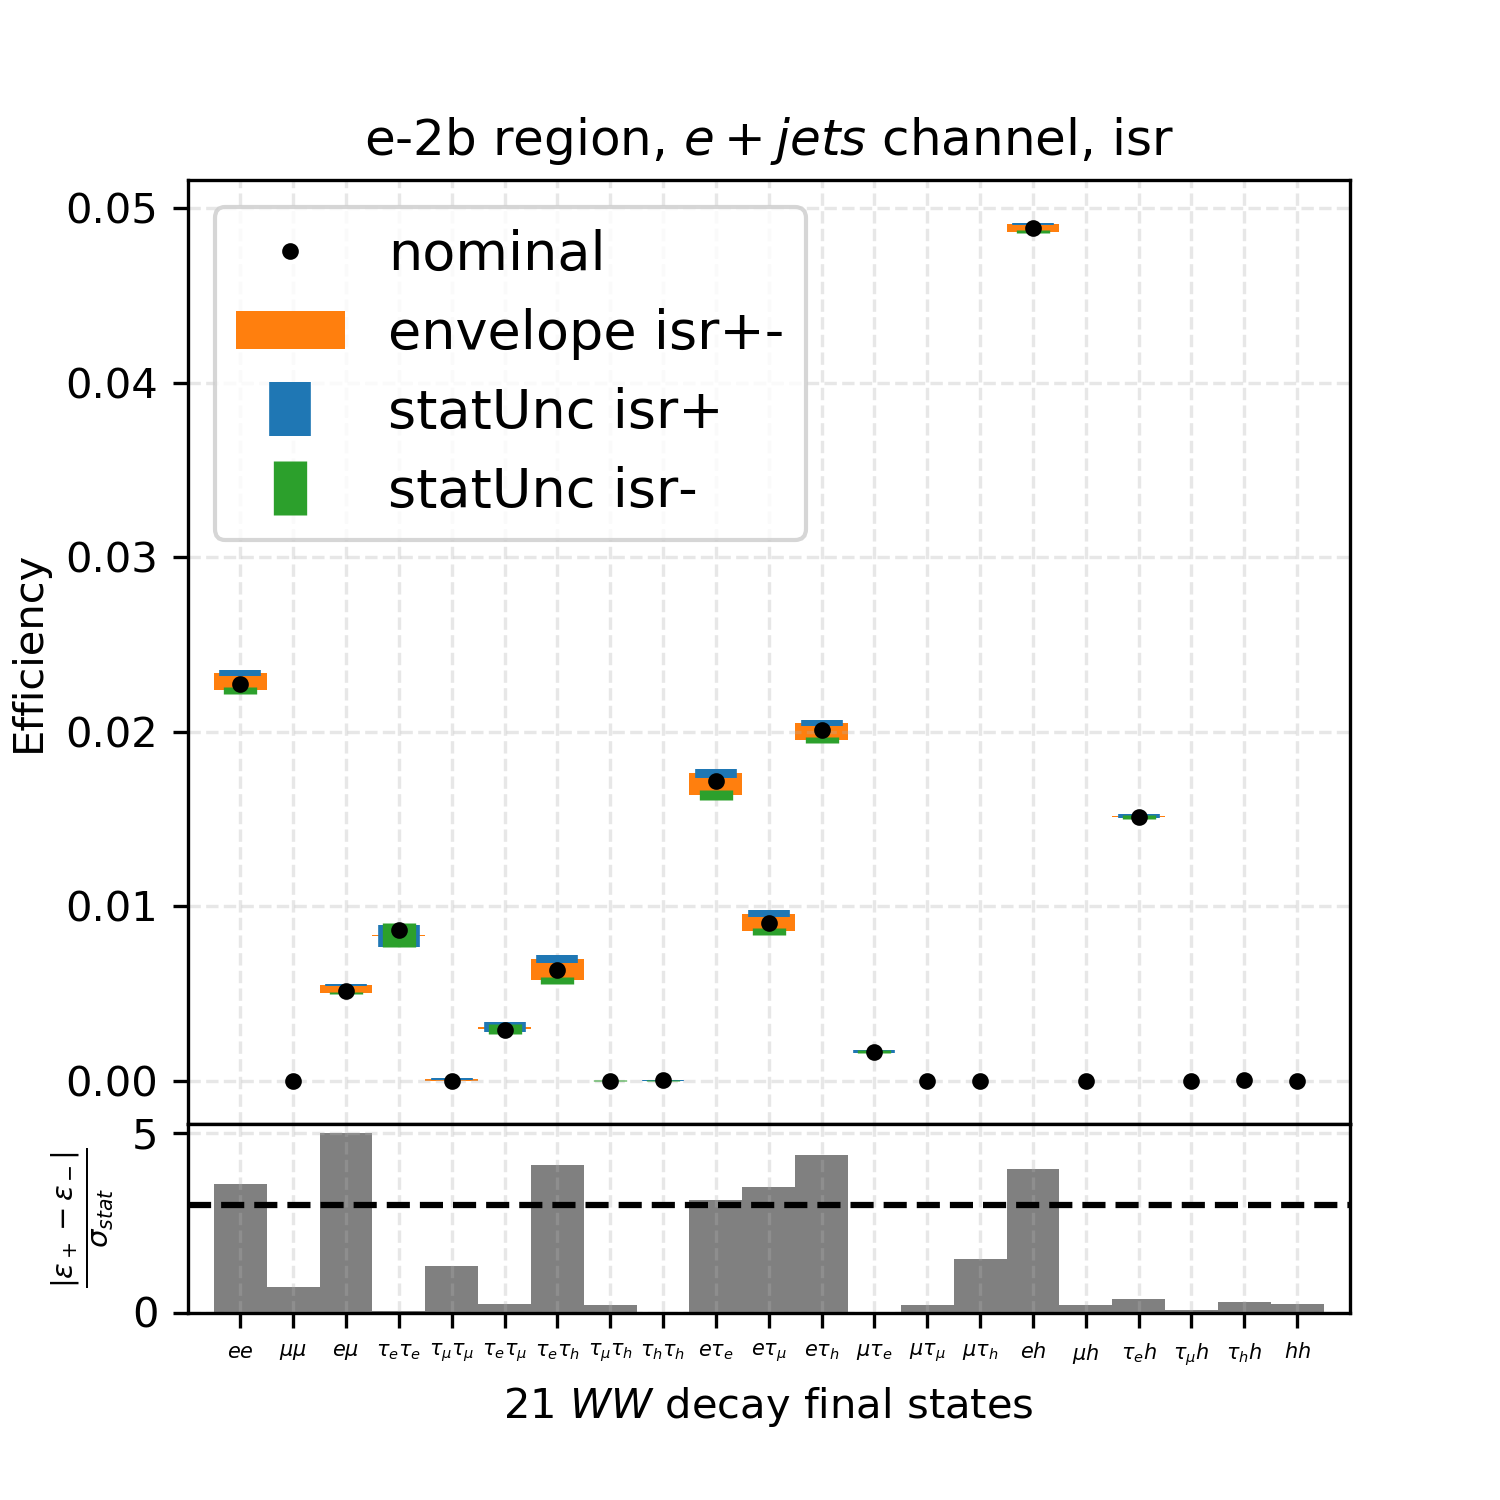
\includegraphics[width=0.24\textwidth]{chapters/Appendix/sectionTTSyst/figures/afterCorr/icata3_ch3_isr.png}
    
    \caption{ISR envelops on 21 efficiencies. VTight WP is shown.}
    \label{fig:appendix:reweighttt:effAfterCorrISR}
\end{figure}




\begin{figure}
    \centering
    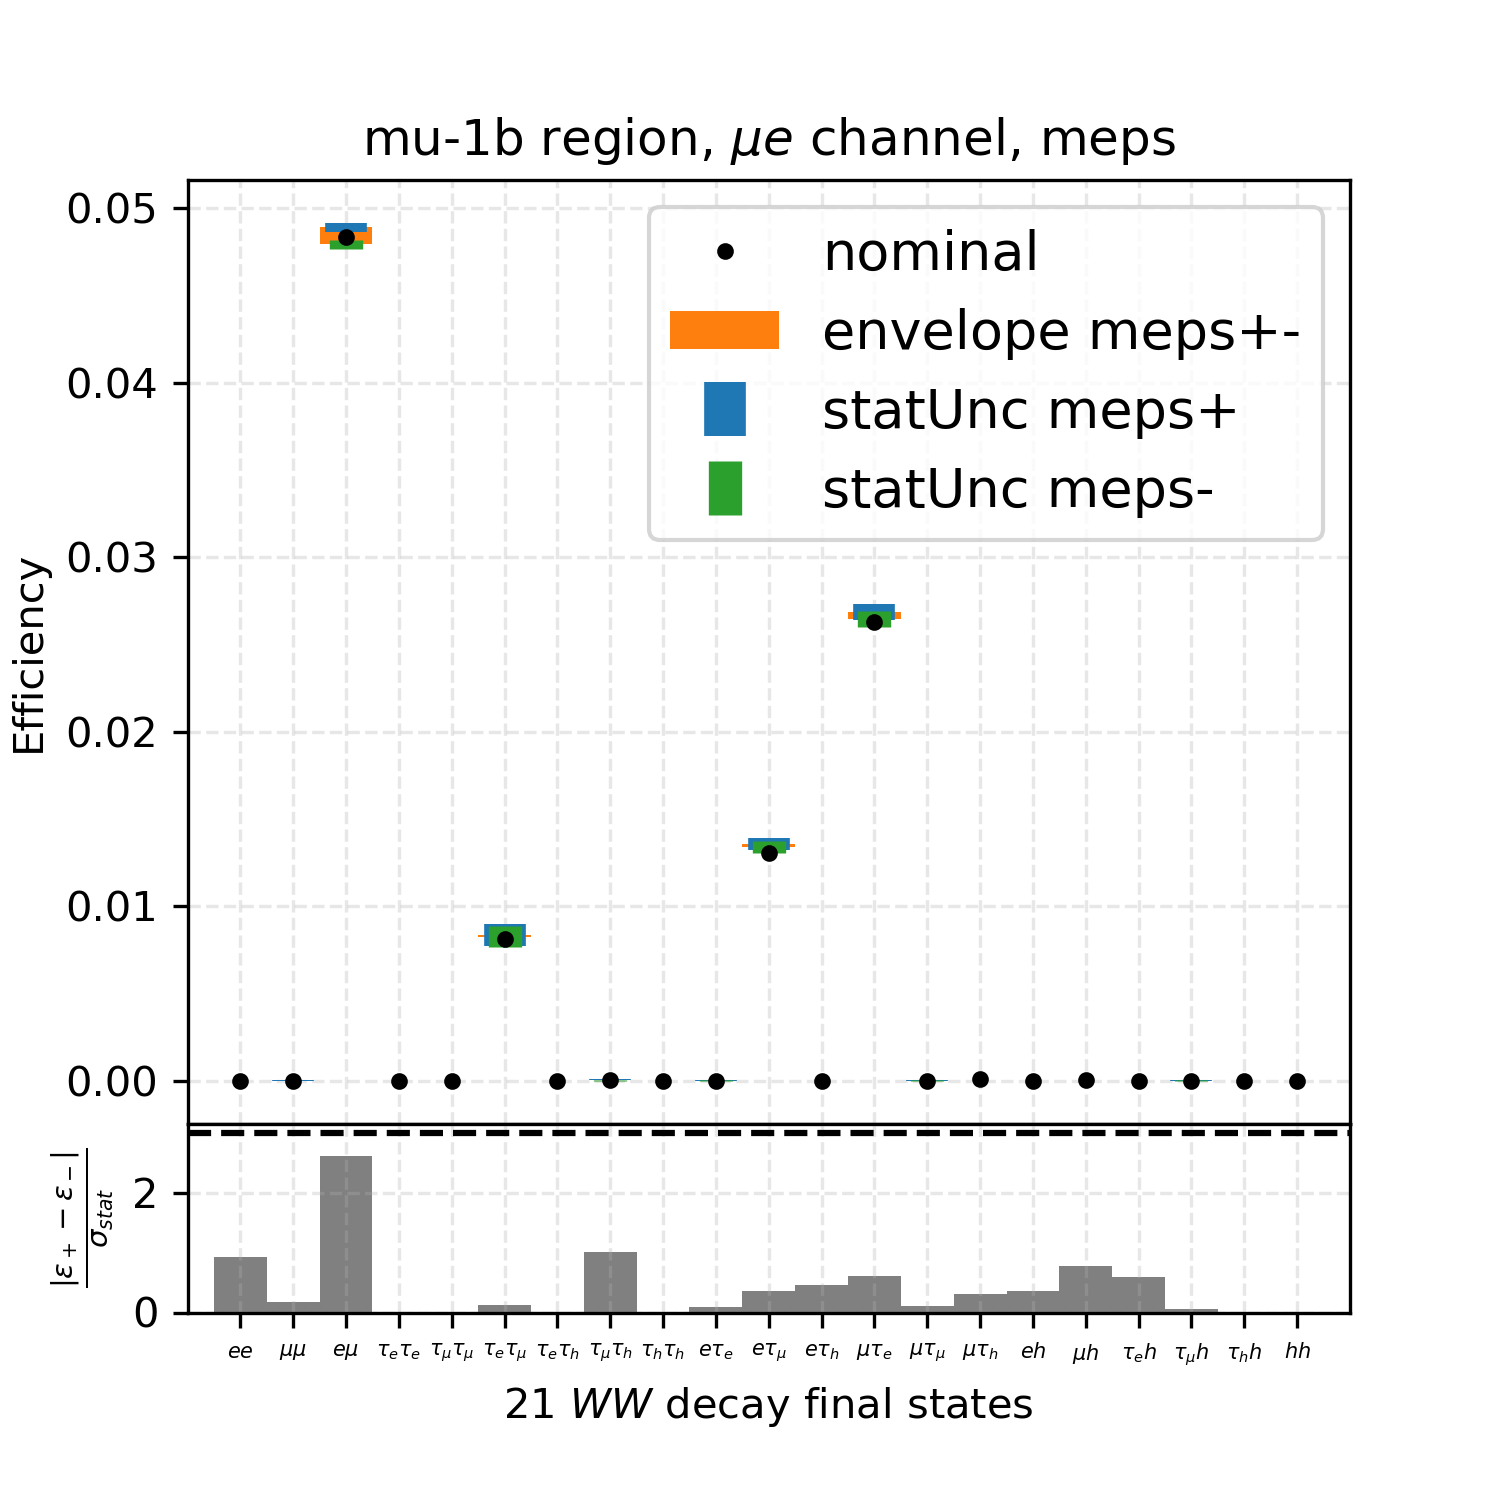
\includegraphics[width=0.24\textwidth]{chapters/Appendix/sectionTTSyst/figures/afterCorr/icata0_ch0_meps.png}
    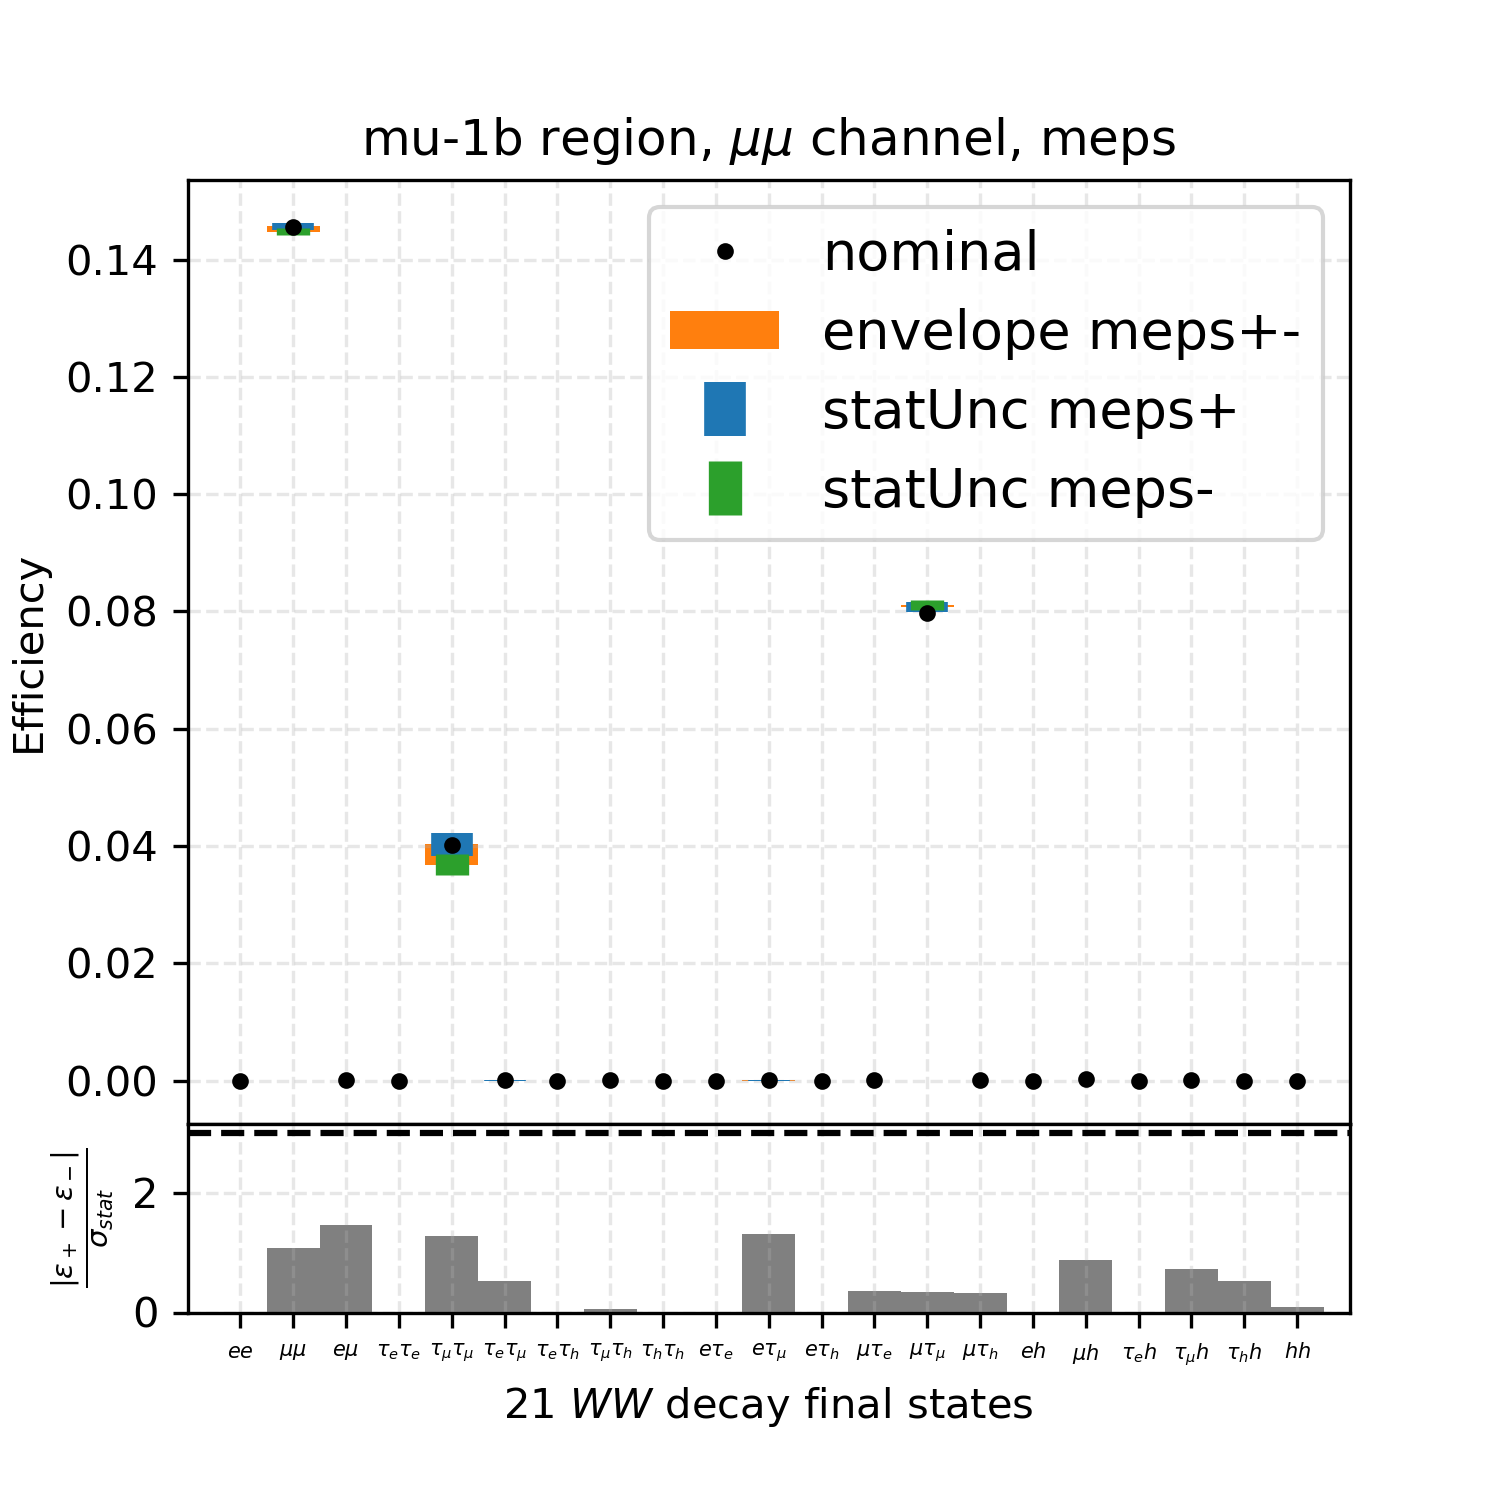
\includegraphics[width=0.24\textwidth]{chapters/Appendix/sectionTTSyst/figures/afterCorr/icata0_ch1_meps.png}
    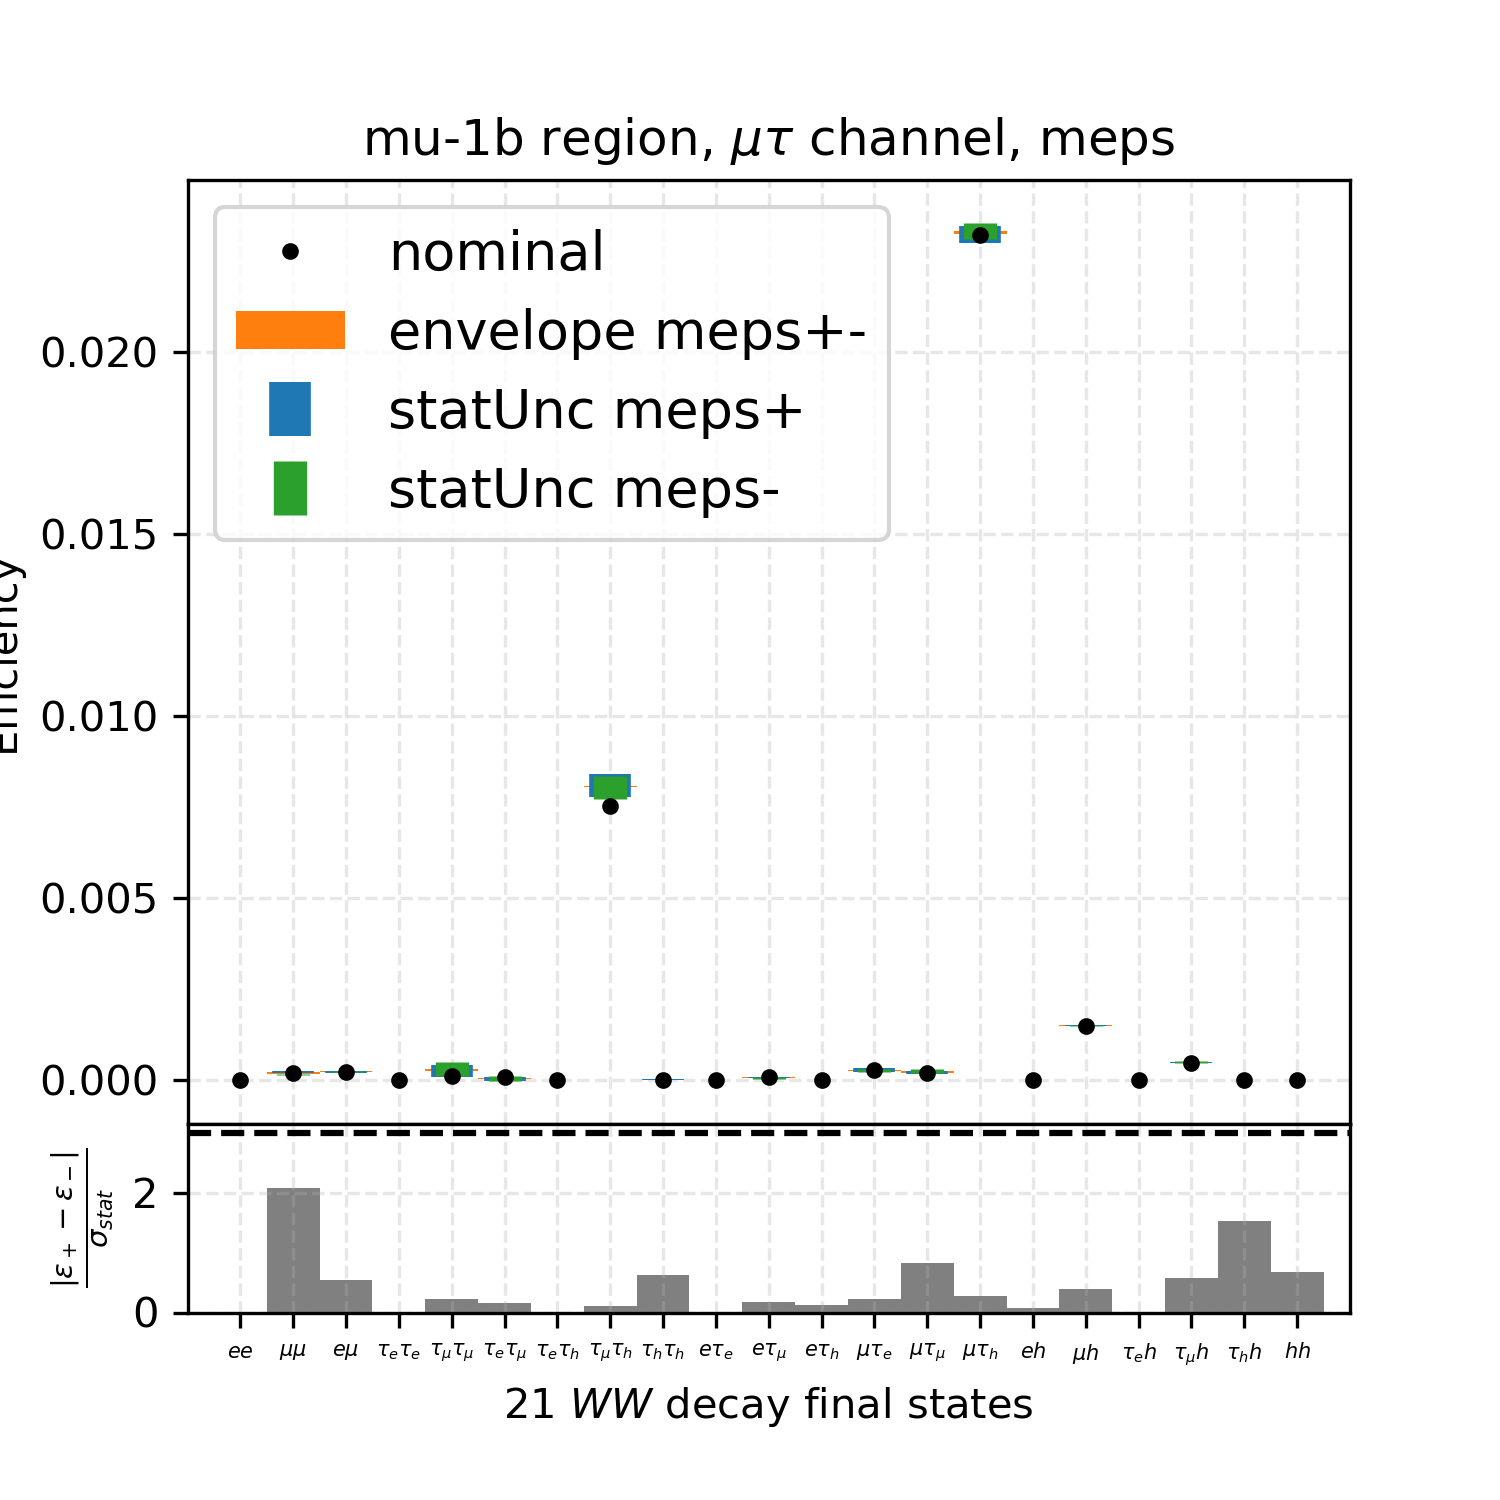
\includegraphics[width=0.24\textwidth]{chapters/Appendix/sectionTTSyst/figures/afterCorr/icata0_ch2_meps.png}
    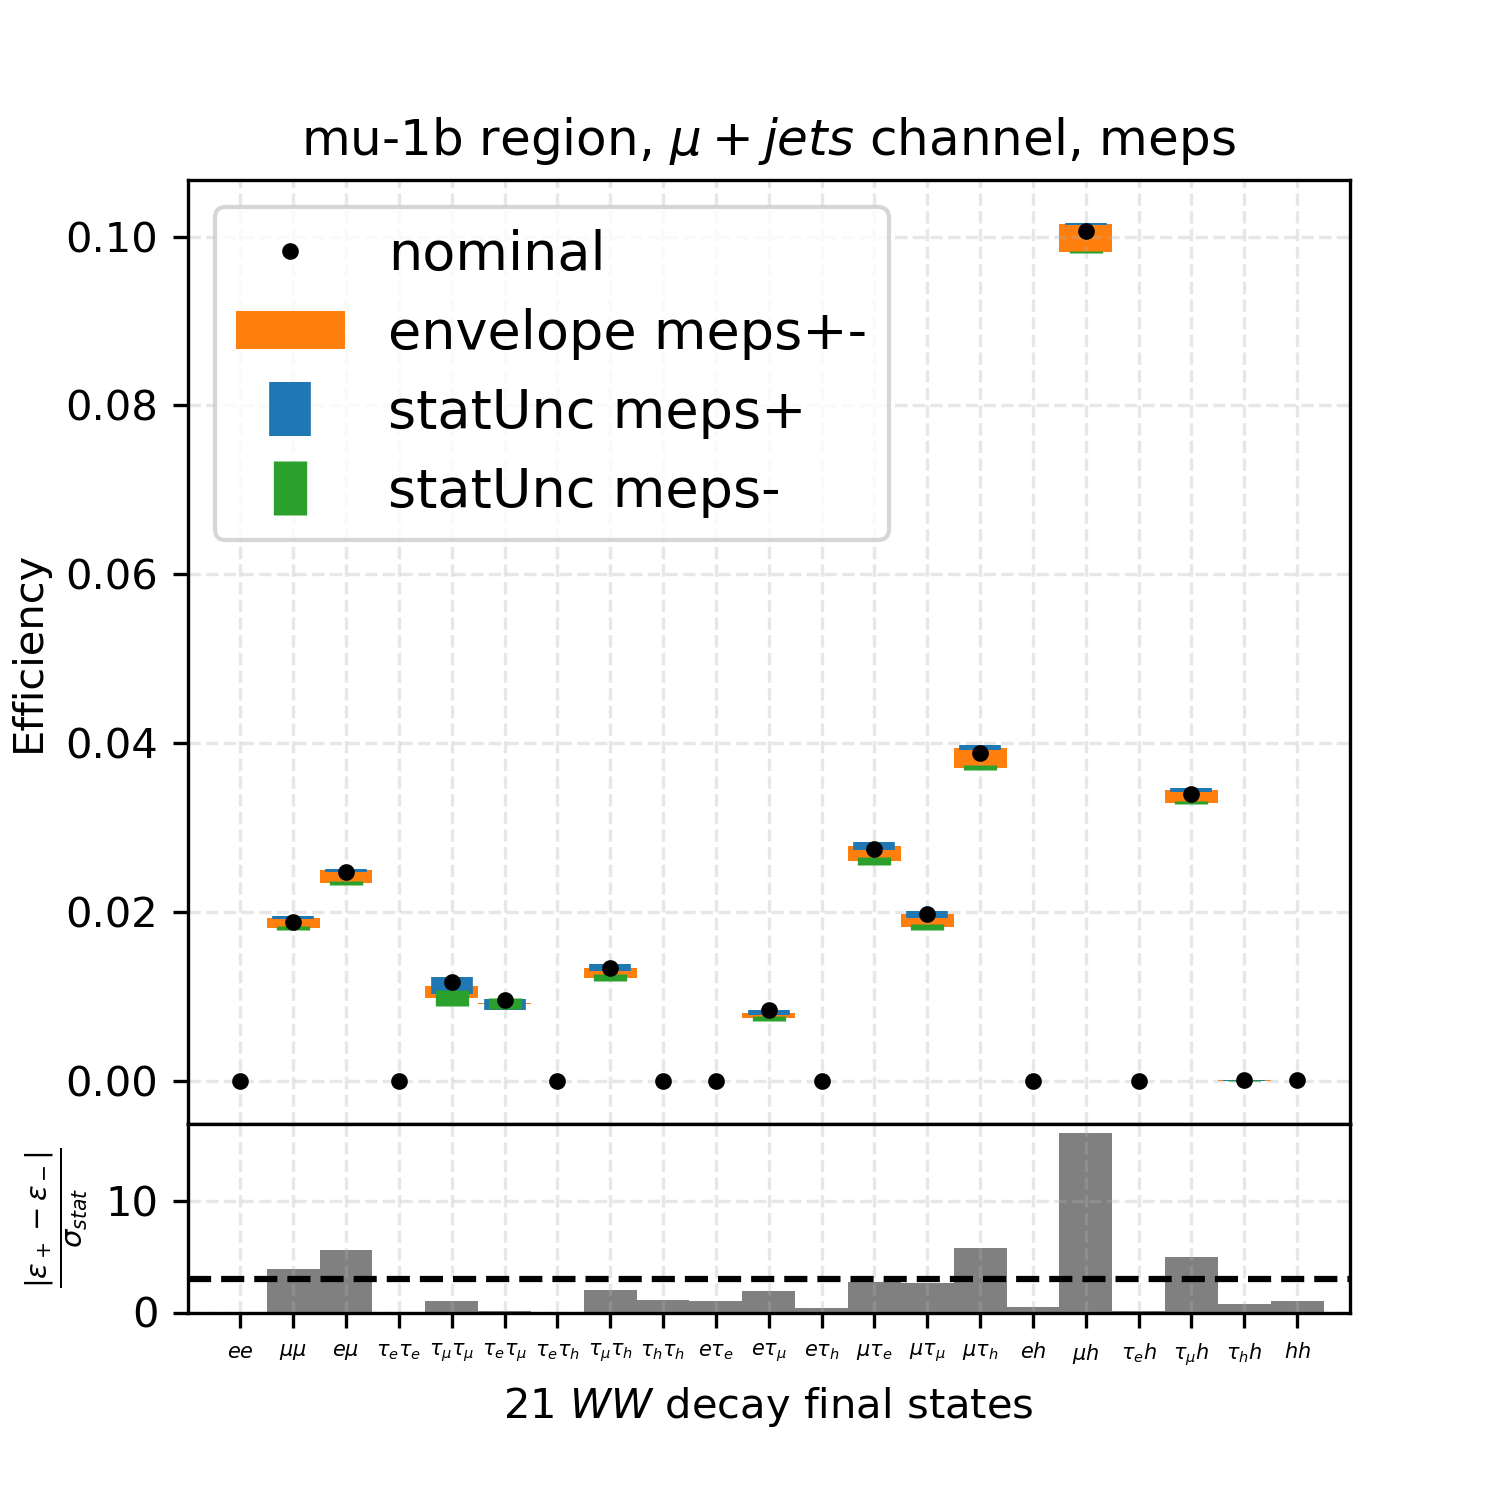
\includegraphics[width=0.24\textwidth]{chapters/Appendix/sectionTTSyst/figures/afterCorr/icata0_ch3_meps.png}

    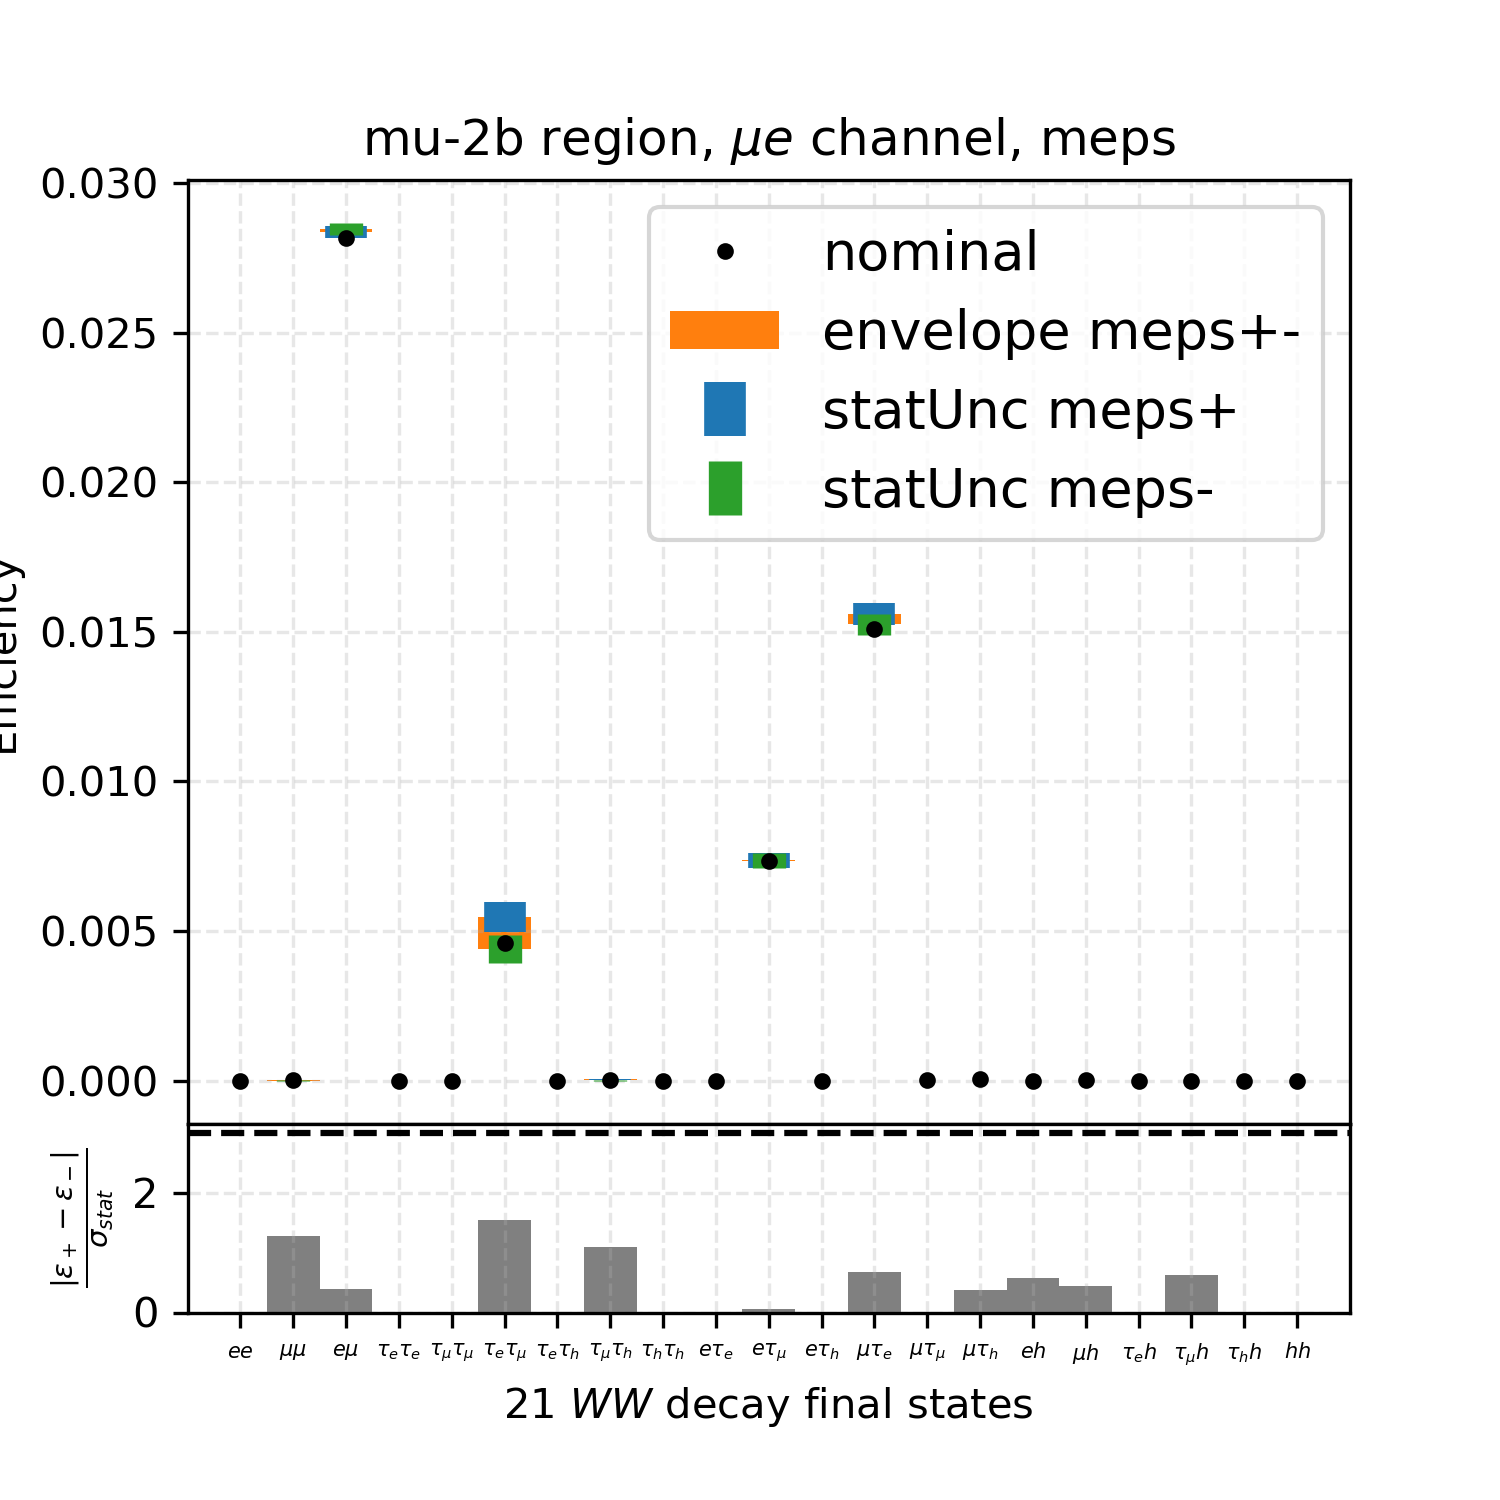
\includegraphics[width=0.24\textwidth]{chapters/Appendix/sectionTTSyst/figures/afterCorr/icata1_ch0_meps.png}
    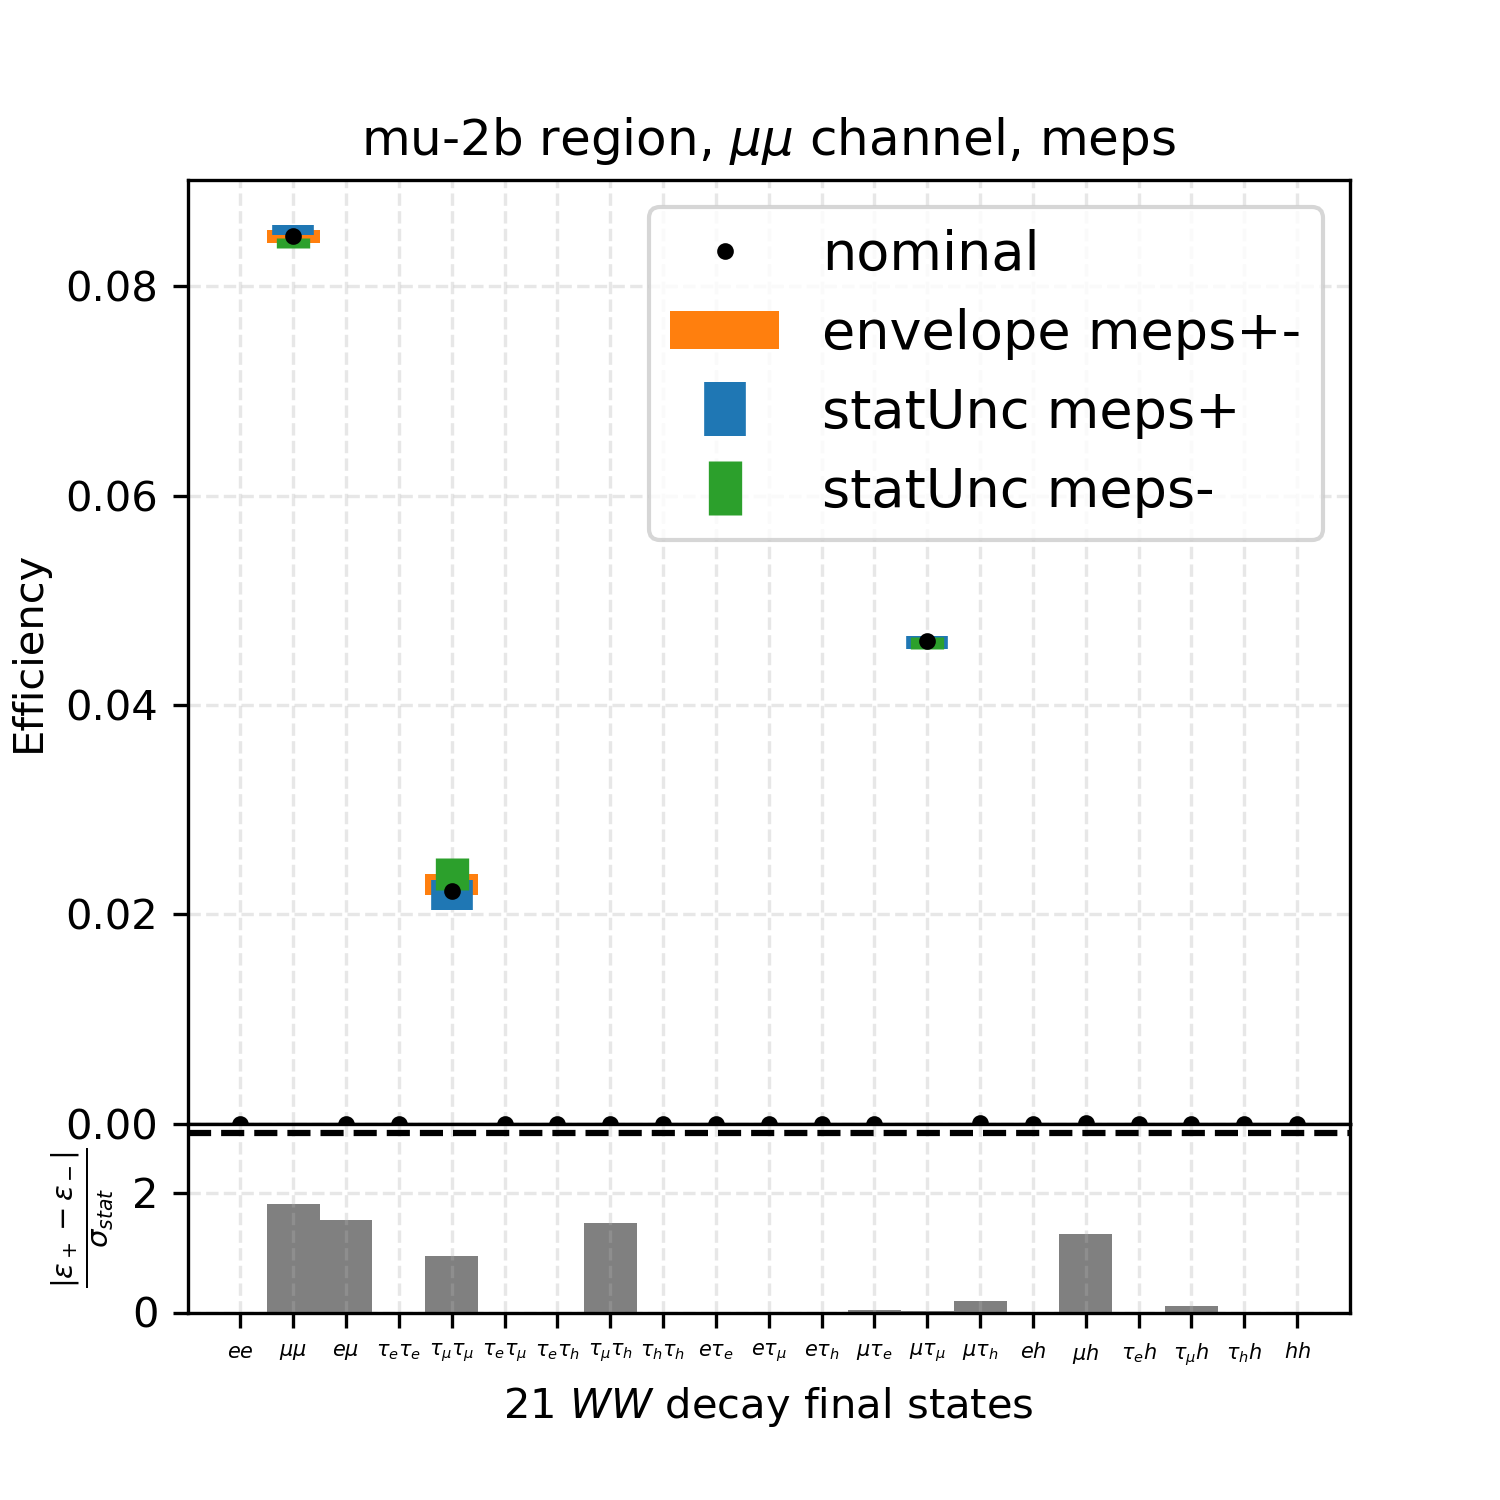
\includegraphics[width=0.24\textwidth]{chapters/Appendix/sectionTTSyst/figures/afterCorr/icata1_ch1_meps.png}
    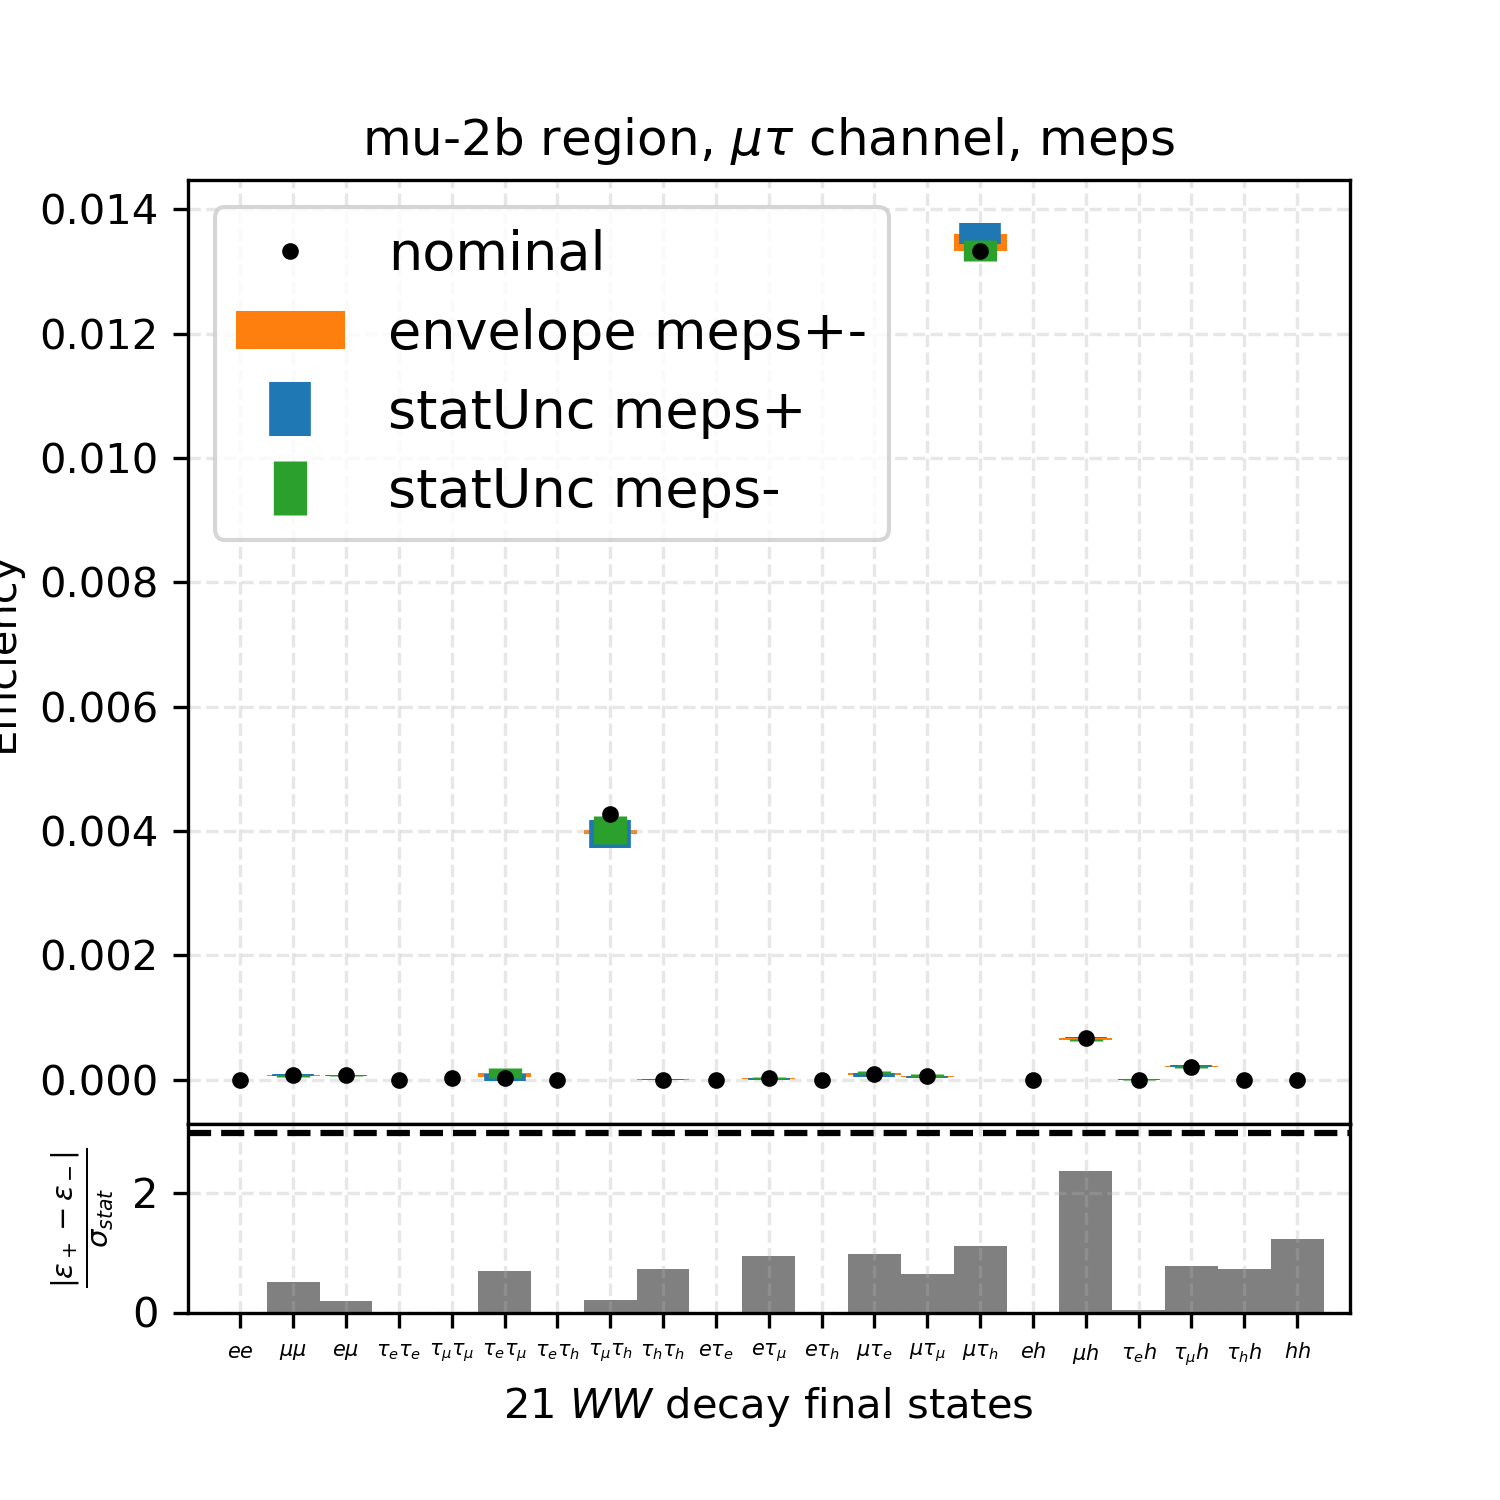
\includegraphics[width=0.24\textwidth]{chapters/Appendix/sectionTTSyst/figures/afterCorr/icata1_ch2_meps.png}
    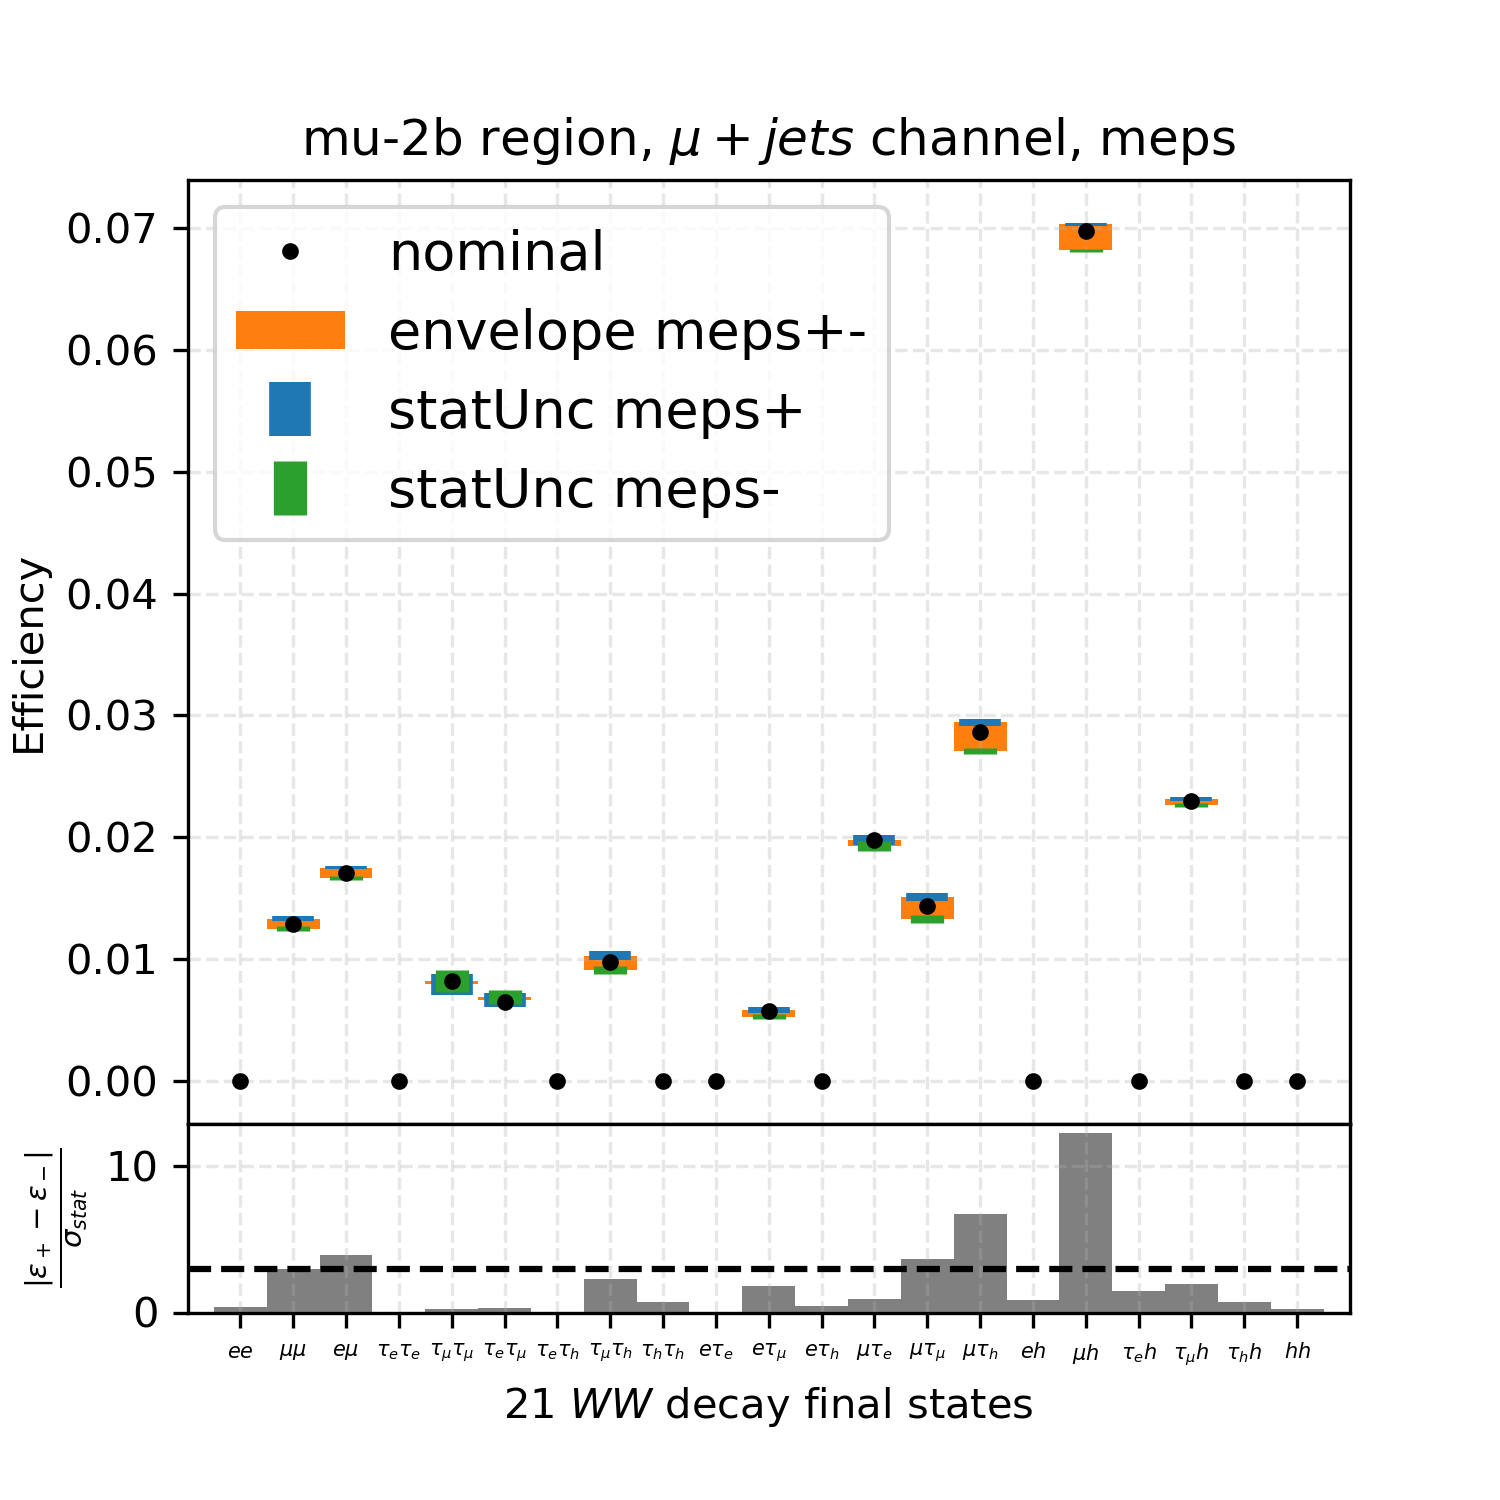
\includegraphics[width=0.24\textwidth]{chapters/Appendix/sectionTTSyst/figures/afterCorr/icata1_ch3_meps.png}
    
    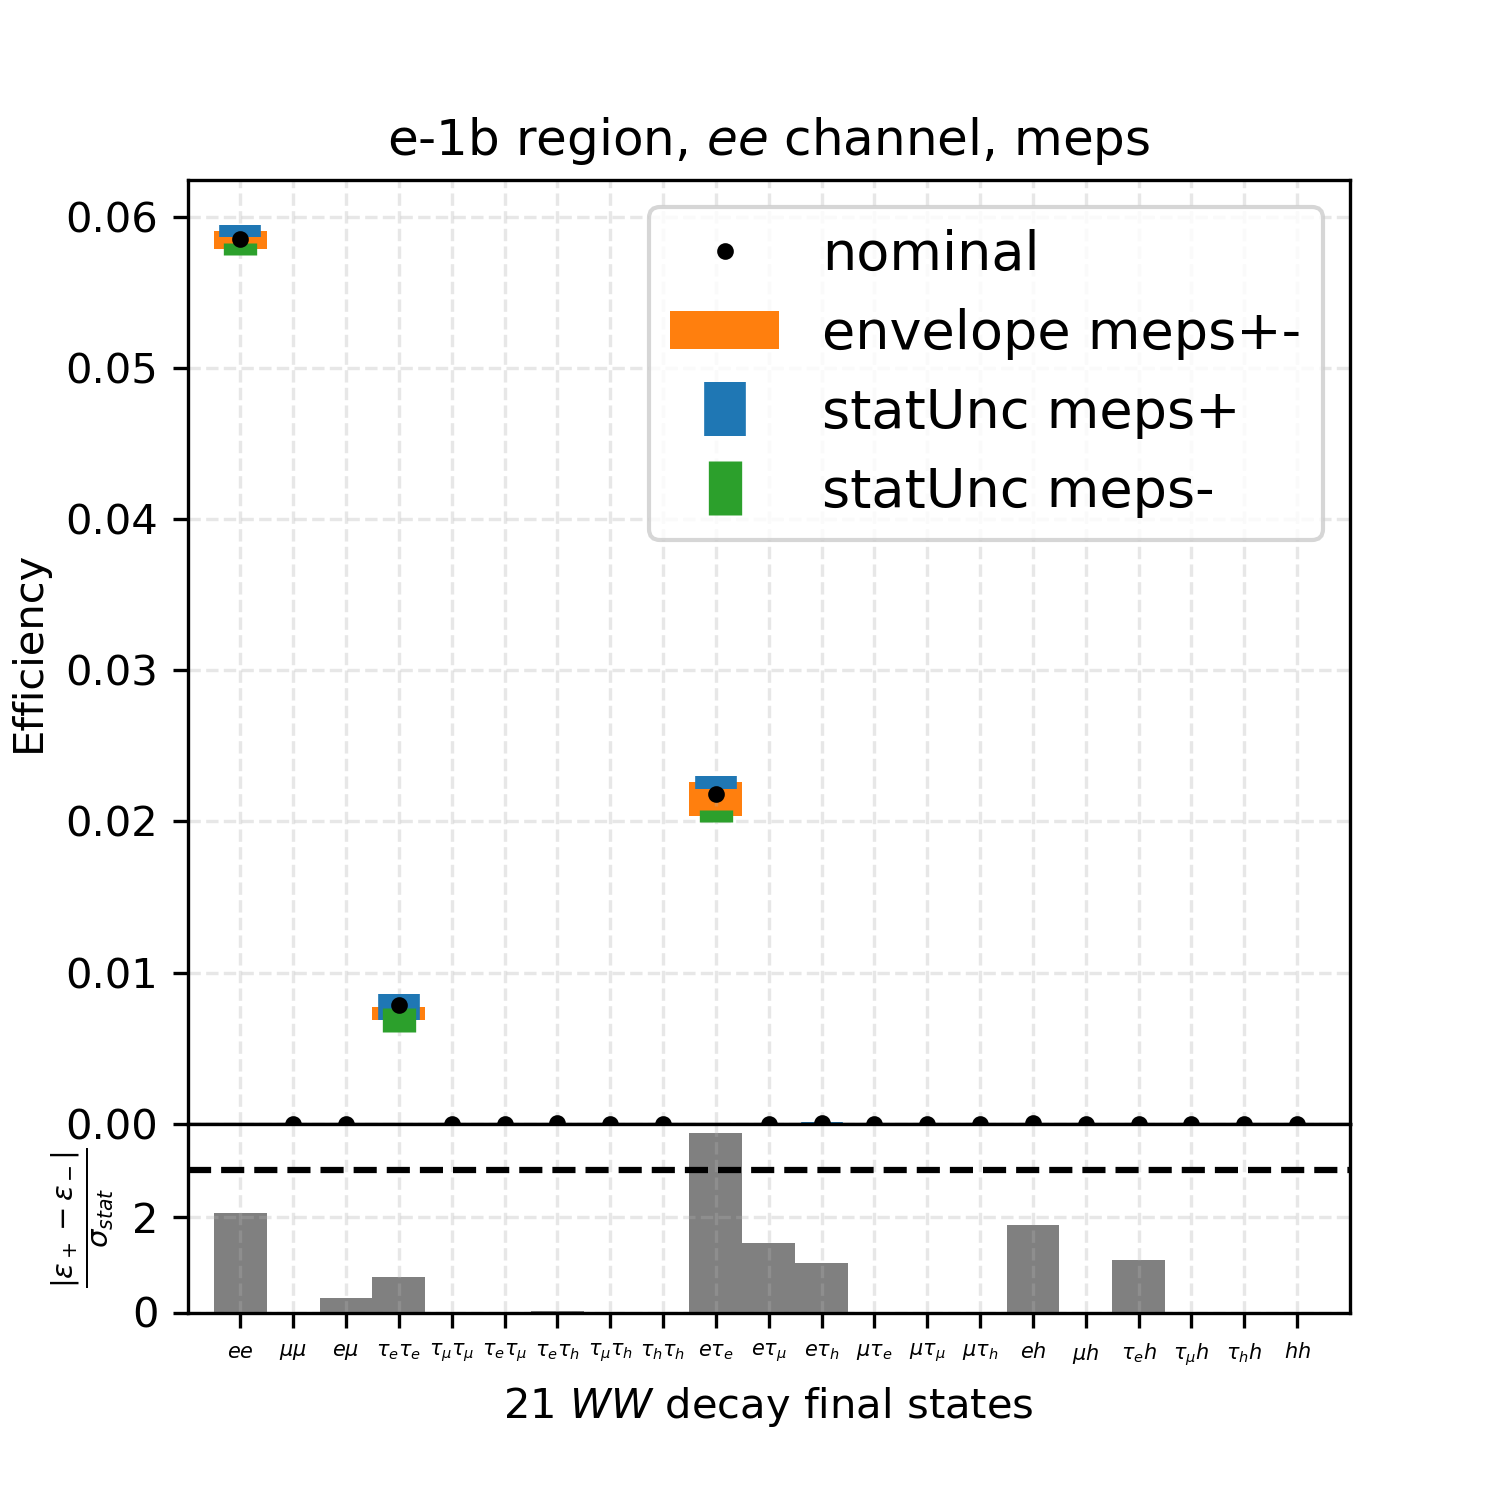
\includegraphics[width=0.24\textwidth]{chapters/Appendix/sectionTTSyst/figures/afterCorr/icata2_ch0_meps.png}
    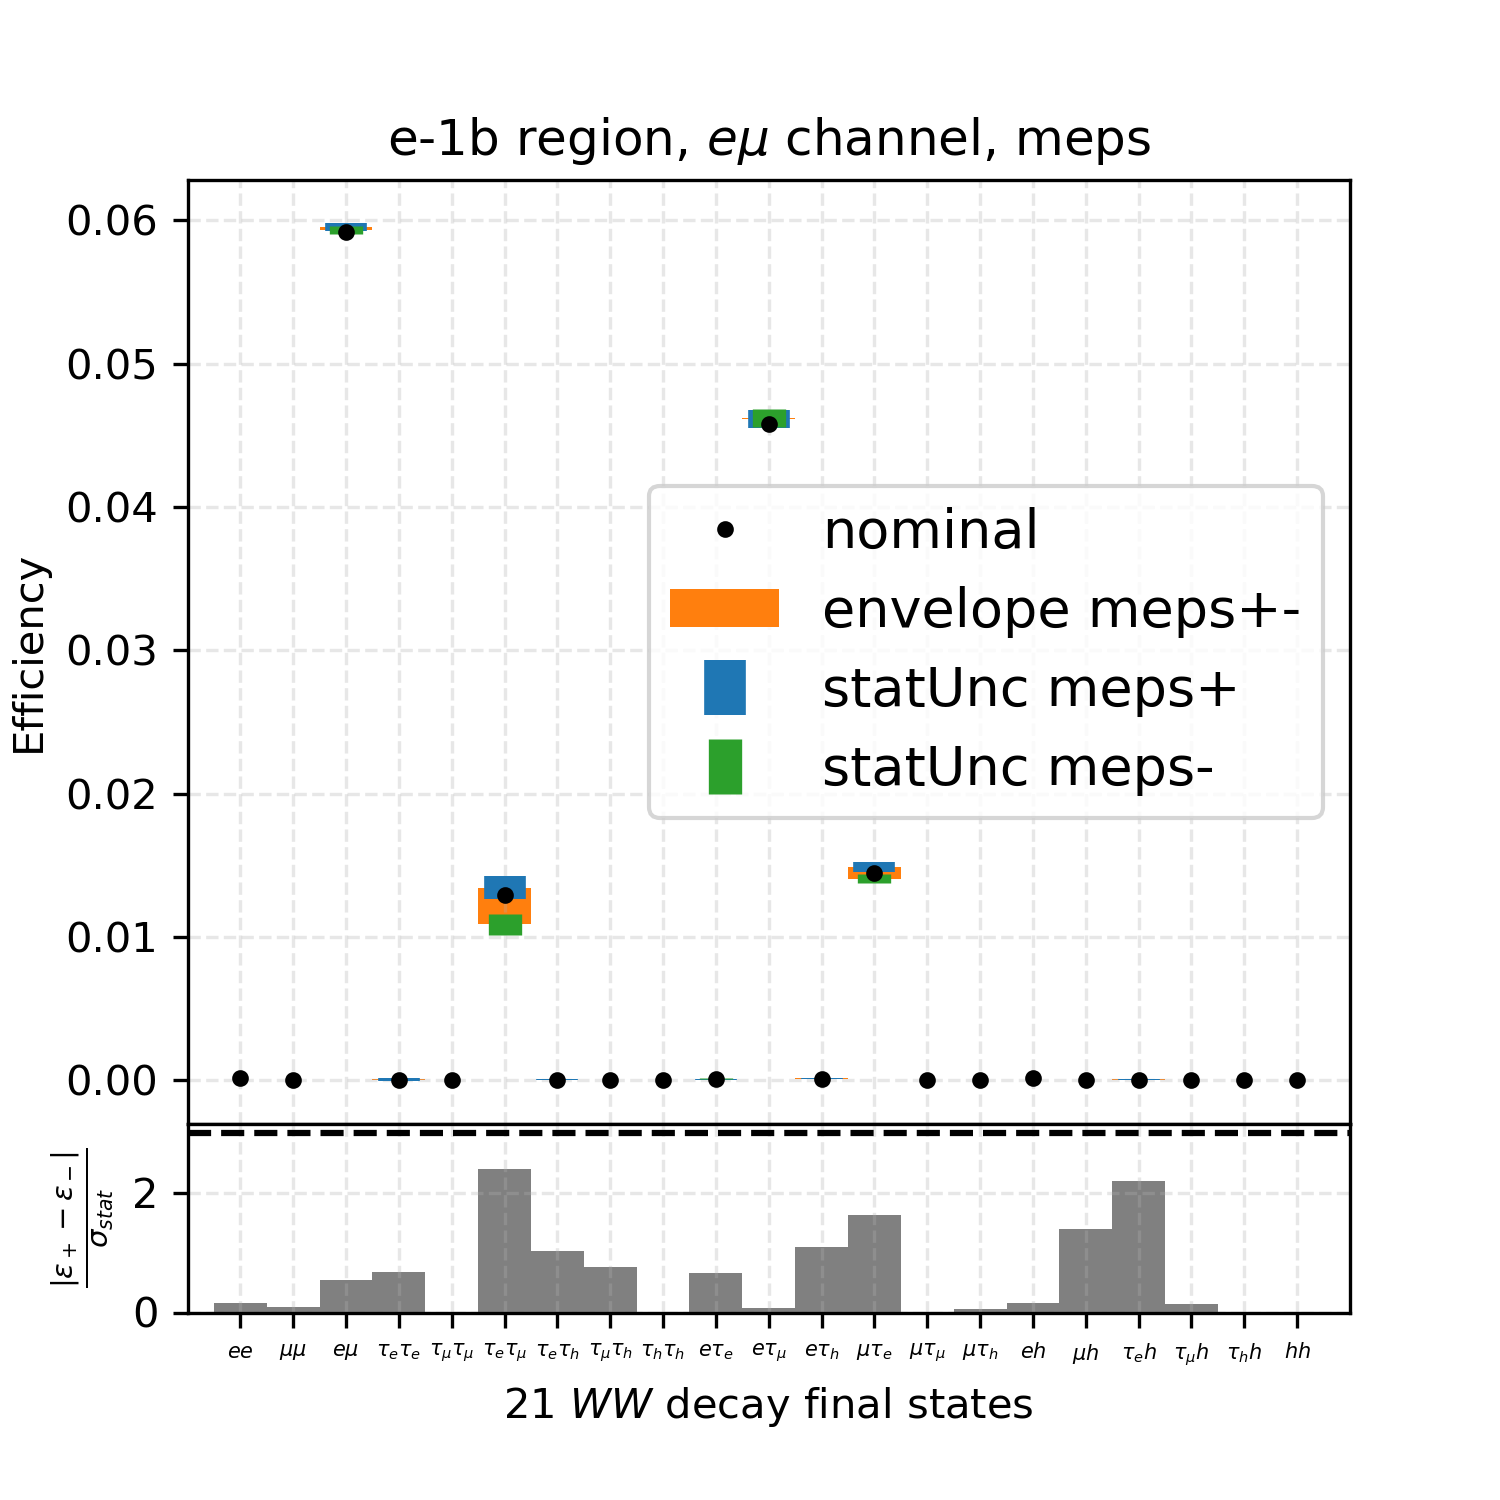
\includegraphics[width=0.24\textwidth]{chapters/Appendix/sectionTTSyst/figures/afterCorr/icata2_ch1_meps.png}
    \includegraphics[width=0.24\textwidth]{chapters/Appendix/sectionTTSyst/figures/afterCorr/icata2_ch2_meps.png}
    \includegraphics[width=0.24\textwidth]{chapters/Appendix/sectionTTSyst/figures/afterCorr/icata2_ch3_meps.png}

    \includegraphics[width=0.24\textwidth]{chapters/Appendix/sectionTTSyst/figures/afterCorr/icata3_ch0_meps.png}
    \includegraphics[width=0.24\textwidth]{chapters/Appendix/sectionTTSyst/figures/afterCorr/icata3_ch1_meps.png}
    \includegraphics[width=0.24\textwidth]{chapters/Appendix/sectionTTSyst/figures/afterCorr/icata3_ch2_meps.png}
    \includegraphics[width=0.24\textwidth]{chapters/Appendix/sectionTTSyst/figures/afterCorr/icata3_ch3_meps.png}
    
    \caption{MEPS envelops on 21 efficiencies. VTight WP is shown.}
    \label{fig:appendix:reweighttt:effAfterCorrMEPS}
\end{figure}


\begin{figure}
    \centering
    \includegraphics[width=0.24\textwidth]{chapters/Appendix/sectionTTSyst/figures/afterCorr/icata0_ch0_ue.png}
    \includegraphics[width=0.24\textwidth]{chapters/Appendix/sectionTTSyst/figures/afterCorr/icata0_ch1_ue.png}
    \includegraphics[width=0.24\textwidth]{chapters/Appendix/sectionTTSyst/figures/afterCorr/icata0_ch2_ue.png}
    \includegraphics[width=0.24\textwidth]{chapters/Appendix/sectionTTSyst/figures/afterCorr/icata0_ch3_ue.png}

    \includegraphics[width=0.24\textwidth]{chapters/Appendix/sectionTTSyst/figures/afterCorr/icata1_ch0_ue.png}
    \includegraphics[width=0.24\textwidth]{chapters/Appendix/sectionTTSyst/figures/afterCorr/icata1_ch1_ue.png}
    \includegraphics[width=0.24\textwidth]{chapters/Appendix/sectionTTSyst/figures/afterCorr/icata1_ch2_ue.png}
    \includegraphics[width=0.24\textwidth]{chapters/Appendix/sectionTTSyst/figures/afterCorr/icata1_ch3_ue.png}
    
    \includegraphics[width=0.24\textwidth]{chapters/Appendix/sectionTTSyst/figures/afterCorr/icata2_ch0_ue.png}
    \includegraphics[width=0.24\textwidth]{chapters/Appendix/sectionTTSyst/figures/afterCorr/icata2_ch1_ue.png}
    \includegraphics[width=0.24\textwidth]{chapters/Appendix/sectionTTSyst/figures/afterCorr/icata2_ch2_ue.png}
    \includegraphics[width=0.24\textwidth]{chapters/Appendix/sectionTTSyst/figures/afterCorr/icata2_ch3_ue.png}

    \includegraphics[width=0.24\textwidth]{chapters/Appendix/sectionTTSyst/figures/afterCorr/icata3_ch0_ue.png}
    \includegraphics[width=0.24\textwidth]{chapters/Appendix/sectionTTSyst/figures/afterCorr/icata3_ch1_ue.png}
    \includegraphics[width=0.24\textwidth]{chapters/Appendix/sectionTTSyst/figures/afterCorr/icata3_ch2_ue.png}
    \includegraphics[width=0.24\textwidth]{chapters/Appendix/sectionTTSyst/figures/afterCorr/icata3_ch3_ue.png}
    
    \caption{UE envelops on 21 efficiencies. VTight WP is shown.}
    \label{fig:appendix:reweighttt:effAfterCorrUE}
\end{figure}


\FloatBarrier
